\section{Foreword}\label{foreword}

\texttt{J.\ Smagorinsky}

Meteorology was one of the very first fields of physical science that
had the opportunity to exploit high speed computers for the solution of
multi-dimensional time-dependent non-linear problems. The authors of
this monograph trace the precedents from Bjerknes to von Neumann. The
numerical techniques first employed were based on a small existing body
of methodology, much of which was drawn from engineering practice, such
as the application of relaxation methods to the solution of
Poisson\textquotesingle s equation. The working repertoire of numerical
methods rapidly expanded as the physical problems grew in complexity and
as practical experience accrued. The growth was almost exclusively the
result of the innovations of the "using" physical scientists themselves.
As a consequence these advances often lacked the rigour and proof that
might have been expected from applied mathematicians. The results of
this evolution are to be found scattered throughout the meteorological
literature of the past 25 years and it became apparent that there was a
growing need for a systematic account of the rationale and development
of technique. The JOC felt that GARP\textquotesingle s needs, as
reflected by the rapid influx of new scientists into numerical
modelling, would be well served by the availability of a single
definitive source. Other related disciplines such as oceanography have
also indicated a need for a means to rapidly assimilate the accumulated
experience of meteorology. The first attempt was at the hands of two
able mathematicians, H. Kreiss and J. Oliger, who contributed a much
needed sense of mathematical unity in their monograph "Methods for the
Approximate Solution of Time-Dependent Problems" (G.P.S. No. 10, 1973).
This present volume, more specifically reflecting experience with
atmospheric models, has been written by two outstanding workers in the
field, Prof. F. Mesinger and Prof. A. Arakawa, with Dr. A. Robert as
general editor. An additional volume will be published containing
chapters on the subjects: spectral methods, global mapping problems, and
finite element methods.

\section{Introduction, general remarks about the grid point
method}\label{Chapter1}

In this chapter, following a short historical introduction on the
development and use of numerical methods in atmospheric models, methods
available for numerical solution of the differential equations governing
the atmosphere will be briefly reviewed. Then, basic elements of the
finite difference method for solving these equations will be introduced.
Finally, the concept of stability of finite difference equations, and
methods for testing the stability of such equations, will be discussed
at some length.

\subsection{\texorpdfstring{\textbf{Historical
introduction}}{Historical introduction}}\label{historical-introduction}

It is considered that Wilhelm Bjerknes (1904) was the first to point out
that the future state of the atmosphere can in principle be obtained by
an integration of differen­tial equations which govern the behaviour of
the atmo­sphere, using as initial values fields describing an observed
state of the atmosphere. Such an integration performed using numerical
methods is called numerical weather prediction. When, however, a
numerical integration is performed starting from fictitious initial
fields, it is called numerical simulation.

A first practical attempt at a numerical weather predic­tion was made by
Richardson. After very tedious and time-consuming computations, carried
out mostly during the First World War, Richardson obtained a totally
unacceptable result. Despite this, he described his method and results
in a book (Richardson, 1922), and this is today one of the most famous
in meteorology.

The wrong result obtained by Richardson, and his estimate that 64,000
men are necessary to advance the calculations as fast as the weather
itself is advancing, left some doubt as to whether the method would be
of practical use. A number of developments that followed, however,
improved the situation. Courant, Friedrichs and Lewy (1928) found that
space and time increments in integrations of this type have to meet a
certain stability criterion. Mainly due to the work of Rossby in the
late 1930\textquotesingle s, it became understood that even a rather
simple equation, that describing the conservation of absolute vorticity
following the motion of air particles, suffices for an approximate
description of large-scale motions of the atmosphere. Finally, in 1945,
the first electronic computer ENIAC (Electronic Numerical Integrator and
Computer) was constructed. The absolute vorticity conservation equation,
and this first electronic computer, were used by Charney, Fjortoft and
von Neumann in the late 1940\textquotesingle s for the first successful
numerical forecast (Charney et al., 1950).

Much faster computers, and improved understanding of computational
problems, now also enable long-term integrations of the basic primitive
equations. It is gener­ally considered that integration of the primitive
equations enables easier incorporation of various physical processes
than the integration of modified equations, that is, inte­gration of the
divergence and vorticity equations. Thus, it is mostly the primitive
equations that are used today for practical numerical forecasting by
meteorological services. Charts obtained by numerical forecasting are
used by synopticians in these services as the principal basis for
decisions on forecasts issued for public use.

A number of research groups have been actively engaged for more than a
decade in development of models for the numerical simulation of the
general circulation of the atmosphere. In such simulations starting from
a fictitious initial state, e.g. an isothermal and motionless
atmosphere, is often considered to be an advantage for the experiments.
It enables a test of the ability of the computational and physical
schemes of the model to simulate an atmosphere with statistical
properties similar to those of the real atmosphere, with no, or not
much, prior information on these properties.

Numerical models are also very frequently developed for studies of some
smaller-scale atmospheric phenomena. Foremost among these are studies of
the cumulus convec­tion problem, and simulation of processes within the
planetary boundary layer. In this text, however, we shall primarily have
in mind the application of numerical methods to prediction and
simulation of large-scale atmospheric motions.

\subsection{\texorpdfstring{\textbf{Methods for the numerical solution
of the equations of
motion}}{Methods for the numerical solution of the equations of motion}}\label{methods-for-the-numerical-solution-of-the-equations-of-motion}

Numerical solution of the equations of motion today in most cases is
performed using the \emph{grid point method}. In this method a set of
points is introduced in the region of interest and dependent variables
are initially defined and subsequently computed at these points. This
set of points is called the \emph{grid}. The words \emph{mesh or
lattice} are also used. It is necessary to have the grid points at fixed
locations in the horizontal. This means that, according to the Eulerian
system of equations, space and time coordinates are chosen as
independent variables.

A number of attempts have been made to develop atmospheric models using
an approach which is at least partly Lagrangian. Serious difficulties
are encountered when a straightforward numerical integration of the
Lagrangian system of equations is undertaken. However, it is possible to
construct methods with some Lagrangianproperties ; for example, to have
some or all of the compu­tation points moving with the fluid. In
hydrodynamics a number of such methods have proved to be very useful,
especially for some problems which are not amenable to treatment by a
strictly Eulerian technique (e.g. Harlow and Amsden, 1971). However, in
meteorology the per­formance of Lagrangian or semi-Lagrangian models
that have so far been developed has not been quite satis­factory. A
discussion of one way of constructing a Lagrangian model, and a review
of earlier attempts, can be found in a paper by Mesinger (1971).

Another possible approach is to express the spatial dependence of the
variables in terms of a series of ortho­gonal functions, and then
substitute this into the governing equations. In this way the equations
reduce to a set of ordinary differential equations, so that the
coefficients of the series can be computed as functions of time. This is
the \emph{spectral method} of solving the governing equations. Until
relatively recently it was considered that in effi­ciency the spectral
method could not be competitive with the grid point method. But the use
of the fast Fourier transform has completely changed the situation and
investigation of spectral methods is now the subject of intensive
research.

In the following we shall consider the technique of using the grid point
method, and the problems associated with it, using grid of computation
points fixed in space. This is the most direct way of solving the
equations of motion numerically. Furthermore, knowledge of this method
is necessary for the investigation and under­standing of the relative
merits of other alternatives mentioned in this section.

\subsection{\texorpdfstring{\textbf{Basic elements of the grid point
method}}{Basic elements of the grid point method}}\label{basic-elements-of-the-grid-point-method}

With the grid point method, the most common way of solving the governing
equations is to find approximate expressions for derivatives appearing
in the equations. These approximate expressions are defined using only
values of the dependent variables at the grid points, and at discrete
time intervals. Thus, they are formed using differences of dependent
variables over finite space and time intervals; for that reason this
approach is called the \emph{finite difference method}. The
approximations for derivatives are then used to construct a system of
algebraic equations that approximates the governing partial differential
equations. This algebraic system is considered valid at each of the
interior grid points of the computation region. For the initial time and
at space boundary points, additional constraints or equa­tions are
defined that approximate the initial and bound­ary conditions as
required by the physics of the problem. The set of algebraic equations
obtained in this way is then solved, usually using an electronic
computer, by a suitable step-wise procedure.

We shall now consider some basic elements of the finite difference
method. For simplicity, we start by considering a function of one
independent variable

\[u = u(x)\]

The function \emph{u} is a solution to a differential equation that we
are interested in. We want to find an approxima­tion to this solution in
a bounded region R of the inde­pendent variable, having a length
\emph{L}. The simplest way of introducing a set of grid points is to
require that they divide the region R into an integer number of
intervals of equal length \(\Delta x\). This length \(\Delta x\) is
called the \emph{grid interval}, or \emph{grid length}. Let us denote
the number of grid intervals by \emph{J}. It is convenient to locate the
origin of the \emph{x} axis at the left-hand end of the region R. Thus,
we are looking for approximations to \(u (\mathcal{x)}\) at discrete
points \(\mathcal{x = j}\Delta\mathcal{x, }\) where \emph{j} takes
integer values 0,1,2,... \emph{J}. These approximate values we shall
denote by

\[u_j = u_j(j \Delta x)\]

Thus, we are interested in finding \emph{J} + 1 values \(u_ j\)

Knowledge of a discrete set of values \(u_j\), even if the
approximations were perfect, offers, obviously, less information than
knowledge of the function \emph{u} (\emph{x}). Let us briefly consider
the situation in that respect. We shall very often find it convenient to
think of the function \emph{u} (\emph{x}) as being formed by a sum of
its Fourier compo­nents, that is

\[u( x ) = \frac{a_{0}}{2} + \sum_{n \geq 1}(\left[  a_{n}  \cos\left(2\pi n \frac{x}{L}\right) 
+ b_{n}   \sin\left(2\pi n \frac{x}{L} \right))\right]\]

Now, the available \emph{J} + 1 values \(u_j\) do not enable the
computation of all of the coefficients \(a_{n}b_{n}\); rather, they can
be used to compute only \emph{J} + 1 different coefficients. A natural
choice is to assume that the \emph{J} + 1 values \(u_j\) define the near
value \(a_{0}\) and as many as possible of the coefficients of the
Fourier components at the long wave length end of the series, that is,
coefficients for \emph{n} = 1,2,3,..., \emph{J/} 2. Of these components,
the one with the shortest wavelength will have n=J/2, with the wave
length

\[\frac{L}{n} =  \frac{2L}{j} =  \frac{2L}{\frac{L}{\Delta\mathcal{x}}} = 2\Delta\mathcal{x}\]

Having made that choice, we can say that with values \(u_{j}\) at
discrete points \(\mathcal{x =}j\Delta\mathcal{x}\) it is not possible
to resolve waves with wave length shorter than 2 \emph{∆} x.

Now let us consider the differences between values u\} that will be used
to construct approximations to deriva­tives. These differences are
called \emph{finite differences}. They can be calculated over one or
more of the intervals Ax. Depending on the relation of the points from
which the values are taken to the point where the derivative is
required, they can be \emph{centered or uncentered}. An un-centered
difference is, for example, the \emph{forward} difference

\[\Delta u_{\text{i }} = u_{j + 1}  - u_{j}\]

More often centered (or \emph{central}) differences are used, such as

\[\text{δu}_{j + \frac{1}{2}} =  u_{i + 1} -  u_{j}\]

In a centered difference the difference is between values symmetrical
about the point where the difference is being calculated.

One way to construct an approximation to a differen­tial equation is to
simply replace the derivatives by appro­priate \emph{finite difference
quotients}. For example, for the first derivative one can use the
approximation

{\[\left( \frac{d u}{d x } \right)_j \to \frac{u_{j + 1} - u_{j}}{\Delta x}\]}

The finite difference quotient here is, of course, only one of many
possible approximations to the first derivative at point j.

If a finite difference quotient, or a more complex expression, is to be
used as an approximation to a deri­vative, it is required, above all,
that this approximation be consistent. This means that the approximation
should approach the derivative when the grid interval approaches zero.
The quotient \texttt{3.1} , obviously, has that property.

Important information is obatined when the true solution
\(u (j\Delta x)\) is substituted into an approximation to the derivative
in place of the grid point values \(u_{j}\), and \(u(j\Delta x)\) is
expanded in a Taylor series about the central point. For the quotient
\texttt{3.1} this procedure gives

\[\frac{u_{j+1} - u_j}{\Delta x} \to \left( \frac{d u}{d x} \right)_j +
\frac{1}{2} \left( \frac{d^2 u}{dx^2} \right)_j \Delta x +
\frac{1}{6} \left( \frac{d^3 u}{dx^3} \right)_j
( \Delta x )^2 + \ldots\]

The difference between this expression and the derivative

\[\left( \frac{\text{du}}{\text{dx}} \right)_{j}\]

being approximated. In this case

\[\varepsilon = \frac{1}{2}\left( \frac{d^{2}u}{\text{dx}^{2}} \right)\Delta x + \frac{1}{6}\left( \frac{\text{du}^{3}}{\text{dx}^{3}} \right)_{j}\]

is called the truncation error of the approximation to the derivative.
These are terms that were "truncated off" to form the approximation. The
truncation error gives a measure of how accurately the difference
quotient approximates the derivative for small values of ∆x.

The usual measure of this is the order of accuracy of an approximation.
This is the lowest power of Ax that appears in the truncation error.
Thus, approximation (3.1) is of the first order of accuracy. We can
write

\[\varepsilon = 0(\Delta x)\]

For an approximation to the derivative to be consistent it must,
obviously, be at least first order accurate.

\subsection{\texorpdfstring{\textbf{Finite difference
schemes}}{Finite difference schemes}}\label{finite-difference-schemes}

The algebraic equation obtained when derivatives in a differential
equation are replaced by appropriate finite difference approximations is
called a finite difference approximation to that differential equation,
or a finite difference scheme. In this section we shall introduce the
concepts of consistency, truncation error, and accuracy, for a finite
difference scheme.

As an example, we shall use the linear advection equation

{\[\frac{\partial u}{\partial t} +c\frac{\partial u}{\partial x } = 0; u =u(x,t)\]}

\emph{c} is a positive constant.

It describes advection of the variable u at a constant velocity c in the
direction of the x axis. The solution to this simple equation can, of
course, also be obtained by an analytic method. It will be useful to
obtain the analytic solution first, in order to investigate properties
of numerical solutions by comparing them against known properties of the
true solution.

It is convenient to this end to change from variables \emph{x}, \emph{t}
to variables, \(\xi,\) \emph{t} with the substitution \(\xi = x - ct\).

Using the notation

\[u^{(x,t)} = U (\xi, t)\]

we obtain

\[\frac{\partial u}{\partial t} = \frac{\partial U}{\partial\xi}\frac{\partial\xi}{\partial y} +
\frac{\partial U}{\partial t}\frac{\partial t}{\partial t} =-c\frac{\partial U}{\partial\xi}+
\frac{\partial U}{\partial t}\]

\[\frac{\partial u}{\partial x} =\frac{\partial U}{\partial\xi}\frac{\partial\xi}{\partial X}
+ \frac{\partial U}{\partial t}\frac{\partial t}{\partial x}\frac{\partial U}{\partial\xi}\]

Substitution of these expressions into \texttt{g4.1} gives

\[\frac{\partial}{\partial t}U(\xi,t) = 0\]

Thus, it is seen that U cannot be a function of t, but can be an
arbitrary function of \(\xi\). A solution of \texttt{g4.1} is,
therefore,

{\[u = f(x - ct)\]}

where \emph{f} is an arbitrary function. This, we see, is the general
solution of the advection equation \texttt{g4.1}, since it can satisfy
an arbitrary initial condition

{\[u(x,0) = F(x)\]}

Thus,

{\[u = F \left( x - ct \right)\]}

is the solution of \texttt{g4.1} satisfying the initial condition
\texttt{g4.3}.

For a physical interpretation, it is often convenient to consider the
solution in the \emph{x, t} plane. In the present case, we see that the
solution takes constant values along the straight lines

\[x - ct = const.\]

These lines are the \emph{characteristics} of the advection equa­tion ;
one of them is shown in \texttt{figg:1}. We can say that the solution
propagates along the characteristics.

\begin{figure}
\centering
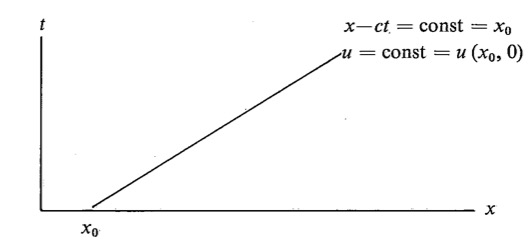
\includegraphics[width=0.8\linewidth,height=\textheight,keepaspectratio]{./pictest/pic1.jpg}
\caption{One of the characteristics of the linear advection equation
\texttt{g4.1}}
\end{figure}

Let us now construct a scheme for finding an approxi­mate solution to
\texttt{g4.1} using the grid point method.

We are now looking only for an approximate solution at the discrete
points in the \((x,t)\) plane formed by the grid shown in Fig.
\texttt{figg:1}. The approximate solution at a point
\(\left( j\Delta x, n\Delta t) \right)\) is denoted by \(u_{j}^{n}\).

\begin{figure}
\centering
\pandocbounded{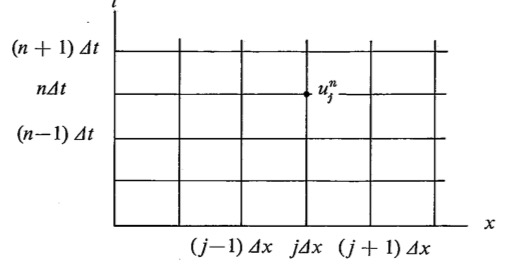
\includegraphics[keepaspectratio]{./pictest/pic2.jpg}}
\caption{}
\end{figure}

The behaviour of the true solution, which propagates along
characteristics in the (x,t) plane, suggests constructing the
approximate equation by replacing the time derivative by a forward
difference quotient, and the space derivative by a backward difference
quotient. In this way we obtain the scheme

{\[\frac{u_{j}^{n + 1} - u_{j}^{n}}{\Delta t} + c\frac{u_j^n - u_{j - 1}^n}{\Delta x} = 0\]}

This scheme could be called a forward and upstream scheme, the latter
word indicating the position of the point \(j - 1\) relative to the
advection velocity. It is, of course, only one of many possible
consistent finite difference schemes for the differential equation.
There are many schemes which approach the differential equation when the
increments \(\Delta x,\Delta t\) approach zero.

Since for small values of \(\Delta x,\Delta t\) a finite difference
equation approximates the corresponding differential equation, we can
expect that its solution will be an approximation to the solution of
that equation. We shall call solutions given by finite difference
schemes numerical solutions. There are, of course, both approximate and
numerical solutions obtained by other methods which will not be
considered in this publication. It is most convenient to study the
properties of numerical solutions when they can be compared with known
solutions of the original differential equation, which we shall refer to
as true solutions. The difference between the numerical and the true
solution

{\[u_{j}^{n}-u ( j\Delta x,n\Delta t )\]}

is the error of the numerical solution.

For obvious reasons, we cannot often expect to know the error of the
numerical solution. However, we can always find a measure of the
accuracy of the scheme by substituting the true solution
\(u \left( j\Delta x,n\Delta t \right)\) of the equation, into the
numerical scheme. Since the true solution will not satisfy the numerical
equations exactly, we will have to add an additional term to keep the
equation valid. Let us denote this term by \(\varepsilon\) . For
example, in the case of scheme \texttt{g4.5} this procedure gives

{\[\frac{u\left( j\Delta x,( n + 1 )\Delta t \right)
- u\left( j\Delta x,\Delta\text{nt} \right)}{\Delta t} 
+ c\frac{u\left( j\Delta x,n\Delta t \right) 
- u\left( \left( j - 1 \right)\Delta x,\Delta t \right)}{\Delta x} = \varepsilon\]}

The term e we shall call the truncation error of the finite difference
scheme. It shows how closely the true solution satisfies the equation of
the scheme, and, thus, gives a measure of the accuracy of the scheme.

We can obtain a more useful form for the expression for the truncation
error by performing a Taylor series expansion of the true solution about
the central space and time point. Using the original differential
equation to eliminate the leading term we obtain the truncation error
\texttt{g4.7} as

{\[\varepsilon = \frac{1}{2}\frac{\partial^{2u}}{{\partial t}^{2}}\Delta t 
+ \frac{1}{6}\frac{\partial^{3}u}{{\partial t}^{3}}\left( \Delta t \right)^{2} +\ldots-
c(\frac{1}{2}\frac{\partial^{2}u}{{\partial x}^{2}}\Delta x -
\frac{1}{6}\frac{\partial^{3}u}{{\partial t}^{3}}\left( \Delta x \right)^{2}
+\ldots )\]}

As before, these are the terms that were "truncated off" to make the
differential equation reduce to our finite difference scheme.

In the same way as for an approximation to the deri­vative, the order of
accuracy of a finite difference scheme is the lowest power of Ax and At
that appears in the truncation error. Thus, scheme \texttt{g4.5} is
first order accurate. We can write

\[\varepsilon = O \left( \Delta t \right) + O\left( \Delta x \right)\]

or

\[\varepsilon = O \left( \Delta x,\Delta t \right).\]

It is useful to make a distinction between orders of accuracy in space
and in time, especially when the lowest powers of \(\Delta x\) and
\(\Delta t\) are not the same. As before, a necessary condition for
consistency of a scheme is that it be at least of the first order of
accuracy.

\subsection{\texorpdfstring{\textbf{Convergence}}{Convergence}}\label{Section1.5}

The truncation error of a consistent scheme can be made arbitrarily
small by a sufficient reduction of the increments \(\Delta x\) and
\(\Delta t\). Unfortunately, we cannot be sure that this will also
result in a reduction of the error of the numerical solution. For that
reason, we return to consideration of the error

\[u_j^n-u\left( j\Delta x,n\Delta t \right).\]

Following Richtmyer and Morton (1967) we ask two questions:

(a) What is the behavior of the error
\(u_{j}^{n} - u\left( j\Delta x,n\Delta t \right)\) when, for a fixed
total time \(n \Delta t\) the increments \(\Delta x , \Delta t\)
approach zero ?

(b) What is the behavior of the error
\(u_{j}^{n} - u\left( j\Delta x,n\Delta t \right)\) when, for fixed
values of \(\Delta x, \Delta t\), the number of time steps \emph{n}
increases?

The answer to the first of these questions depends on the convergence of
the numerical solution : if the error approaches zero as the grid is
refined ( as \(\Delta x, \Delta t \rightarrow 0\) ) the solution is
called convergent. If a scheme gives a convergent solution for any
initial conditions, then the scheme also is called convergent.

Consistency of a scheme does not guarantee conver­gence. We shall
illustrate this by a simple example. We still consider the scheme
\texttt{g4.5}; its truncation error \texttt{g4.8} approaches zero as the
grid is refined, and, there­fore, this is a consistent scheme. But
consider the numerical solution, when the grid lines and
character­istics are as shown in \texttt{figg:3}. The characteristic
passing through the grid point taken as the origin in this example
passes through another grid point, A, denoted by a square. Thus, the
true solution at A, is equal to the initial value at the origin. However
the numerical solution given by \texttt{g4.5} A is computed using the
values at points denoted by circles. The shaded domain, including all of
these points, is called the domain of dependence of the numerical
scheme. The grid point at the origin is outside that domain, and, thus,
cannot affect the numerical solution at \(A_0\). Therefore, the error
can be arbitrarily great. If the space and time steps were reduced by
the same relative amount, say to one half of their values in the figure,
the domain of dependence would still remain the same, and this situation
would not change. Thus, as long as the ratio of the steps \(\Delta x\)
and \(\Delta t\) remains the same, refinement of the grid cannot bring
about a reduction in the error of the numerical solution.

\[x - ct = const\]

\begin{figure}
\centering
\pandocbounded{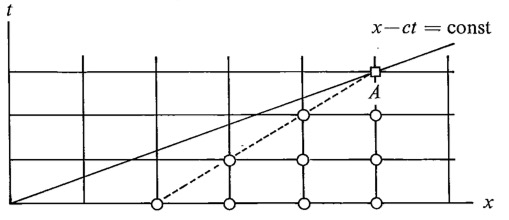
\includegraphics[keepaspectratio]{./pictest/pic3.jpg}}
\caption{}
\end{figure}

A necessary condition for convergence of a scheme is, obviously, that
the characteristic defining the true solu­tion at a grid point is inside
the domain of dependence of the numerical solution at that point. In our
example, this will happen when the slope of the characteristics is
greater than the slope of the dashed line bounding the domain of
dependence, that is, when

{\[c\Delta t \leq \Delta x\]}

Thus, this is a necessary condition for convergence of \texttt{g4.5}.

\subsection{\texorpdfstring{\textbf{Stability}}{Stability}}\label{stability}

The answer to the second question raised at the begin­ning of the
Section \texttt{Section1.5} depends on the stability of the numer­ical
solution. A rigorous definition of stability employs the concepts of
functional analysis, and refers to the boundedness of the numerical
solution only (e.g. Richt-myer and Morton, 1967). The difficulties in
defining stability are caused by the fact that the true solution, in
general, does not have to be bounded. However, when we know that the
true solution is bounded, as in the equations we are interested in here,
we can use a definition referring to the boundedness of the error
\(u_{j}^{n} - u\left( j\Delta x,n\Delta t \right)\text{. }\) We sat that
a solution \(u_{j}^{n}\) is stable if this error remains bounded as n
increases, for fixed values of \(\Delta x,\Delta t.\) As before, we say
that a finite difference scheme is stable if it gives a stable solution
for any initial conditions.

Stability of a scheme is a property of great practical significance.
There are consistent schemes, of a high order of accuracy, that still
give solutions diverging unacceptably fast from the true solution. Thus,
conditions for stability, if any, should be known. There are three
methods that can be used to investigate the stability of a scheme, and
we shall give an example of each of these methods. We shall do this by
considering again the forward and upstream scheme \texttt{g4.5}).

\emph{Direct method}. Since we know that the true solution is bounded,
it suffices to test the boundedness of the numer­ical solution. The
scheme \texttt{g4.5} can be written as

{\[u_{j}^{n + 1} = \left( 1 - \mu \right)u_{j}^{n}+ \mu u_{j - 1}^{n}\]}

where

\[\mu \equiv C\Delta t/\Delta x.\]

If \(1 - \mu \geq 0,\) which happens to be also the necessary condition
for convergence, we will have

{\[\left| u_{j}^{n + 1} \right| \leq \left( 1 - \mu \right)\left| u_{j}^{n} \right| + \mu\left| u_{j - 1}^{n} \right|.\]}

We can apply this at the point where at time level \emph{n + 1} ,
\(\left| u_{j}^{n + 1} \right|\) is a maximum,
\({Max}_{(j)} \left | u_{j}^{n + 1} \right|\). The right side of
\texttt{g6.2} can only be increased by replacing
\(\left| u_{j}^{n} \right|\) and \(\left| u_{j-1}^{n} \right|\) by the
maximum value at level n, \({Max}_{(j)} \left| u_{j}^{n} \right|\).The
two terms on the right side can then be added, and we obtain

\[{Max}_{(j)} \left| u_{j}^{n + 1} \right| \leq {Max}_{(j)}\left| u_{j}^{n} \right|\]

This proves the boundedness of the numerical solution. Hence,
\(1 - \mu \geq 0\) is seen to be a sufficient condition for stability of
\texttt{g6.1}.

This direct testing of the stability is simple. Unfortun­ately, as might
be anticipated from the argument, it is successful only for a rather
limited number of schemes.

\emph{Energy method}. This method is of a much wider appli­cability, and
can be used even for nonlinear equations. If we know that the true
solution is bounded, we test whether

\[{\sum_{j}^{}\left( u_{j}^{n} \right)}^{2}\]

is also bounded.

If it is, then every value \(u_{j}^{n}\) must be bounded, and the
stability of the scheme has been proved. The method is called the energy
method since in physical applications \(u^{2}\) is often propor­tional
to some form of energy.

Of course, there are examples when this is not so.

Squaring \texttt{g6.1} and summing over \emph{j} we obtain

{\[{\sum_{j}^{}\left( u_{j}^{n + 1} \right)}^{2} =
\sum_{j}^{}\left\lbrack \left( 1 - \mu \right)^{2}\left( u_{j}^{n} \right)^{2} + 
2\mu\left( 1 - \mu \right)u_{j}^{n}u_{j - 1}^{n} + \mu^{2}\left( u_{j - 1}^{n} \right)^{2} \right\rbrack\]}

We shall assume a cyclic boundary condition, for example
\(u_{- 1} \equiv u_{j}\), then

{\[{\sum_{j}^{}\left( u_{j - 1}^{n} \right)}^{2} =  {\sum_{j}^{}\left( u_{j}^{n} \right)}^{2}\]}

Now, using Schwarz’s inequality

\[\sum_{}^{}{ab \leq \sqrt{\sum_{}^{}a^{2}}}\sqrt{\sum_{}^{}b^{2}}\]

and \texttt{g6.4}, we can write

{\[\sum_{j}^{}u_{j}^{n}u_{j - 1}^{n} \leq \sqrt{\sum_{j}^{}\left( u_{j}^{n} \right)^{2}}\sqrt{\sum_{j}^{}
\left( u_{j - 1}^{n} \right)^{2}} =\sum_{j}^{}\left( u_{j}^{n} \right)^{2}\]}

Using \texttt{g6.4} and \texttt{g6.5} we see that, if
\(1 - \mu \geq 0\), \texttt{g6.3} gives the inequality

\[{\sum_{j}^{}\left( u_{j}^{n + 1} \right)}^{2} \leq \left\lbrack \left( 1 + \mu \right)^{2} +
2\mu\left( 1 - \mu \right) + \mu^{2} \right\rbrack\sum_{j}^{}\left( u_{j}^{n} \right)^{2}\]

or

\[{\sum_{j}^{}\left( u_{j}^{n + 1} \right)}^{2} \leq \sum_{}^{}\left( u_{j}^{n} \right)^{2}\]

Thus, \( 1 - \mu \leq 0\), coupled with the cyclic boundary condi­tion,
is proved to be a sufficient condition for stability of \texttt{g6.1}.

\emph{Von Neumann\textquotesingle s method}. Von
Neumann\textquotesingle s, or the Fourier series method is the most
frequently used method.

We will usually not be able to use it to test the stability of nonlinear
equations, and will have to resort to the analysis of their linearized
versions. A solution to a linear equation, however, can be expressed in
form of a Fourier series, where each harmonic component is also a
solution. Thus, we can test the stability of a single harmonic solution
; stability of all admissible harmonics will then be a necessary
condition for stability of the scheme.

For an illustration of this method, it is useful first to obtain an
analytic solution of the equation \texttt{g4.1}

\[\frac{\partial u}{\partial t}+c \frac{\partial u}{\partial x}=0\]

in the form of a single harmonic

{\[u\left( x,t \right) = Re\left\lfloor U\left( t \right)e^{\text{ikx}} \right\rfloor\]}

Here \emph{U(t)} is the wave amplitude, and k the wave number.
Substituting this into the preceding equation we obtain

\[\frac{\text{dU}}{d t} +ikU = 0\]

Thus, the problem of solving a partial differential equation has been
reduced to that of solving this ordinary differen­tial equation. Its
solution is

\[U(t) =U(0)e^{- ikct}\]

where U(0) is the initial value of the amplitude. Hence, the desired
harmonic solution is

{\[u\left( x,t \right) =Re \left\lbrack U\left( 0 \right)e^{\text{ik}\left( x - ct \right)} \right\rbrack\]}

Each wave component is, thus, advected at a constant velocity c along
the x axis with no change in amplitude.

Returning to the von Neumann method, we now look for an analogous
solution of the finite difference equation \texttt{g6.1}. Into this
equation we substitute a solution of the form

{\[u_{j}^{n} = Re \left\lbrack U^{\left( u \right)}e^{ikj\Delta x} \right\rbrack\]}

Here \(U^{\text{n }}\) is the amplitude at time level n. This
substitu­tion shows that \texttt{g6.8} is a solution provided that

{\[U^{n + 1} = \left( 1 - \mu \right)U^{\left( n \right)}  + \mu U^{\left( n \right)}e^{- ik\Delta x}\]}

An equation of this kind enables analysis of the behavior of the
amplitude \(U^{\text{n }}\) as n increases.

To this end we define an \emph{amplification factor}
\(\left| \lambda \right|\) by

{\[U^{n + 1} \equiv \lambda U^{n}\]}

This gives

\[|U^{n + 1}| = |\lambda | | U^{(n)} |.\]

For each harmonic solution \texttt{g6.8} to be stable it is required
that

\[|U^{n}| =|\lambda |^n | U^{(0)} | \leq B\]

where B is a finite number. This gives

\[n\log |\lambda | \leq \log \frac{B}{U^0} \equiv B'\]

where \emph{B\textquotesingle{}} is a new constant. Since
\(n = \frac{t}{\Delta t}\), the necessary condition for stability
becomes

{\[\log |\lambda | \leq \frac{B'}{t} \Delta t\]}

Now, suppose that we require boundedness of the solution for a finite
time \emph{t}. Condition \texttt{g6.11} can then be written as

\[\log|\lambda| \leq 0( \Delta t )\]

If we now define

\[\left| \lambda \right| \equiv 1 + \delta\]

we see, in view of the power series expansion of
\(\log\left( 1 + \delta \right)\), that the stability condition obtained
is equivalent to

\[\delta \leq 0\left( \Delta t \right)\]

or

{\[|\lambda| \leq 1 + O (\Delta t)\]}

This is the \emph{von Neumann necessary condition for stability}.

The von Neumann condition allows an exponential, but no faster, growth
of the solution. This, of course, is needed to analyze cases when the
true solution grows exponentially. However, when we know that the true
solution does not grow, as in our example \texttt{g6.7}, it is customary
to replace \texttt{g6.12} by a sufficient condition

{\[|\lambda| \leq 1\]}

This condition is much less generous than that required by the original
definition of stability. Returning to our example, substitution of
\texttt{g6.10} into \texttt{g6.9} gives

{\[\lambda = 1 - \mu + \mu e^{-ik\Delta x}\]}

From this we obtain

{\[\lambda^{2} =1 - 2\mu\left( 1 - \mu \right)\left( 1 - \cos{k\Delta x} \right)\]}

and, therefore, \(1 - \mu \geq 0 \) is again found to be a sufficient
condition for stability of \texttt{g6.1}.

An equation such as \texttt{g6.15} gives further information about the
behavior of the numerical solution. This can be obtained by studying the
variation of \(|\lambda|\) with \(\mu\) for various fixed values of
\(k\Delta x\). To this end we plot the \(|\lambda|^{2}\) curves ;
\texttt{g6.15} shows that in the present case all of these curves are
parabolas. Furthermore, recall that the minimum resolvable wave length
is \(2 \Delta x\). Thus, the maximum value that wave number k can take
is \(\frac{\pi}{\Delta x}\). We thus plot the \(|\lambda|^{2}\) curves
for this maximum value \(k = \frac{\pi}{\Delta\text{x}}\) (or wave
length \(L = 2\Delta x\), and for half this value,
\(k = \frac{\pi}{2\Delta x\left( L - 4\Delta x \right)}\), and a quarter
of this value,
\(k = \frac{\pi}{4\Delta x\left( L - 8\Delta x \right)}\).

The first derivative

\[\frac{d|\lambda|^2}{d\mu} = - 2( 1 - 2\mu)( 1 - \cos{k \Delta x} )\]

shows that all the \(|\lambda|^{2}\) curves have minima at
\(\mu = \frac{1}{2}\). This information, in addition to calculation of
the ordi­nales of \texttt{g6.15} at \(\mu = \frac{0.1}{2}\) and 1,
suffices for sketching

\begin{figure}
\centering
\pandocbounded{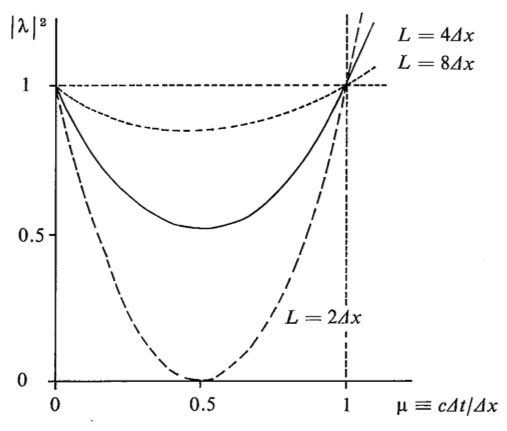
\includegraphics[keepaspectratio]{./pictest/pic4.jpg}}
\caption{}
\end{figure}

the graphs of the \(\left| \lambda \right|^{2}\) curves as shown in
\texttt{figg:1}. In general, as the wave length L increases, that is, as
k approaches zero, the amplification factor approaches unity for any
value of the parameter \(\mu\).

The figure shows that within the stable region the scheme is damping for
all values \(\mu \leq 1\). The damping increases as the wave length
decreases. Since the true solution has a constant amplitude, this
damping reveals an error due to finite differencing. We see that this
error increases as the wave length decreases. At the shortest resolvable
wave length, \(L = 2\Delta x\), the error may be very great unless At is
extremely small. It is even possible for this wave to be completely
removed after only a single time step ! The dependence of the error on
wave length, as seen here, might have been anticipated by considering
representation of harmonics of various wave lengths by the finite
difference grid. The shortest resolvable wave, with only two data points
per wave length, is very poorly represented ; as the wave length
increases, the representa­tion by a finite difference grid improves, and
approaches the continuous representation as the wave length tends to
infinity.

There exists a wealth of more precise definitions of stability and
convergence, as well as stability criteria. For a further discussion of
these subjects, and of the relation between the properties of stability
and conver­gence, the interested reader is referred to the book by
Richtmyer and Morton (1967) and to the publication by Kreiss and Oliger
(1973). However, for application of numerical methods to atmospheric
models, it is more important to discuss other problems than to refine
the stability and convergence concepts beyond the outline given here.
These numerical problems, such as phase speed errors and computational
dispersion, nonlinear instability, effect of the space-time grid on the
properties of the numerical solution, and, also the ideas behind and
properties of the great variety of schemes that are currently being used
in atmospheric models, will be discussed in the remaining chapters of
this publication.

\section{Time Differencing Schemes}\label{Chapter2}

In this chapter we consider ordinary differential equa­tions with one
dependent and one independent variable. Although atmospheric models are
essentially always models for solving a complex set of partial
differential equations, in some formulations the numerical solution of
ordinary differential equations forms an important part of the
computational procedure. For instance in spectral models the governing
partial differential equa­tions reduce to a set of ordinary differential
equations for the expansion coefficients as dependent variables. A set
of ordinary differential equations will also be obtained if a Lagrangian
method is used, in which the computa­tional points move with the fluid.
But, most of all, schemes for solving ordinary differential equations
are of interest here since they are often used without modi­fication to
construct approximations to the time deri­vative terms in the governing
partial differential equa­tions. Knowledge of the properties of schemes
for solving ordinary differential equations will then be used in
inves­tigating the properties of more complex schemes for solving the
partial differential equations.

With that in mind, we shall here first define some of the schemes that
will be interesting to analyze. Then we shall investigate the behaviour
of numerical solutions obtained when these schemes are used for two
specific ordinary differential equations: the oscillation (or frequency)
equation, and the friction equation. These equations will serve as
prototypes for later extension of the results to advection,
gravity-inertia wave, and diffusion processes within the atmospheric
primitive equations.

\subsection{\texorpdfstring{\textbf{Definitions of some
schemes}}{Definitions of some schemes}}\label{Section2.1}

Schemes used for the time derivative terms within the primitive
equations are relatively simple, usually of the second and sometimes
even only of the first order of accuracy. There are several reasons for
this. First, it is a\textquotesingle{} general experience that schemes
constructed so as to have a high order of accuracy are mostly not very
successful when solving partial differential equa­tions. This is in
contrast to the experience with ordinary differential equations, where
very accurate schemes, such as the Runge-Kutta method, are extremely
reward­ing. There is a basic reason for this difference. With an
ordinary differential equation, the equation and a single initial
condition is all that is required for an exact solution. Thus, the error
of the numerical solution is entirely due to the inadequacy of the
scheme. With a partial differential equation, the error of the numerical
solution is brought about both by the inadequacy of the scheme and by
insufficient information about the initial conditions, since they are
known only at discrete space points. Thus, an increase in the accuracy
of the scheme improves only one of these two components, and the results
are not too impressive.

Another reason for not requiring a scheme of high accuracy for
approximations to the time derivative terms is that, in order to meet a
stability requirement of the type discussed in the preceding chapter, it
is usually necessary to choose a time step significantly smaller than
that required for adequate accuracy. With the time step usually chosen,
other errors, for example in the space differencing, are much greater
than those due to the time differencing. Thus, computational effort is
better spent in reducing these other errors, and not in increasing the
accuracy of the time differencing. This, of course, does not mean that
it is not necessary to consider carefully the properties of various
possible time differencing schemes. Accuracy, is only one important
consideration in choosing a scheme.

To define some schemes, we consider the equation

{\[\frac{\text{dU}}{\text{dt}} = f( U,t) \quad  U = U(t)\]}

The independent variable t is here called time. We divide the time axis
into segments of equal length \(\Delta t\). We shall denote by
\(U^{\left( n \right)}\) the approximate value of U at time
\(n\Delta t\). We assume that we know at least the first of the values
\(U^{\left( n \right)}\), \(U^{\left( n - 1 \right)}\) ... and we want
to construct a scheme for computation of an approximate value
\(U^{\left( n + 1 \right)}\). These are many possibilities.

\subsubsection{\texorpdfstring{\emph{Two level
schemes}}{Two level schemes}}\label{two-level-schemes}

These are schemes that relate values of the dependent variable at two
time levels : n and n + 1. Only a two level scheme can be used to
advance an integration over the first time step, when just a single
initial condition is available. With such a scheme we want to
approximate the exact formula

{\[U^{( n + 1 )} = U^{\left( n \right)} + \int_{n\Delta t}^{(n+1)\Delta t}f\left( U,t \right)\text{dt}\]}

We shall first list several schemes which do not use an iterative
procedure.

\paragraph{\texorpdfstring{\emph{Euler (or forward)
scheme}}{Euler (or forward) scheme}}\label{euler-or-forward-scheme}

This is the scheme

{\[U^{\left( n + 1 \right)} = U^{\left( n \right)} + \Delta t \bullet f^{\left( n \right)}\]}

where

\[f^{\left( n \right)} \equiv f\left( U^{\left( n \right)},n\Delta t \right)\]

The truncation error of this scheme is \(O\left( \Delta t \right)\).
Thus, this is a first order accurate scheme. For the integrand in
\texttt{h1.2} we have here taken a constant value equal to that at the
lower boundary of the time interval. Thus, \(f\) in \texttt{h1.3} is not
centered in time, and the scheme is said to be uncentered. In general,
uncentered schemes will be found to be of the first order of accuracy,
and simple centered schemes to be of the second order of accuracy.

\paragraph{\texorpdfstring{\emph{Backward
scheme}}{Backward scheme}}\label{backward-scheme}

We can also take a constant value of \(f\) equal to that at the upper
boundary of the time interval. We then obtain

{\[U^{( n + 1 )} = U^{( n )} + \Delta t  f^{\left( n + 1 \right)}\]}

If, as here, a value of \(f\) depending on \(U^{\left( n + 1 \right)}\)
appears in the difference equation, the scheme is called implicit. For
an ordinary differential equation, it may be simple to solve such a
difference equation for the desired value \(U^{\left( n + 1 \right)}\).
But, for partial differential equations, this will require solving a set
of simultaneous equations, with one equation for each of the grid points
of the computation region. If a value of \(f\) depending on
\(U^{\left( n + 1 \right)}\) does not appear in the difference equation
the scheme is called explicit. The truncation error of \texttt{h1.4} is
also is \(0\left( \Delta t \right)\).

\paragraph{\texorpdfstring{\emph{Trapezoidal
scheme}}{Trapezoidal scheme}}\label{trapezoidal-scheme}

If we approximate \(f\) in \texttt{h1.2} by an average of the values at
the beginning and the end of the time interval, we obtain the
trapezoidal scheme

{\[U^{( n + 1 )} = U^{( n )} + \frac{1}{2}\Delta t\left( f^{( n )} + f^{( n + 1 )} \right)\]}

This is also an implicit scheme. Its truncation error, however, is
\(O\left[ \left( {\Delta t}^{2} \right) \right]\).

To increase the accuracy or for other reasons we can also construct
iterative schemes. Two schemes that we will now define are constructed
in the same way as :eq: {h1.4} and :eq: {h1.5}, except that an iterative
procedure is used to make them explicit.

\paragraph{\texorpdfstring{\emph{Matsuno (or Euler-backward)
scheme}}{Matsuno (or Euler-backward) scheme}}\label{matsuno-or-euler-backward-scheme}

With this scheme a step is made first using the Euler scheme ; the value
of U obtained for time level n + 1 is then used for an approximation to
\(f^{\left( n + 1 \right)}\), and this approximate value
\(f^{*\left( n + 1 \right)}\) is used to make a backward step. Thus,

{\[U^{*\left( n + 1 \right)} = U^{\left( n \right)} + \Delta t  f^{\left( n \right)}\]\[U^{n + 1} = U^{\left( n \right)} + \Delta t  {f^{*\left( n + 1 \right)}}\]}

where

\[{f^{*\left( n + 1 \right)}} \equiv f\left( U^{*\left( n + 1 \right)}, \left( n + 1 \right)\Delta t \right)\]

This is an explicit scheme, of the first order of accuracy.

\paragraph{\texorpdfstring{\emph{Heun
scheme}}{Heun scheme}}\label{heun-scheme}

Here, in much the same way, an approximation is constructed to the
trapezoidal scheme. Thus,

{\[U^{*\left( n + 1 \right)} = U^{\left( n \right)} + \Delta t  f^{\left( n \right)}\]}

\[U^{\left( n + 1 \right)} = U^{\left( n \right)} + \frac{1}{2}\Delta t\left( f^{\left( n \right)} + f^{*\left( n + 1 \right)} \right)\]

Thus, this is also an explicit scheme. It is of the second order of
accuracy.

\subsubsection{\texorpdfstring{\emph{Three level
schemes}}{Three level schemes}}\label{three-level-schemes}

Except at the first step, one can store the value
\(U^{\left( n - 1 \right)}\), and construct schemes taking advantage of
this additional information.

These are three level schemes. They may approximate the formula

{\[U^{( n + 1 )} = U^{( n - 1 )} + \int_{( n - 1 )\Delta t}^{( n + 1 )\Delta t}f\left( U,t \right)\text{dt}\]}

or, they can use the additional value \(U^{\left( n - 1 \right)}\) to
make a better approximation to \(f\) in \texttt{h1.2}.

\paragraph{Leapfrog scheme}\label{leapfrog-scheme}

The simplest way of making a centered evaluation of the integral in
\texttt{h1.8} is to take for \(f\) a constant value equal to that at the
middle of the interval \(2\Delta t\). This gives the leapfrog scheme

{\[U^{\left( n + 1 \right)} = U^{\left( n - 1 \right)} + 2\Delta t \bullet f^{\left( n \right)}\]}

Its truncation error is
\( O\left\lbrack \left( {\Delta t}^{2} \right) \right\rbrack\). This is
probably the scheme most widely used at present in atmospheric models.
It has also been called the "mid-point rule", or "step-over" scheme.

\paragraph{Adams-Bashforth scheme}\label{adams-bashforth-scheme}

The scheme that is usually called the Adams-Bashforth scheme in the
atmo­spheric sciences is, in fact, a simplified version of the original
Adams-Bashforth scheme, which is of the fourth order of accuracy. The
simplified version is obtained when \(f\) in \texttt{h1.2} is
approximated by a value obtained at the centre of the interval
\(\Delta t\) by a linear extrapolation using values
\(f^{\left( n - 1 \right)}\) and \(f^{\left( n \right)}\). This gives

{\[U^{\left( n + 1 \right)} = U^{\left( n \right)} + \Delta t\left( \frac{3}{2}f^{\left( n \right)} - \frac{1}{2}f^{\left( n - 1 \right)} \right)\]}

This also is a second order accurate scheme.

There are many other rather obvious possibilities. For example, one can
approximate the integral in \texttt{h1.8} using
Simpson\textquotesingle s rule, that is, by fitting a parabola to the
values \(\text{ f}^{\left( n - 1 \right)}\), \(f^{\left( n \right)}\)
and \(\text{ f}^{\left( n + 1 \right)}\) .

The implicit scheme obtained in this way is called the Milne-Simpson
scheme. To illustrate the wealth of possible alternatives we note that
in a paper by Young (1968) properties of 13 different schemes have been
studied. Furthermore, when we are solving a more complicated partial
differential equation, or a system of such equations, time (or
space-time) differencing schemes can be constructed which are more
complex than those which can be defined using the simple equation
\texttt{h1.1}. Such schemes are widely used in atmospheric models, and
some of them will be described in later chapters of this publication.

\subsection{\texorpdfstring{\textbf{Properties of schemes applied to the
oscillation
equation}}{Properties of schemes applied to the oscillation equation}}\label{properties-of-schemes-applied-to-the-oscillation-equation}

The stability and other important properties of the time differencing
schemes defined in section \texttt{Section2.1} depend on the form of the
function \(f\left( U,t \right)\). Thus, in order to discuss these
properties we have to prescribe this function. For applications in
atmospheric models it is of particular interest to consider the case

\[f \equiv i\omega U\]

that is, the equation

{\[\frac{dU}{dt} = i\omega U, U = U\left( T \right)\]}

Equation \texttt{h2.1} we shall call the oscillation equation. The word
frequency equation is also used. We allow U to be complex; then
\texttt{h2.1} can be thought of as representing a system of two
equations. The parameter \(\omega\) is real, and is called the
frequency.

It is easy to give some justification for our interest in the equation
\texttt{h2.1}. As an example, recall that the harmonic component

\(u\left( x,t \right) = R\) e
\(\left\lbrack U\left( t \right)e^{\text{ikx}} \right\rbrack\)

is a solution of the linear wave equation

\[\frac{\partial u}{\partial t} + c\frac{\partial u}{\partial t} = 0\]\[c = const.\]

provided that

\[\frac{\text{dU}}{\text{dT}} + ikcU = 0\]

This ordinary differential equation reduces to \texttt{h2.1} if we
substitute \(\omega = - kc\)

As another simple example we can consider the accel­eration and Coriolis
terms of the horizontal component of the equation of motion of the
atmosphere, that is

\[\frac{\text{du}}{\text{dt}} = fv,\frac{\text{dv}}{\text{dt}} = - fu\]

If we define

\[U \equiv u + iv\]

we can write these two equations as

\[\frac{\text{dU}}{\text{dt}} = - ifU\]

This again reduces to \texttt{h2.1}, this time if we substitute
\(\omega = - f\).

Since there are many more important types of wave motion, we can hope
that results obtained by a study of \texttt{h2.1} will be much more
general. It can, indeed, be shown (e.g. Young, 1968) that the equation
\texttt{h2.1} can be obtained from a rather general linearized system of
governing equations, describing a number of types of wave motion in the
atmosphere.

The general solution of \texttt{h2.1} is

\(U\left( t \right)\) = \(U\left( 0 \right)e^{\text{iωt}}\)

or, for discrete values \(t = n\Delta t\)

{\[U( n \Delta t ) = U( 0 )e^{i n \omega \Delta t}\]}

Thus, considering the solution in a complex plane, its argument rotates
by \(\omega\Delta t\) in each time step and \(\Delta t\) there is no
change in amplitude.

The properties of various schemes when applied to \texttt{h2.1} are
conveniently analyzed using the von Neumann method. This method, as we
have seen, involves defining a variable \(\lambda\) by

{\[U^{n + 1} \equiv \lambda U^{\left( n \right)}\]}

We also write

{\[\lambda \equiv | \lambda |e^{i\theta}\]}

Thus, the numerical solution can formally be written as

{\[U^{( n )} = | \lambda |^{n}U^{( 0 )}e^{i n \theta}\]}

We see that \(\theta\) represents the change in argument (or phase
change) of the numerical solution in each time step.

Since we know that the amplitude of the true solution does not change,
we shall require \(| \lambda | \leq 1\) for stability.

In accordance with this and \texttt{h2.5}, we shall say that a scheme is

\begin{longtable}[]{@{}ll@{}}
\toprule\noalign{}
\endhead
\bottomrule\noalign{}
\endlastfoot
unstable & \(| \lambda | > 1\) \\
neutral & \(| \lambda | = 1\) \\
damping (or dissipative) & \(| \lambda | < 1\) \\
\end{longtable}

It will also be instructive to compare the phase change of the numerical
solution per time step, \(\theta\), with that of the true solution,
\(\omega\Delta t\). The ratio of these changes,
\(\frac{\theta}{(\omega \Delta t)}\), is the relative phase change of
the numerical solution. Obviously, we can say that a scheme is

\begin{longtable}[]{@{}ll@{}}
\toprule\noalign{}
\endhead
\bottomrule\noalign{}
\endlastfoot
Accelerating & \(\frac{\theta}{(\omega \Delta t)} > 1\) \\
No effect on phase speed & \(\frac{\theta}{(\omega \Delta t)} = 1\) \\
Decelerating & \(\frac{\theta}{(\omega \Delta t)} < 1\) \\
\end{longtable}

For accuracy, therefore, it is desirable to have both the amplification
factor and the relative phase speed close to unity. Exceptions to this
are so-called "computa­tional modes", which, as we shall see later, can
appear as false solutions superposed on the physical solution. These are
solutions that do not approach the true solution as the space and time
steps approach zero. If such solutions exist they will each have their
own value of the amplification factor. Since they are not an
approxima­tion to the true solution, it is desirable to have their
amplitudes as small as possible, that is, to have their amplification
factors less than unity.

We shall now discuss the properties of the schemes that have been
defined in the preceding section.

\subsubsection{Two level schemes}\label{two-level-schemes-1}

The three non-iterative two level schemes can be described by a single
finite difference equation

{\[U^{( n + 1 )} = U^{\left( n \right)} + \Delta t\left( \alpha f^{n} + \beta f^{\left( n + 1 \right)} \right)\]}

with a consistency requirement

\[\alpha + \beta = 1\]

Obviously, \(\alpha = 1\), \(\beta = 1\) for the Euler scheme,
\(\alpha = 0\), \(\beta = 1\) for the backward scheme, and
\(\alpha = \frac{1}{2}\), \(\beta = \frac{1}{2}\) for the trapezoidal
scheme.

Applied to the oscillation equation \texttt{h2.6} gives

{\[U^{\left( n + 1 \right)} = U^{(n)} + i\omega\Delta t \left( \alpha U^n  + \beta U^{( n + 1 )}\right)\]}

\begin{description}
\item[In order to evaluate \(\lambda\).we must solve this equation for]
\(U^{\left( n + 1 \right)}\) Denoting, for brevity,
\end{description}

{\[p \equiv \omega\Delta t\]}

we obtain

{\[U^{\left( n + 1 \right)} = \frac{1 + i\alpha p}{1 - i\beta p}U^{\left( n \right)}\]}

Therefore,

{\[\lambda = \frac{1 + i\alpha p}{1 - i\beta p}\]}

or,

\[\lambda = \frac{1}{1 + \beta^2 p^2}( 1 - \alpha\beta p^{2} + ip )\]

Substituting for \(\alpha\) and \(\beta\) allows us to investigate the
effect of particular schemes. For the Euler scheme we have

{\[\lambda = 1 + ip\]}

for the backward scheme

{\[\lambda = \frac{1}{1 + p^{2}}\left( 1 + ip \right)\]}

and, for the trapezoidal scheme,

{\[\lambda = \frac{1}{1 + \frac{1}{4}p^{2}}\left( 1 - \frac{1}{4}p^{2} + ip \right)\]}

To test for stability we need to know \(| \lambda |\). Since the modulus
of a ratio of two complex numbers is equaf to the ratio of their moduli,
we can obtain the values of \(| \lambda |\) directly from
\texttt{h2.10}. For the Euler scheme we have

{\[| \lambda | = \left( 1 + p^{2} \right)^{\frac{1}{2}}\]}

The Euler scheme is, thus, always unstable. It is interest­ing to note
that, if \(\Delta t\) is chosen so as to make \(p\) relatively small, we
have

{\[| \lambda | = 1 + \frac{1}{2}p^{2} + \ldots\]}

This shows that
\(| \lambda | = 1 + O\left\lbrack \left( \Delta t \right)^{2} \right\rbrack\)
that is, \(| \lambda | - 1\) is an order of magnitude less than the
maximum allowed by the von Neumann necessary condition for stability.
However, experience shows that an indiscriminate use of the Euler scheme
for solution of the atmospheric equations leads to amplification at a
quite unacceptable rate.

For the backward scheme we obtain

{\[| \lambda |  = \left( 1 + p^{2} \right)^{-\frac{ 1}{2}}\]}

The backward scheme is, thus, stable no matter what value of is
\(\Delta t\) chosen. Thus, it is an unconditionally stable scheme. We
can, furthermore, notice that it is damping, and that the amount of
damping increases as the frequency \(\omega\) increases. This is often
considered to be a desirable property of a scheme. For instance, we can
think of a system in which a number of frequencies are present at the
same time ; for example, solving a system of equations of the type
\texttt{h2.1}. This situation is similar to that existing in the real
atmosphere. It would appear to be necessary to maintain the amplitudes
of motions of different frequencies in the correct ratio. However, in
numerical integrations, high frequency motions are often excited to
unrealistically large amplitudes through errors in the initial data. It
may then be desirable to reduce the amplitudes of high frequency motions
by a selective damping in the time differencing scheme. In other words,
a scheme with frequency dependent damping properties can be used to
filter out undesirable high frequency motions.

For the trapezoidal scheme we find

{\[| \lambda | = 1\]}

The trapezoidal scheme is, thus, always neutral. The amplitude of the
numerical solution remains constant, just as does that of the true
solution. It is useful to note that both the implicit schemes considered
here were stable no matter how large a value of \(\Delta t\) was chosen.

The iterative two level schemes can also be described by a single
equation in the same way as \texttt{h2.6}. Thus, we write

\[U^{\left( n + 1 \right)^{*}} = U^{\left( n \right)} + U^{\left( n \right)} + \Delta t{ f}^{\left( n \right)}\]

{\[U^{\left( n + 1 \right)} = U^{\left( n \right)} + \Delta t\left( \alpha f^{\left( n \right)} + \beta f^{*\left( n + 1 \right)} \right)\]}

\[\alpha + \beta = 1\]

Now, \(a = 1\), \(\beta = 1\) for the Matsuno scheme, and,
\(a = \frac{1}{2}\), \(\beta = \frac{1}{2}\) for the Heun scheme.

Applied to the oscillation equation \texttt{h2.18} gives

{\[U^{\left( n + 1 \right)^{*}} = U^{\left( n \right)} + i\omega \Delta t U^n\]}

\[U^{n + 1} = U^{\left( n \right)} + i\omega\Delta t\left( \alpha U^{\left( n \right)} + \beta U^{\left( n + 1 \right)^{*}} \right)\]

Eliminating \(U^{\left( n + 1 \right)^{*}}\) we obtain, again using
\texttt{h2.8},

\[U^{n + 1} = \left( 1 - \beta p^{2} + ip \right)U^{\left( n \right)}\]

Thus,

{\[\lambda = 1 - \beta p^{2} + ip\]}

Substituting the appropriate values of \(\beta\) we now obtain the
values of \(\lambda\), for the two schemes. Hence, for the Matsuno
scheme

{\[\lambda = 1 - p^{2} + ip\]}

and for the Heun scheme

{\[\lambda = 1 - \frac{1}{2}p^{2} + i p\]}

To test for stability we evaluate \(| \lambda |\). For the Matsuno
scheme we obtain

{\[| \lambda | = \left( 1 - p^{2} + p^{4} \right)^{\frac{1}{2}}\]}

Thus, the Matsuno scheme is stable if

\[| p | \leq 1\]

\begin{description}
\item[In other words, to achieve stability we have to choose]
\(\Delta t\) sufficiently small so that
\end{description}

{\[\Delta t \leq \frac{1}{| \omega |}\]}

The Matsuno scheme, thus, is conditionally stable. The higher the
frequency, the more restrictive is the stability condition.

Differentiating \texttt{h2.23} we find that

{\[\frac{d |\lambda|}{d p} = \frac{p}{( 1 - p^2 + p^4 )^{\frac{1}{2}} } ( 1 - 2 p^2 )\]}

Hence, the amplification factor of the Matsuno scheme has a minimum for
\(p = 1/\sqrt{2}\). Therefore, as pointed out by Matsuno (1966a) when
dealing with a system with a number of frequencies we can choose a time
step so as to have \(0 \leq p \leq 1/\sqrt{2}\) for all the frequencies
present, and then, in the same way as backward implicit scheme, this
scheme will reduce the relative amplitudes of high frequencies. This
technique has recently become very popular for initialization of
atmospheric models, where it is used to damp the spurious high frequency
noise generated by the assimilation of the observed data. As shown by
Matsuno (1966b) higher order accuracy schemes with similar filtering
characteristics can be con­structed.

For the Heun scheme \texttt{h2.22} gives

{\[| \lambda | = \left( 1 + \frac{1}{4}p^{4} \right)^{\frac{1}{2}}\]}

This is always greater than unity. Thus, the Heun scheme is always
unstable, like the Euler scheme. However, instead of :eq:2.15, for small
\(p\) we now have ­

{\[| \lambda | = 1 + \frac{1}{8}p^{4} + \ldots\]}

that is,
\(\left| \text{λ} \right| = 1 + 0\left\lbrack \left( \Delta t \right)^{4} \right\rbrack\).
This instability is quite weak. Experience shows that it can be
tolerated when we can choose a relatively small value of \(\Delta t\).
(Note that, whenever the amplification rate is less than that allowed by
the von Neumann necessary condition, the total amplification in a given
time is reduced as the time step is reduced.)

\begin{figure}
\centering
\pandocbounded{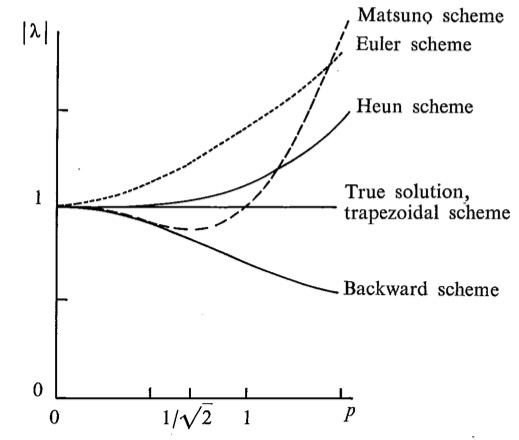
\includegraphics[keepaspectratio]{./pictest/pic5.jpg}}
\caption{}
\end{figure}

Figure \texttt{figg:5} Summarizes the results obtained for the five
schemes considered so far. For all of these schemes the amplification
factors were found to be even functions of \(p\), so the amplification
factor curves are shown only for \(p \geq 0\).

It is also of interest to consider the phase change per time step,
\(\theta\) and the relative phase change per time step, \(\theta p\).

Using the notation

{\[\lambda \equiv \lambda_{\text{re}} + i\lambda_{im}\]}

we have, using \texttt{h2.4},

{\[\theta = \arctan\frac{\lambda_{\text{im}}}{\lambda_{\text{re}}}\]}

or

{\[\frac{\theta}{p} = \frac{1}{p}\arctan\frac{\lambda_{\text{im}}}{\lambda_{\text{re}}}\]}

For the Euler and the backward schemes, using \texttt{h2.11} and
\texttt{h2.12} we obtain

{\[\frac{\theta}{p} = \frac{1}{p}\arctan\text{p}\]}

Since the right-hand side is always less than unity, we can see that
these two schemes are decelerating. For \(p = 1\) we have
\(\theta p = \pi 4\).

In other cases the effect may not be so obvious. For the Matsuno scheme,
for example, \texttt{h2.21} gives

{\[\frac{\theta}{p} = \frac{1}{p}\arctan\frac{p}{1 - p^{2}}\]}

It is not obvious whether the right-hand side here is greater or less
than unity. However, the behaviour of \texttt{h2.31} for all \(p\) is of
no practical interest, since we already know that \(p`must be chosen
less than unity in order to ensure stability, and rather small for
frequencies for which we want the integration errors to be small. Thus,
we need only consider :eq:`h2.31\) for small \(p\); we obtain

\[\frac{\theta}{p} = 1 + \frac{2}{3}p^{2} + \ldots\]

The Matsuno scheme, therefore, is seen to be accelerating. For the
special value \(p = 1\) this can be seen directly from \texttt{h2.13},
since then \(\frac{\theta}{p} = \frac{\pi}{2}\).

Analysis of phase errors of schemes applied to the oscillation equation
is not so important as analysis of the amplification factor. Phase
errors do not affect stability, and when these schemes are used to solve
the partial differential equations of motion additional phase errors due
to space differencing will appear. We will then be interested only in
the total phase error, and it will be found that the error due to space
differencing is usually dominant.

\subsubsection{Three level schemes and computational
modes}\label{three-level-schemes-and-computational-modes}

We consider first the leapfrog scheme \texttt{h1.9}. Applied to the
oscillation equation it gives

{\[U^{n + 1} = U^{( n + 1 )} + i 2\omega\Delta U^{\left( n \right)}\]}

A problem with all three or more level schemes includ­ing this is that
they require more than one initial condition to start the computation.
From a physical standpoint a single initial condition
\(U^{\left( 0 \right)}\) should have been sufficient. However, in
addition to the physical initial condition, three level schemes require
a computational initial condi­tion \(U^{\left( 1 \right)}\)). This value
cannot be calculated by a three level scheme, and, therefore, it will
usually have to be obtained using one of the two level schemes.

According to \texttt{h2.3} we also have

{\[U^{\left( n \right)} = \lambda U^{\left( n - 1 \right)},
U^{\left( n + 1 \right)} = \lambda^{2}U^{\left( n - 1 \right)}\]}

When these relations are substituted into \texttt{h2.32} we obtain

\[\lambda^{2} - i2p\lambda - 1 = 0\]

a second degree equation for \(\lambda\). It has solutions

{\[\lambda_{1} &= \sqrt{1 + p^{2}} + i p\]\[\lambda_{2} &= - \sqrt{1 - p^{2}} + i p\]}

Thus, there are \emph{two solutions} of the form
\(U^{n + 1} = \lambda U^{( n )}\). This necessarily follows from the
fact that we are consider­ing a three level scheme; substitution of
\texttt{h2.33} into the difference equation given by these schemes will
always give a second degree equation for \(\lambda\). In general, an
\emph{m} level scheme will give \emph{m — 1} solutions of the form
\(U^{n + 1} = \lambda U^{\left( n \right)}\). A solution of this type
corresponding to a single value of \(\lambda\) is called a \emph{mode}.

Consider now the two values that have been obtained for \(\lambda\). If
a solution of the form \(U^{n + 1} = \lambda U^{\left( n \right)}\) is
to represent an approximation to the true solution, then we must have
\(\lambda \rightarrow 1\) as \(\Delta \rightarrow 0\). For the values
\texttt{h2.34}, as \(p \equiv \omega\Delta t \rightarrow 0\) we do have
\(\lambda_{1} \rightarrow 1\), however at the same time
\(\lambda_{2} \rightarrow - 1\). Solutions like that associated with
\(\lambda_{2}\) are usually called \emph{physical modes} because we are
always solving equations describing physical processes. Solu­tions like
that associated with \(\lambda_2\) are not approximations to the true
solution, and are called \emph{computational modes}.

To clarify this situation we consider the simple case \(\omega = 0\),
that is, the equation

{\[\frac{d U}{d t} = 0\]}

with the true solution

{\[U = const\]}

The leapfrog scheme, applied to \texttt{h2.35}, gives

{\[U^{\left( n + 1 \right)} = U^{\left( n - 1 \right)}\]}

For a given physical initial condition \(U^{\left( 0 \right)}\), we
consider two special choices of \(U^{\left( 1 \right)}\).

A. Suppose calculating of \(U^{\left( 1 \right)}\) happened to give the
true value \(\text{U}^{\left( 0 \right)}\), \texttt{h2.37} then gives,
for all n,

\[U^{\left( n + 1 \right)} = U^{\left( n \right)}\]

or, since p = 0,

\[U^{\left( n + 1 \right)} = \lambda_{1}U^{\left( n \right)}\]

Thus, we obtain a numerical solution that is equal to the true solution
\texttt{h2.36}, and consists of the physical mode only.

B. Suppose calculating \(U^{\left( 1 \right)}\) gives
\(U^{\left( 1 \right)} = - U^{\left( 0 \right)}\).

Then we obtain, for all n,

\[U^{\left( n + 1 \right)} = - U^{\left( n \right)}\]

or

\[U^{\left( n + 1 \right)} = \lambda_{2}U^{\left( n \right)}\]

The numerical solution now consists entirely of the computational mode.
Hence, it would appear that a good choice of the computational initial
condition is of vital importance for obtaining a satisfactory numerical
solution.

In general, since \texttt{h2.31} is a linear equation, its solution will
be a linear combination of the two solutions

\[U_{1}^{\left( n \right)} &= \lambda_{1}^{n}U_{1}^{\left( 0 \right)}\]\[U_{2}^{\left( n \right)} &= \lambda_{2}^{n}U_{2}^{\left( 0 \right)}\]

Therefore, we can write

{\[U^{\left( n \right)} = a\lambda_{1}^{n}U_{1}^{\left| 0 \right|} + b\lambda_{2}^{n}U_{2}^{\left( 0 \right)}\]}

where a and b are constants. Now this has to satisfy the physical and
the computational initial condition; we obtain

\[U^{\left( 0 \right)} = a U_{1}^{\left| 0 \right|} + b U_{2}^{\left( 0 \right)}\]\[U^{\left( 1 \right)} = a\lambda_{1}U_{1}^{\left( 0 \right)} + b U_{2}^{\left( 0 \right)}\]

These equations can be solved for a \(U_{1}^{\left( 0 \right)}\) and
\(bU_{2}^{\left( 0 \right)}\), and the results substituted into
\texttt{h2.38}.

In this way we find

{\[U^{(n)} = \frac{1}{\lambda_1 - \lambda_2} \left[ \lambda_1^n\left( U^{(1)}
 - \lambda_{2}U^{(0)} \right) - \lambda_2^n\left( U^1 - \lambda_{1}U^{(0)} \right) \right]\]}

Therefore, the amplitudes of the physical and of the computational modes
are seen to be proportional to, respectively,

\[|U^{(1)} - \lambda_2 U^{(0)}| \quad   and   \quad | U^{(1)} - \lambda_1 U^{(0)} |\]

These are seen to depend on \(U^{\left( 1 \right)}\). If, for example,
we are able to choose
\(U^{\left( 1 \right)} = \lambda_{1}U_{1}^{\left( 0 \right)}\), the
numerical solution will consist of the physical mode only. If, on the
other hand, the choice of \(U^{\left( 1 \right)}\) is so unsuccessful as
to have \(U^{\left( 1 \right)} = \lambda_{2}U^{\left( 0 \right)}\), the
solution will consist entirely of the computational mode.

While this analysis illustrates the importance of a careful choice of
\(\text{U}^{\left( 1 \right)}\), it is not always possible to calculate
\(U^{\left( 1 \right)} = \lambda_{1}U^{\left( 0 \right)}\) so as to
eliminate the computational mode. Numerical methods are used in practice
to solve equations that cannot be solved by analytical methods, and are
more complex than the simple oscillation equa­tion \texttt{h2.1}. In
these cases we will not know the exact values of \(\lambda_{1}\) and
\(\lambda_{2}\).

Thus \(U^{\left( 1 \right)}\),, is usually computed using one of the two
level schemes. The simplest method is to use the Euler scheme, or, a
more refined procedure could be used, for example the Heun scheme. Using
\texttt{h2.39} it can be shown that the latter alternative will give a
smaller amplitude of the computational mode.

We also note that even if we did know the exact value of \(\lambda_{1}\)
this would still not allow the computational mode to be eliminated in a
practical numerical calculation. The numerical solution which we
calculate is not an exact solution of the finite difference equations,
since the arithmetical operations are performed in practice only to a
finite number of significant digits. The error produced in this way is
called \emph{round off error}, though in electronic computers results of
arithmetic operations are sometimes truncated to a given number of
digits, instead of being rounded off. With round off errors present,
permanent elimination of the computational mode is not possible in
principle, since the computational mode would appear in the course of
integration in any case even if were absent initially. However, it is
usually found that round off errors are of little importance in
atmospheric models, and in solving partial differential equations in
general.

Proceeding now to the stability analysis, in view of \texttt{h2.38} and
our inability to eliminate the computational mode completely, we will
have to require for stability that neither of the two amplification
factors is greater than unity. It is convenient to consider three
special cases.

\paragraph{\texorpdfstring{\(\left| p \right| \leq 1.\)}{\textbackslash left\textbar{} p \textbackslash right\textbar{} \textbackslash leq 1.}}\label{left-p-right-leq-1.}

In \texttt{h2.34} \(1 - p^{2}\) is positive, and we obtain
\(\left| \lambda_{1} \right| = \left| \lambda_{2} \right| = 1\)

Thus, in this case both modes are stable and neutral. For the phase
change, using \texttt{h2.28}

{\[\theta_{1} = arctan\left( \frac{p}{\sqrt{1 - p^{2}}} \right)\]}

\[\theta_{2} = arctan\left( \frac{- p}{\sqrt{1 - p^{2}}} \right)\]

It is instructive to consider the behaviour of \(\theta\), as a function
of \(p\), especially as \(p \rightarrow 0.\) We consider first the case
\(p > 0.\). Since for both modes
\(\lambda_{\text{im}} = \left| \text{λ} \right|\sin{\theta = p}`we
have :math:`0 < \theta < \pi\). Considering the signs of
\(\lambda_{\text{re}}`we find that,
:math:`0 < \theta < \frac{\pi}{2}`and
:math:\)frac\{pi\}\{2\} \textless{} t\href{}{heta}\{2\} \textless{} pi`.
To illustrate these results, the phase changes \texttt{h2.41} are
plotted in \texttt{figg:6}. We see that, for all \(p\),

\begin{figure}
\centering
\pandocbounded{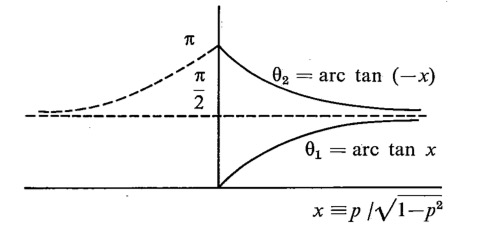
\includegraphics[keepaspectratio]{./pictest/pic6.jpg}}
\caption{}
\end{figure}

\[\theta_{2} = \pi - \theta_{1}\]

Specifically, as \(p \rightarrow 0, \theta_{1} \rightarrow p\) while
\(\theta_{2} \rightarrow \pi - p\)

Thus, for small \(\Delta t\) the physical mode is seen to approximate
the true solution, while the behaviour of the computa­tional mode is
quite different. For the case \(p < 0\), we obtain in the same way

\[\pm \theta_{2} = - \pi - \theta_{1}\]

Thus, for \(p \gtrless 0\)

{\[\theta_{2} = \pm \pi - \theta_{1}\]}

For accuracy of the physical mode, \(\theta_{1}\) should closely
approximate the phase change of the true solution, \emph{p}. For small
\emph{p} \texttt{h2.41} gives

\[\theta_{1} = p + \frac{1}{6}p^{3} + \ldots\]

Thus, the leapfrog scheme is accelerating. The accelera­tion, though, is
four times less than that of the Matsuno scheme. It is instructive to
note that schemes of different orders of accuracy can still have the
same order of leading term in power series expansions of either the
amplification factors or the phase changes.

Differentiating the first equation in \texttt{h2.41} we find

\[\frac{d\theta_{1}}{\text{dp}} = \frac{1}{\sqrt{1 - p^{2}}}\]

The phase error, thus, is seen to increase sharply as
\(p \rightarrow 1.\), when
\(\frac{\theta_{1}}{p} \rightarrow \frac{\pi}{2}\)

It may be useful to illustrate the behavior of the two modes obtained

{\[U_{1}^{\left( n \right)} &= U_{1}^{\left( 0 \right)}e^{in\theta 1}\]\[U_{2}^{\left( n \right)} &= U_{2}^{\left| 0 \right|}e^{\text{in}\left( \pm \pi - \theta_{1} \right)}\]}

in the complex plane. For simplicity, we consider the case
\(\theta_{1} = \frac{\pi}{8}\) and assume that the imaginary part of the
solution is equal to zero at the initial moment. The physical mode, as
seen in \texttt{h2.43}, rotates in the positive sense by an angle
\(\theta_{1}\) in each time step \(\Delta t\), while at the same time
the computational mode, in the case \emph{p \textgreater{} 0}, rotates
by an angle \(\pi - \theta_{1}\). Therefore, the two modes can be
represented graphically as in \texttt{figg:7}.

\begin{figure}
\centering
\pandocbounded{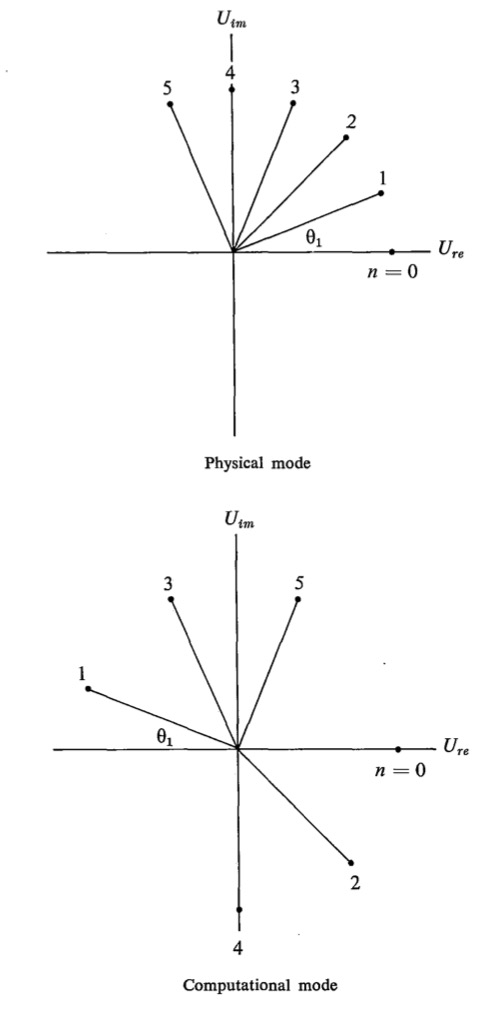
\includegraphics[keepaspectratio]{./pictest/pic7.jpg}}
\caption{}
\end{figure}

A detailed knowledge of the behaviour of the computa­tional mode may be
helpful in recognizing its excessive presence in an integration. Thus,
we plot the real and imaginary parts of the computational mode as
functions of time. This can be done by using an alternative form of the
second equation in \texttt{h2.43}

\[U_{2}^{\left( n \right)} = {\left( - 1 \right)^{n}U}_{2}^{\left( 0 \right)}\left( \cos{n\theta_{1}} - i\sin{n\theta_{2}} \right)\]

or directly from \texttt{figg:7}. We obtain diagrams as shown in
\texttt{figg:8}. Because of the factor (—1)", both real and imaginary
parts oscillate between time steps.

\begin{figure}
\centering
\pandocbounded{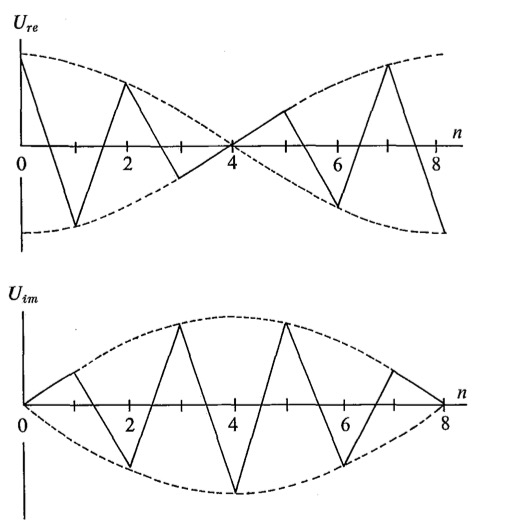
\includegraphics[keepaspectratio]{./pictest/pic8.jpg}}
\caption{}
\end{figure}

\paragraph{\texorpdfstring{\(\left| p \right| = 1\)}{\textbackslash left\textbar{} p \textbackslash right\textbar{} = 1}}\label{left-p-right-1}

This is a limiting case of the solutions considered for
\(\left| \text{p} \right| < 1\). \texttt{h2.34} shows that the values of
\(\lambda\). are now equal,

{\[\lambda_{1} = 2 = ip\]}

Therefore

\[\left| \lambda_{1} \right| = \left| \lambda_{2} \right| = 1\]

Thus, both modes are still neutral. Since neither of them has a real
part, we obtain, for p = ± 1,

{\[\theta_{1} = \theta_{2} = \pm \frac{\pi}{2}\]}

Therefore, the two modes can be written in the form

{\[U^{\left( n \right)} = U^{\left( 0 \right)}e^{\pm i n\frac{\pi}{2}}\]}

In a complex plane, they rotate by an angle of \(\frac{\pm \pi}{2}\) in
each time step, while the true solution rotates by an angle of ± 1
only. The phase error, thus, is large.

\paragraph{\texorpdfstring{\(\left| p \right| > 1\)}{\textbackslash left\textbar{} p \textbackslash right\textbar{} \textgreater{} 1}}\label{left-p-right-1-1}

Both values of \(\lambda\) in \texttt{h2.34} still have imaginary parts
only, so that

\[\lambda_{1} &= i\left( p + \sqrt{p^{2}} - 1 \right)\]\[\lambda_{2} &= i\left( p - \sqrt{p^{2} - 1} \right)\]

where the expressions in parentheses are real. Therefore,

{\[\left| \lambda_{1} \right| = \left| p + \sqrt{p^{2}} - 1 \right|\]\[\left| \lambda_{2} \right| = \left| p - \sqrt{p^{2}} - 1 \right|\]}

Thus, for \emph{p \textgreater{} 1} we have
\(\left| \lambda_{1} \right| > 1\), and for \emph{p \textless{} — 1}
\(\left| \lambda_{2} > 1 \right|\). Therefore, for
\(\left| p > 1 \right|\) the leapfrog scheme is unstable. The
instability increases sharply as \(\left| \text{p} \right|\) increases
beyond 1 ; we can see this, for example for \emph{p \textgreater{} 1},
because

\[\frac{d\left| \lambda \right|_{1}}{\text{dp}} = 1 + \frac{p}{\sqrt{p^{2}} - 1}\]

which is unbounded as \(p \rightarrow 1\)

Since the two values of \(\lambda\) still have no real parts, we again
have

{\[\theta_{1} = \theta_{2} = \pm \frac{\pi}{2}\]}

The two modes for \(p \gtrless 1\), can thus be written as

{\[U_{1}^{\left( n \right)} &= \left| p + \sqrt{p^{2} - 1} \right|^{n}U_{1}^{\left( 0 \right)}e^{\pm in\frac{\pi}{2}}\]\[U_{2}^{\left( n \right)} &= \left| p - \sqrt{p^{2} - 1} \right|^{n}U_{2}^{\left( 0 \right)}e^{\pm in\frac{\pi}{2}}\]}

In the complex plane, both modes again rotate by an angle of
\(\frac{\pm \pi}{2}\) in each time step. However, this time the
amplitude of one of the modes increases, and that of the other decreases
with time. The real part of the unstable mode can, for instance, be
represented as a function of time by a graph like that in Fig. 2.5.
Because of \texttt{h2.48} the period of the unstable oscillation is
always \(4\Delta t\). This can be used to diagnose the instability: if
the results appear unsatisfactory, it is a good idea to

check for the presence of growing oscillations of that period.

\begin{figure}
\centering
\pandocbounded{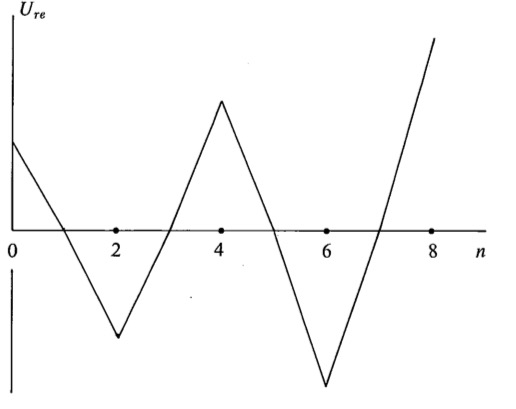
\includegraphics[keepaspectratio]{./pictest/pic9.jpg}}
\caption{}
\end{figure}

To sum up, advantages of the leapfrog scheme are that it is a very
simple scheme, of second order accuracy, and neutral within the
stability range \(\left| \omega\Delta t \leq 1 \right|\). A disadvantage
of the leapfrog scheme is the presence of a neutral computational mode.
With nonlinear equations there is a tendency for a slow amplification of
the compu­tational mode. An example of this growth can be seen, for
example, in one figure of a paper by Lilly (1965). The usual method used
for suppressing this instability is the occasional insertion of a step
made by a two level scheme, which eliminates the computational mode. A
multi-level scheme that damps the computational mode could also be used
for this purpose.

When solving the system of gravity wave equations, as will be shown in
Chapter \texttt{Chapter4}, it is possible to construct grids and/or
finite difference schemes which have essen­tially the same properties as
the leapfrog scheme, but in which the computational mode is absent.
These methods calculate the physical mode only, and at the same time
require only one half of the computation time needed for the regular
leapfrog scheme as described here.

We consider, finally, stability and other properties of the
Adams-Bashforth scheme \texttt{h1.10}. Applied to the oscillation
equation it gives

{\[U^{( n + 1 )} = U^{(n)} + i\omega\Delta t \left( \frac{3}{2}U^{( n )} - \frac{1}{2}U^{\left( n - 1 \right)} \right)\]}

Substituting the relations \texttt{h2.33} we find

\[\lambda^{2} - \left( 1 + i\frac{3}{2}p \right)\lambda + i\frac{1}{2}p = 0\]

We have, of course, again obtained a second degree equation for
\(\lambda\).

It has the solutions

{\[\lambda_{1} = \frac{1}{2}\left( 1 + i\frac{3}{2}p + \sqrt{1 - \frac{9}{4}p^{2} + ip} \right)\]\[\lambda_{2} = \frac{1}{2}\left( 1 + i\frac{3}{2}p - \sqrt{1 - \frac{9}{4}}p^{2} + ip \right)\]}

Thus, as \(p \rightarrow 0\), \(\lambda_{1} \rightarrow 1 \) while
\(\lambda_{2} \rightarrow 0\). We see that the solution associated with
\(\lambda_{2}\) again represents a physical mode, and that associated
with \(\lambda_{2}\) a computational mode. However, while for the
leapfrog scheme the computational mode was found to be neutral, here it
is seen to be damped. This is a very useful property of the
Adams-Bashforth scheme as the computational mode cannot cause
inconveniences.

The exact analysis of the amplification factors here is more difficult
because of the presence of square roots in \texttt{h2.51}. However,
since for reasons of accuracy we have to choose a relatively small value
of p in any case, it will suffice to consider amplification factors for
small values of p only. The power series expansion of \texttt{h2.51}
then gives

\[\lambda_{1} = 1 + ip - \frac{1}{2}p^{2} + i\frac{1}{4}p^{3} - \frac{1}{8}p^{4} + \ldots\]\[\lambda_{2} = i\frac{1}{2}p^{2} + i\frac{1}{2}p^{2} - \frac{1}{4}p^{3} + \frac{1}{8}p^{4}\ldots\]

Now, after rearranging the terms these series can be written as

\[\lambda_{1} = \left( 1 - \frac{1}{2}p^{2} - \frac{1}{8}p^{4} - \ldots \right) + i\left( p + \frac{1}{4}p^{3} + \ldots \right)\]\[\lambda_{2} = \left( \frac{1}{2}p^{2} + \frac{1}{8}p^{4} + \ldots \right) + i\left( \frac{1}{2}p - \frac{1}{4}p^{3} - \ldots \right)\]

which can be used to obtain the amplification factors

{\[\left| \lambda_{1} \right| &= \left( 1 + \frac{1}{2}p^{4} + \ldots \right)^{\frac{1}{2}}\]\[\left| \lambda_{2} \right| &= \left( \frac{1}{4}p^{2} + \ldots \right)^{\frac{1}{2}}\]}

The higher order terms have been omitted. A final expansion gives

{\[\left| \lambda_{1} \right| &= 1 + \frac{1}{4}p^{4} + \ldots\]\[\left| \lambda_{2} \right| &= \frac{1}{2}p + \ldots\]}

Expressions \texttt{h2.52} and/or \texttt{h2.53} show that the physical
mode of the Adams-Bashforth scheme is always unstable. However, as for
the Heun scheme, the amplification is only by a fourth order term, and
it can be tolerated when a sufficiently small value of \(\Delta t\) is
chosen. Note that the amplification given by \texttt{h2.53} is twice
that given by \texttt{h2.26} for the Heun scheme. Since the
amplification is propor­tional to \(\left( \Delta t \right)^{4}\),
however, a small reduction in time step would compensate for that
difference. Thus, the Adams-Bashforth scheme, with only one evaluation
of the right hand side per time step, can still be considered much more
economical. It has been fairly frequently used in meteorological
numerical studies. For example, it is being used by Deardorff in his
numerical simulations of the planetary boundary layer (e.g. Deardorff,
1974).

Analyses of the properties of some other schemes, applied to the
oscillation equation, can be found in papers by Lilly (1965), Kurihara
(1965) and Young (1968). In practice the choice of a scheme will depend
not only on the properties considered here, but also on some practical
considerations. For example, we might expect that the three level
schemes, since they use more informa­tion, would generally give better
results than the two level schemes. Our findings agree with that
conjecture ; for example, for second order accuracy the explicit three
level schemes required only one evaluation of the right hand side per
time step, while the two level schemes required two evaluations. As
another example, if we want to damp high frequency motions with three
level schemes we can linearly extrapolate the derivative beyond the
centre of the interval
\(\left( n\Delta t,\left( n + 1 \right)\Delta t \right)\), and thus
obtain a scheme that will perform such a damping in a more selective and
more economical way than the Mat-suno scheme (Mesinger, 1971). However,
three level schemes generally require more core storage space in the
computer than two level schemes and this may affect our our decision.

\subsection{\texorpdfstring{\textbf{Properties of schemes applied to the
friction
equation}}{Properties of schemes applied to the friction equation}}\label{properties-of-schemes-applied-to-the-friction-equation}

We shall now consider the properties of schemes when applied to the
equation

{\[\frac{d U}{d t} = - \kappa U, \qquad U = U\left( t \right), \qquad \kappa > 0\]}

We shall call this equation the friction equation.

Again it is easy to justify our interest in this equation. For example,
if we define \(U \equiv u + iv\), it describes the effect of friction
proportional to the velocity vector, as is often assumed for motions
near the ground. As another example, note that when seeking a solution
of the heat transfer, or Fick\textquotesingle s diffusion equation

\[\frac{\partial u}{\partial t} = \sigma\frac{\partial^{2} u }{{\partial x}^{2}}, \qquad \sigma > 0\]

in the form of a single harmonic component

\[u\left( x,t \right) = Re\left\lbrack \left( U\left( t \right)e^{\text{ikx}} \right) \right\rbrack\]

we obtain

\[\frac{\text{dU}}{\text{dt}} = - \sigma k^{2}U\]

\begin{description}
\item[This is equivalent to \texttt{k3.1} if we substitute]
\(x \equiv \sigma k^{2}\).
\end{description}

The general solution of \texttt{k3.1} is

{\[U\left( t \right) = U\left( 0 \right)e^{- \kappa t}\]}

Thus, both the real and the imaginary part decrease exponentially with
time.

The properties of schemes applied to \texttt{k3.1} will again be
analyzed using the von Neumann method. As in the previous section, we
consider first the non-iterative two level scheme \texttt{h2.6}. Applied
to the friction equation, \texttt{h2.6} gives

{\[U^{(n + 1)} = U^{n} - \kappa\Delta t \left( \alpha U^{( n )} + \beta U^{\left( n + 1 \right)} \right)\]}

Writing

{\[K \equiv \kappa \Delta t\]}

we obtain, rearranging the terms in \texttt{k3.3},

{\[U^{\left( n + 1 \right)} = \frac{1 - \alpha K}{1 + \beta K}U^{\left( n \right)}\]}

For the Euler scheme \(\alpha = 1`and :math:\)beta = 0`; thus,
\texttt{k3.5} shows that the Euler scheme is now stable if
\(\left| 1 - K \leq 1 \right|\), that is, if

{\[0 < K \leq 2\]}

Thus we see that the stability criteria of particular schemes do not
have to be the same when they are applied to different equations. In the
case of \texttt{k3.6}, one will normally be more demanding in the choice
of \(\Delta t\). For example, we will want \emph{K \textless{} 1}, to
prevent the solution \texttt{k3.5} oscillating from time step to time
step.

For the backward scheme \(\alpha = 0`and :math:\)beta = 1`; it is always
stable if \emph{K \textgreater{} 0}. The solution does not oscillate in
sign.

For the trapezoidal scheme \(\alpha = \frac{1}{2}`and
:math:\)beta = frac\{1\}\{2\}`; the scheme is again always stable for
\emph{K \textgreater{} 0}. The solution does not oscillate if \emph{K
\textless{} 2}.

Considering the iterative two level scheme \texttt{h2.18} we obtain

{\[U^{\left( n + 1 \right)} = \left( 1 - K + \beta K^{2} \right)U^{\left( n \right)}\]}

Therefore, both the Matsuno and the Heun scheme are stable for
sufficiently small values of \emph{K}.

It is instructive to consider in some detail the behaviour of the
numerical solution obtained using the leapfrog scheme. Applied to
\texttt{k3.1} it gives

{\[U^{\left( n + 1 \right)} = U^{\left( n - 1 \right)} - 2\Delta t U^{\left( n \right)}\]}

The equation for the amplification factor is

\[\lambda^{2} + 2K\lambda - 1 = 0\]

giving the solutions

{\[\lambda_{1} = - K + \sqrt{1 + K^{2}}\]\[\lambda_{2} = - K - \sqrt{1 + K^{2}}\]}

As \(k \rightarrow 0, \quad \lambda \rightarrow 1,\) while
\(\lambda_{2} \rightarrow - 1\) thus, the solution associated with
\(\lambda_{1}\) again represents the physical mode, and that associated
with \(\lambda_{2}\) the computational mode. For \emph{K \textgreater{}
0}, that is, for the normal case of a forward integration in time, we
have \(\lambda_{2} < - 1\); hence, the compu­tational mode is always
unstable. It changes sign from time step to time step, and its magnitude
increases. As before, we cannot hope to eliminate the computa­tional
mode completely. This amplification is not negligible, and the leapfrog
scheme is therefore not suitable for numerical integration of the
friction equation.

A simple example can be given to illustrate the in­stability of the
leapfrog scheme. Let U have only a real part, and suppose we have set
\(U^{( 1 )} = U^{( 0 )}\), as shown in \texttt{figg:10} Furthermore, let
the dashed curve in the figure represent the true solution satisfying
the given initial condition \(U^{\left( 0 \right)}\). Knowing
\(U^{\left( 0 \right)}\), \(U^{\left( 1 \right)}\), and the true
solution it is possible to construct a graph of the numerical solution,
using the fact that \(\frac{\text{dU}}{dt = - \kappa U}\) is equal to
the slope of the line tangent to the true solution at the appro­priate
value of U. In this way we obtain the numerical solution shown by the
full line. In this method, the deri­vative is calculated as a function
of the current value of \(U^{\left( n \right)}\), and the increment due
to this derivative is added to the preceding value. This is seen to
result in an unbounded growth of the difference between consecutive
values of \(U^{\left( n \right)}\), even when this difference is equal
to zero initially.

\begin{figure}
\centering
\pandocbounded{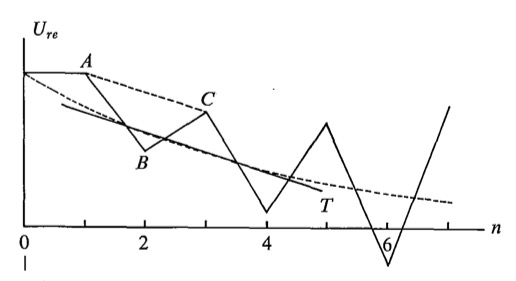
\includegraphics[keepaspectratio]{./pictest/pic10.jpg}}
\caption{}
\end{figure}

Finally, for the Adams-Bashforth scheme we obtain

{\[\lambda = \frac{1}{2}\left( 1 - \frac{3}{2}K \pm \sqrt{1 - K\frac{9}{4}K^{2}} \right)\]}

The Adams-Bashforth scheme, thus, is stable for suffi­ciently small
values of K. The computational mode is damped.

\subsection{\texorpdfstring{\textbf{A combination of
schemes}}{A combination of schemes}}\label{a-combination-of-schemes}

A natural question to ask at this point is what can we do if, for
example, the equation contains both the oscilla­tion and the friction
term, that is

{\[\frac{\text{dU}}{\text{Dt}} = i\omega U - \kappa U\]}

Here we might like to use the leapfrog scheme because of the oscillation
term \(i\omega U\), but we know that it cannot be used for the friction
term \(- \kappa U\). In this and similar situations we can use different
schemes for the different terms; for example, we might use the leapfrog
scheme for the oscillation term and the forward scheme for the friction
term. We then obtain

\[U^{\left( n + 1 \right)} = U^{\left( n - 1 \right)} + 2\Delta t\left( i\omega U^{\left( n \right)} - \kappa U^{\left( n - 1 \right)} \right)\]

Other combinations, of course, are also possible.

\section{The Advection Equation}\label{Chapter3}

We now consider differential equations with one dependent and two or
three independent variables, that is, partial differential equations.
More specifically, we shall consider various simplified forms of the
advection equation, describing advection of a dependent variable. This
is considered in practice to be the most important part of the
atmospheric governing equations.

We have already discussed the one-dimensional linear advection equation
to some extent in the introductory chapter. We shall organize the
analysis here so as first to continue considering problems associated
with the simplest one-dimensional linear form of the advection equation,
and then to proceed to problems introduced by more complex forms of the
advection equation.

\subsection{\texorpdfstring{\textbf{Schemes with centered second-order
space
differencing}}{Schemes with centered second-order space differencing}}\label{Section3.1}

We shall first consider the equation

{\[\frac{\partial u}{\partial t}  +c\frac{\partial u}{\partial x} = 0\]\[c = const.\]}

Here \(u = u\left( x,t \right)\) is a function of two independent
varia­bles : the independent variable \(x\) will represent a space
variable, and, thus, \texttt{a1.1} will be called the one-dimen­sional
linear advection equation. As seen earlier, its general solution is

{\[u = f\left( x - ct \right)\]}

where \(f\) is an arbitrary function. The name \emph{advection equation}
was suggested by Phillips (1960).

One of the finite difference schemes for \texttt{a1.1} is the forward
and upstream scheme, which has been shown excessively damping in the
Chapter \texttt{Chapter1} .

If the space derivative in \texttt{a1.1} is approximated by a centered
finite difference quotient using values at the two nearest points, we
obtain for the time derivative

{\[\frac{\partial u_{j}}{\partial t} = - c\frac{u_{j + 1} - u_{j - 1}}{2\Delta x}\]}

The subscript here, as before, denotes the distance from the origin in
space increments; that is, \(x = j\Delta x\). A number of schemes for
the numerical solution of \texttt{a1.1} can now be constructed because
we can approximate the time derivative in \texttt{a1.3} by one of the
methods studied in the preceding chapter. For example, when the time
derivative is approximated using the leapfrog scheme, we obtain

{\[\frac{u_{j}^{n + 1} - u_{j}^{n - 1}}{2\Delta t} = - c\frac{u_{j + 1}^n - u_{j - 1}^n}{2\Delta x}\]}

as one of many possible consistent schemes for the numerical solution of
\texttt{a1.1}.

The properties of schemes constructed in this way can be inferred from
the known properties of time differencing schemes applied to the
oscillation equation. To see this, we substitute into \texttt{a1.3} a
tentative solution in form of the single harmonic component

{\[u_{j} = Re\left\lbrack U\left( t \right)e^{ikj\Delta x} \right\rbrack\]}

After some rearrangement, this gives

{\[\frac{\text{dU}}{\text{dt}} = i\left( - \frac{c}{\Delta t}\sin{k\Delta x} \right)U\]}

If we denote

{\[\omega \equiv - \frac{C}{\Delta x}\sin{k\Delta x}\]}

this is equivalent to the oscillation equation of the previous chapter.
Now, if we approximate \texttt{a1.6} using one of the time differencing
schemes studied in that chapter, the same finite difference equation is
obtained as when we apply that scheme to \texttt{a1.3} and then
substitute the wave solution \texttt{a1.5}. Hence, properties of finite
difference schemes derived from \texttt{a1.3} can be inferred from the
results of Section \texttt{Section2.1}, where the frequency to is given
by \texttt{a1.7}.

As an example, if \texttt{a1.6} is approximated using the leapfrog
scheme, we obtain

{\[U^{\left( n + 1 \right)} = U^{\left( n - 1 \right)} + 2\left( - c\frac{\Delta t}{\Delta x}\sin{k\Delta x} \right)U^{\left( n \right)}\]}

Using the notation of chapter \texttt{Chapter2}, we write

{\[p = - c\frac{\Delta t}{\Delta x}\sin{k\Delta x}\]}

We obtain the same finite difference equation \texttt{a1.8} by first
applying the leapfrog scheme to \texttt{a1.3} giving \texttt{a1.4} and
then substituting \texttt{a1.5} into \texttt{a1.4}. Thus, properties of
\texttt{a1.4} can be inferred from (1.7) and from the known properties
of the leapfrog scheme applied to the oscillation equation.

Let us look at some of conclusions obtained in this way. For stability
of the leapfrog scheme it was required that the condition
\(\left| p \right| \leq 1 \) │ be satisfied for all values of \(\omega\)
occuring. Thus, we have to satisfy

\[\left| c\frac{\Delta t}{\Delta x}\sin{k\Delta x } \right| \leq 1\]

for any admissible k. Since \(\left| \sin{k\Delta x} \right|\) does
reach the maximum value of unity in the admissible range of k, we obtain
the stability condition

{\[\left| c \right|\frac{\Delta t}{\Delta x} \leq 1\]}

This criterion, obtained already in the Chapter \texttt{Chapter1}, shows
that stability cannot simply be achieved by reduction of the time and
space increments. Rather, it is necessary to reduce the ratio of these
increments \(\frac{\Delta x}{\Delta t }\) to obtain stability. The
condition \texttt{a1.10} was first found by Courant, Friedrichs and Lewy
(1928), and, therefore, is usually referred to as the
Courant-Friedrichs-Lewy, or CFL, stability criterion.

It is instructive to note that the maximum value of
\(\left| p \right|\), that is, the minimum stability, is associated with
the wave with \(k\Delta x = \frac{\pi}{2}\). This is the component with
wave length 4 \(\Delta x\), twice the shortest resolvable wave length
\(2\Delta x\).

We can also use other results of the previous analysis. There are two
solutions for \(U^{\left( n \right)}\), the physical and the
computational mode

{\[U_{1}^{\left( n \right)} = \lambda_{1}^{n}U_{1}^{\left( 0 \right)}U_{2}^{\left( n \right)} 
= \lambda_{2}^{\left( n \right)}U_{2}^{\left( 0 \right)}\]}

\(\lambda_{1}\) and \(\lambda_{2 }\) are given here by Eqs.
\texttt{h2.34} of Chapter \texttt{Chapter2}. In the stable case, we
have, for \(p \gtrless 0\)

{\[\lambda_{1} = c^{i\theta}, \qquad \theta = arctan\left( \frac{p}{\sqrt{1 - p^{2}}} \right)\]}

\[\lambda_{1} = e^{i\left( \pm\pi-\theta\right)} = - e^{- i\theta}\]

Using \texttt{a1.5}, it is seen that the approximation u{]} also has a
physical and a computational mode. For the physical mode

{\[u_{j}^{n} = Re\left\lbrack U_{1}^{\left( 0 \right)}e^{\left( j\Delta x 
+ \frac{\theta}{k\Delta t}n\Delta t \right)} \right\rbrack\]}

For the computational mode, on the other hand, we obtain

{\[u_{j}^{n} = Re\left\lbrack \left( - 1 \right)^{n}U_{2}^{\left( 0 \right)}
e^{\text{ik}\left( j\Delta x - \frac{\theta}{k\Delta t} \right)} \right\rbrack\]}

These expression can be compared with the true solution of \texttt{a1.1}
in the form of a single harmonic component, as given in chapter
\texttt{Chapter1},

{\[u\left( x,t \right) = Re\left\lbrack U\left( 0 \right)e^{\text{ik}
\left( x - c t \right)} \right\rbrack\]}

We find that the phase speed of the physical mode, \(c_{1}\) is equal to
\(- \frac{\theta}{k\Delta t}\), and the phase speed of the
computa­tional mode, \(c_{2}\), considering the even time steps only, is
equal to \(\frac{\theta}{k\Delta t}\) \texttt{a1.12} shows that as
\(\Delta t \rightarrow 0, \quad \theta \rightarrow p\) and \texttt{a1.9}
shows that as
\(\Delta x \rightarrow 0, \quad p  \rightarrow \text{ck}\Delta t\).
Thus, as \(\Delta x,\Delta t \rightarrow 0, \quad c_{1} \rightarrow c\),
that is, the phase speed of the physical mode approaches the phase speed
of the true solution, while at the same time \(c_{2} \rightarrow - c\).
In addition, the compu­tational mode changes sign at all grid points
from time step to time step, because of the factor
\(\left( - 1 \right)^{n}\) in \texttt{a1.14}.

Now let us use another scheme from chapter \texttt{Chapter2} to
approximate the time derivative in \texttt{a1.3}, the Matsuno scheme.
First the approximate values \(u_{j}^{\left( n + 1 \right)^{*}}\) using
the forward scheme, that is,

{\[\frac{u_{j}^{\left( n + 1 \right)^{*}} - u_{j}^{n}}{\Delta t} 
= - c\frac{u_{j + 1}^{n} - u_{j - 1}^{n}}{2\Delta x}\]}

Then, these approximate values are used in the backward scheme, that is

{\[\frac{u_{j}^{n + 1} - u_{j}^{n}}{\Delta t} =
- c\frac{u_{j + 1}^{\left( n + 1 \right)^{*}} - u_{j - 1}^{\left( n + 1 \right)^{*}}}{2\Delta x}\]}

It is instructive to eliminate the approximate values
\(u^{\left( n + 1 \right)^{*}}\) from this equation, by substituting
values given by \texttt{a1.16}, with the subscript \(j\) replaced by
\(j + 1\) and then by \( j - 1\). In this way we obtain

{\[\frac{u_{j}^{n + 1} - u_{j}^{n}}{\Delta t} =
- c\frac{u_{j + 1}^{n} - u_{j - 1}^{n}}{2\Delta x} +
c^{2}\Delta t\frac{u_{j + 2}^{n} - 
{2u}_{j}^{n} + u_{j - 2}^{n}}{\left( 2\Delta x \right)^{2}}\]}

Without the last term, this represents the finite difference equation
obtained when the forward scheme is used for the time derivative in
\texttt{a1.3}. The third term approaches zero as
\(\Delta x,\Delta t \rightarrow 0\), and \texttt{a1.18} is therefore
also a con­sistent scheme for the advection equation. On the other hand,
for a fixed \(\Delta t\) this term approaches
\(c^{2}\Delta t\left( \frac{\partial^{2}u}{\partial x^{2}} \right)\) as
\(\Delta x \rightarrow 0\). It is therefore of the same form as a finite
difference approximation to a Fick\textquotesingle s diffusion term,

and it has a damping effect. This damping effect, how­ever, is dependent
on the wave length. As the third term is calculated over an interval of
\(4\Delta x\), the maximum damping occurs for a wave with wave length of
\(4\Delta x\). There is no damping of the shortest resolvable wave with
wave length \(2\Delta x\). Even if a damping effect were desir­able when
solving the advection equation, we would not want this particular
dependence on wave length. Thus, the Matsuno scheme does not appear
suitable for solving the advection equation.

It is convenient to include here one more example of the use of the
energy method for testing stability. In addition to being applicable
also to nonlinear equations, it can be used to study the effect of
boundary conditions on stability. We will use the energy method here to
test the stability of a group of schemes that can be used for solving
\texttt{a1.3}.

A fairly wide class of schemes for solving \texttt{a1.3} can be written
as

{\[u_{j}^{n + 1} - u_{j}^{n} = - \frac{1}{2}\mu\left( {u^{*}}_{j + 1} - {u^{*}}_{j - 1} \right)\]}

where

{\[\mu \equiv \frac{c\Delta t}{\Delta x}\]}

\begin{description}
\item[and \({u^{*}}_{j}\) is a linear function of a number of values]
\(u_{j}^{n}\)
\end{description}

For example, to obtain the non-iterative two level schemes we write

{\[{u^{*}}_{j} = \alpha u_{j}^{n} + \beta u_{j}^{n + 1}\]}

For the interative two level shemes write

{\[{u^{*}}_{j} = u_{j}^{n} - \frac{\beta}{2}\mu\left( u_{j + 1}^{n} - u_{j - 1}^{n} \right)\]}

Finally, for the Adams-Bashforthsheme

{\[{u^{*}}_{j} = \frac{3}{2}u_{j}^{n} - \frac{1}{2}u_{j}^{n - 1}\]}

Here we shall analyze the stability of the non-iterative two level
schemes. It is convenient first to multiply (1.19) by \(u_{j}\) and sum
for all \(j\); we obtain

\[\sum_{j}{u^{*}}_{j}\left( u_{j}^{n + 1} - u_{j}^{n} \right) = - \frac{1}{2}\mu\sum_{j}u^{*}_{j}\left( u^{*}_{j+1} - u^{*}_{j - 1} \right)\]

The right hand side vanished if cycle boundary conditions are assumed ;
we then have

\[\sum_{j}u^{*}_{j}\left( u_{j}^{n + 1} - u_{j}^{n} \right) = 0\]

Adding this to the relation gives

\[\sum_{j}\frac{1}{2}\left\lbrack \left( u_{j}^{n + 1} \right)^{2} - \left( u_{j}^{n} \right)^{2} \right\rbrack = \sum_{j}\frac{1}{2}\left( u_{j}^{n + 1} + u_{j}^{n} \right)\left( u_{j}^{n + 1} - u_{j}^{n} \right)\]

\begin{description}
\item[Substituting \texttt{a1.21}, and eliminating \(\beta\) using]
\(\beta = 1 - a\),
\end{description}

We obtain, after some rearrangement

{\[\sum_{j}\frac{1}{2}\left\lbrack 
\left( u_{j}^{n + 1} \right)^{2} - \left( u_{j}^{n} \right)^{2} \right\rbrack 
= \left( \alpha - \frac{1}{2} \right)\sum_{j}\left( u_{j}^{n + 1} - u_{j}^{n} \right)^{2}\]}

Thus, if \(\alpha > \frac{1}{2}\) we have anunstablescheme ; if
\(\alpha > \frac{1}{2}\) a stable and neutral scheme, and if
\(\alpha > \frac{1}{2}\) a stable and damping scheme, which makes the
total “energy” \(\sum_{j}\frac{1}{2}\left( u_{j}^{n} \right)^{2}\)
monotonically decrease with time.

Finally in this section, we shall analyze a scheme that was proposed by
Lax and Wendroff (1960) and is thus called the Lax-Wendroff scheme, or,
more specifically, the two-step Lax-Wendroff scheme. In contrast with
the schemes discussed so far, the Lax-Wendroff scheme cannot be
constructed by an independent choice of finite difference approximations
to the space and to the time derivative of the advection equation. To
describe the procedure, we use the stencil shown in \texttt{figg:11}.
First,

\begin{figure}
\centering
\pandocbounded{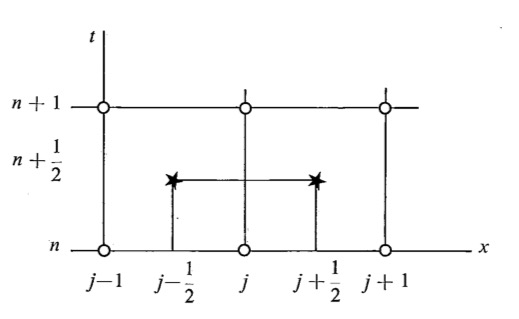
\includegraphics[keepaspectratio]{./pictest/pic11.jpg}}
\caption{}
\end{figure}

provisional values are calculated at the centres of the two rectangular
meshes of this stencil, for points denoted by x signs. This is done
using centered space and for­ward time differencing, taking for
\(u_{j + \frac{1}{2}}^{n}\) and \(u_{j - \frac{1}{2}}^{n}\) arith­metic
averages of the values \(u_{j}^{n}\) at the two nearest grid points.
Therefore,

{\[\frac{u_{j + \frac{1}{2}}^{n + \frac{1}{2}} - \frac{1}{2}\left( u_{j + 1}^{n} + u_{j}^{n} \right)}
{\frac{1}{2}\Delta t} = - c \frac{u_{j + 1}^{n}{+ u}_{j}^{n}}{\Delta x}\]\[\frac{u_{j - \frac{1}{2}}^{n + \frac{1}{2}} - \frac{1}{2}\left( u_{j}^{n} + u_{j - 1}^{n} \right)}{\frac{1}{2}\Delta t} = - c \frac{u_{j}^{n}{- u}_{j - 1}^{n}}{\Delta t}\]}

Using these provisional values another step is made, centered in both
space and time; thus

{\[\frac{u_{j}^{n + 1}{- u}_{j}^{n}}{\Delta t} =
 - c \frac{u_{j + \frac{1}{2}}^{n + \frac{1}{2}} - u_{j - \frac{1}{2}}^{n + \frac{1}{2}}}{\Delta x}\]}

Substitution of the provisional values from \texttt{a1.25} into this
equation gives

{\[\frac{u_{j}^{n + 1}{- u}_{j}^{n}}{\Delta t} =
 - c\frac{u_{j + 1}^{n} + u_{j - 1}^{n}}{2\Delta x} +
  \frac{1}{2}c^{2}\Delta t\frac{u_{j + 1}^{n} - 2u_{j}^{n} + u_{j - 1}^{n}}
  {\left( 2\Delta x \right)^{2}}\]}

It is interesting to note that this finite difference equa­tion is very
similar to \texttt{a1.18}, that is, to the scheme obtained using simple
centered space differencing and the Matsuno time differencing. The only
difference is in the last term. This again approaches zero as
\(\Delta x,\Delta t \rightarrow 0\). However, if
\(\Delta x \rightarrow 0\) with \(\Delta t\) fixed, it now approaches
\(\frac{1}{2}c^{2}\Delta t\left( \frac{\partial^{2}u}{\partial x^{2}} \right)\).
Thus, we see that it is again equivalent in form to a finite difference
approximation to the Fickian diffusion term, but with a coefficient of
half the size given by \texttt{a1.18}. Furthermore, this term is now
calculated over an interval of \(2\Delta x\), and its damping effect
will be a maximum at that wave length. This sort of dependence on wave
length is often considered desirable for damping in a finite difference
scheme. This is because, as we will see later, there are serious
problems with finite difference calculations for small wave lengths,
especially around \(2\Delta x\). It is often possible to alleviate these
problems by using a dissipative scheme, which damps the
two-grid-interval waves preferentially.

While \texttt{a1.18} was of the first order of accuracy in time,
\texttt{a1.27} has truncation error

\(O\left\lbrack \left( \Delta x \right)^{2} \right\rbrack + O\left\lbrack \left( \Delta t \right)^{2} \right\rbrack\);

thus, it is of second order accuracy in both space and time.

To test the stability of the Lax-Wendroff scheme, we substitute

{\[u_{j}^{n} = Re\left\lbrack U^{\left( n \right)}e^{i  k  j \Delta x} \right\rbrack\]}

Into \texttt{a1.27}. This gives

{\[U^{\left( n + 1 \right)} = \left\lbrack 1 + \mu^{2}\left( \cos{k\Delta x - 1} \right) -
i\mu\sin{k\Delta x} \right\rbrack U^{\left( n \right)}\]}

Therefore

{\[\lambda = 1 + \mu^{2}\left( \cos{k\Delta x - 1} \right) - i\mu\sin{k\Delta x}\]}

Since

\[\cos{k\Delta x - 1} = - 2\sin^{2}\frac{k\Delta x}{2}\]\[\sin{k\Delta x} = 2\sin\frac{k\Delta x}{2}\cos\frac{k\Delta x}{2}\]

we finally obtain

{\[|\lambda| = \left\lbrack  1 - 4\mu^{2}( 1 - \mu^{2} )\sin^{4}\frac{k\Delta x}{2} \right\rbrack^{1/2}\]}

The expression within the bracket is a sum of two squares and never
negative. Thus, the Lax-Wendroff scheme is stable for
\(1 - \mu^{2} \geq 0\) or, for

\[\left| c \right|\frac{\Delta t}{\Delta x} \leq 1\]

This is again the Courant-Friedrichs-Lewy stability criterion
\texttt{a1.10}. The scheme is damping for

\[\left| c  \right|\frac{\Delta t}{\Delta x} < 1\]

It is instructive to analyze in some detail the dependence of the
damping wave length and on \(\mu\). For the shortest resolvable wave
length of \(2\Delta x\) we have \(k\delta x = \pi\) , and, therefore,

{\[|\lambda|  = \left( 1 - 4\mu^{2} + 4\mu^{4} \right)^{\frac{1}{2}} = \left| 1 - 2\mu^{2} \right|\]}

For waves of twice the wave length,
\(4\Delta x,k\Delta x = \frac{\pi}{2}\),

and

{\[|\lambda| = \left( 1 - \mu^{2} + \mu^{4} \right)^{\frac{1}{2}}\]}

In general, since

\[\frac{d|\lambda|}{\text{dμ}} = \frac{4\mu\left( 1 - 2\mu^{2} \right)\sin^{4}\frac{k\Delta x}{2}}{\left\lbrack 1 - 4\mu^{2}\left( 1 - \mu^{2} \right)\sin^{4}\frac{k\Delta x}{2} \right\rbrack^{\frac{1}{2}}}\]

all the \(|\lambda|\) curves have minima at \(\mu = 1/\sqrt{2}\).
Substitut­ing this value of \(\mu\) into \texttt{a1.31} we find that
these minimum values of the amplification factor are equal to

{\[\left( 1 - \sin^{4}\frac{k\Delta x}{2} \right)^{\frac{1}{2}}\]}

Thus, as the wave length increases from the minimum value of
\(2\Delta x\) this minimum value of \(|\lambda|\) monotonically
increases from zero and approaches unity as the wave length leads to
infinity.

The amplification factors for wave lengths of \(2\Delta x\) and
\(4\Delta x\) , as calculated in \texttt{a1.32} and \texttt{a1.33}, are
shown in \texttt{figg:12}. The amount of damping is seen to be
gener­ally quite large for shorter wave lengths, especially for the wave
length \(2\Delta x\) . The amount of damping also depends on the time
step and the advection velocity. This is a disadvantage of the
Lax-Wendroff scheme because there is no reason why the amount of damping
should depend on these quantities and it is either impractical or
impossible to control the damping by changing them. For example, for
small values of \(\mu\) expansion of \texttt{a1.31} gives

\[|\lambda| = 1 - 2\mu^{2}\sin^{4}\frac{k\Delta x}{2} + \ldots\]

showing that for a given amount of time (a fixed value of
\(\text{n \Delta }t\)) the total damping will be approximately
propor­tional to \(\Delta t\). However, we wish to choose \(\Delta t\)
to give the best accuracy and stability properties, not to give the
optimal amount of damping.

\begin{figure}
\centering
\pandocbounded{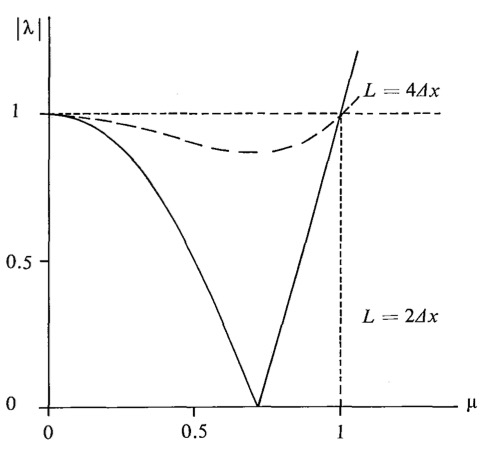
\includegraphics[keepaspectratio]{./pictest/pic12.jpg}}
\caption{}
\end{figure}

The Lax-Wendroff scheme has been fairly widely used in atmospheric
models, due to a recommendation by Richtmyer (1963), and its reasonably
good behaviour. It is second order accurate, explicit, not
unconditionally unstable, and since it is a two levels scheme there is
no computational mode. None of the schemes obtained by combining
centered space differencing with one of the seven time differencing
schemes studied in chapter \texttt{Chapter2} has all of these
advantages. The dissipation of the Lax-Wendroff scheme will not be
harmful if its total effect is negligible compared with the physical
dissipation, and it can also be useful for controlling the shortest
waves. If the physical dissipation is very small or non-existent, it is
better to use a neutral scheme.

One should point out here that we can change the time differencing
scheme intermittedly during an integration, so as to get the required
amount of a particular effect. For example, in the general circulation
model developed at the National Center for Atmospheric Research,
Boulder, Colo., the Lax-Wendroff scheme is used because of its damping
effect on the shortest waves. However, to keep the amount of damping
small, it is used only once in every hundred steps, the rest are made
using a neutral leapfrog scheme (Kasahara, 1969). On the other hand, in
the British operational model (e.g. Gadd, 1974b) the Lax-Wendroff scheme
is used every time step, with the authors of the model making no mention
of any excessive damping due to the scheme for the purposes of that
model

\subsection{\texorpdfstring{\textbf{Computational
dispersion}}{Computational dispersion}}\label{Section3.2}

As we have seen, the linear advection equation

{\[\frac{\partial u}{\partial t} + c\frac{\partial u}{\partial x} = 0\]\[c = const\]}

has a solution in the form of a single harmonic component

{\[u\left( x,t \right) = Re\left\lbrack U\left( t \right)e^{\text{ikx}} \right\rbrack\]}

provided that

{\[\frac{\text{dU}}{\text{dt}} + ikcU = 0\]}

In this oscillation equation \(kc\) is equal to the frequency \(\nu\),
and \(c = \frac{\nu}{k}\) is the phase speed of the waves. It is seen
that waves of all wave lengths are propagated with the same phase speed,
that is, the function \(u\left( x,t \right)\) is advected with no change
in shape at a constant velocity \emph{c} along the \emph{x} axis. There
is no dispersion.

Now consider the equation

{\[\frac{{\partial u}_{j}}{\partial t} + c\frac{u_{j + 1} - u_{j - 1}}{2\Delta x} = 0\]}

that is obtained by approximating the space derivative in \texttt{a2.1}
by a centered difference quotient. The equation \texttt{a2.4} is neither
a differential nor a difference equation, but a hybrid of these two. An
equation of this type can be called a differential-difference equation,
or a semi­ discrete equation. The finite difference equations obtained
when the time derivative in \texttt{a2.4} is approximated using a
consistent time differencing scheme will approach (\texttt{a2.4} as the
time step approaches zero. Thus, for small \(\Delta t\) \texttt{a2.4}
represents an approximation to these finite difference equations. Since
the time derivative has retained its differential form, any error in
\texttt{a2.4} is due to the space differencing.

For this reason, equations of this type are used to study the effect of
particular space difference approximations on the properties of the
numerical solution.

Recall that \texttt{a2.4} has a solution in the form of a single
harmonic component

{\[u_{j}\left( t \right) = Re\left\lbrack U\left( t \right)e^{\text{ikjx}} \right\rbrack\]}

provided that

{\[\frac{\text{dU}}{\text{dt}} + ik\left( \frac{\sin{k\Delta x}}{k\Delta x} \right)U = 0\]}

We have now written this so that it can conveniently be compared with
\texttt{a2.3} . Instead of the constant phase speed c, we see that waves
now propagate with the phase speed

{\[c^{*} = c\frac{\sin{k\Delta x}}{k\Delta x}\]}

This phase speed is a function of the wave number k. Thus, the finite
differencing in space causes a dispersion of the waves ; we shall call
this effect \emph{computational dispersion}. As \(k\Delta x\) increases
from zero, the phase speed \(c^{*}\) monotonically decreases from c, and
becomes zero for the shortest resolvable wave length \(2\Delta x\), when
\(k\Delta x = \pi\). Thus, all waves propagate at a speed that is less
than the true phase speed c, with this decelerating effect increasing as
the wave length decreases. The two-grid-interval wave is stationary.

The reason for the two-grid-interval wave being sta­tionary is obvious
when we look at the plot of that wave, shown in \texttt{figg:13}. For
this wave \(u_{j + 1} = u_{j - 1}\) at all grid points, and
\texttt{a2.4} gives a zero value for
\(\frac{{\partial u}_{j}}{\partial t}\)

We have encountered two effects here. Firstly, the advection speed is
less than the true advection speed. The consequence of this error is a
general retardation of the advection process. Secondly, the advection
speed changes with wave number; this false dispersion is particularly
serious for the shortest waves.

\begin{figure}
\centering
\pandocbounded{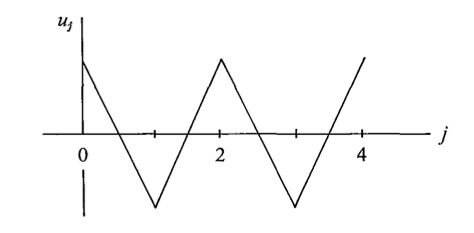
\includegraphics[keepaspectratio]{./pictest/pic13.jpg}}
\caption{}
\end{figure}

If the pattern that is being advected represents a super­position of
more than one wave, this false dispersion will result in a deformation
of that pattern. It is especially small-scale patterns in the
atmosphere, e.g. fronts, shear lines, etc., that represent a
superposition of many waves, including a significant proportion of the
shortest waves. For this reason, in numerical forecasting, such
patterns, if present in the initial fields, are fairly rapidly deformed,
until they aquire a form which is less sharp than in the beginning.
Since such small-scale features are of particular importance in weather
processes, the effect of computational dispersion deserves very careful
consideration.

We now turn our attention to the group velocity. In the case of the
linear equation \texttt{a2.1} we obtain for the group velocity \(c_{g}\)

{\[\tau_{c} = \frac{d\left( \text{kc} \right)}{\text{dk}} = c\]}

Thus, the group velocity is constant and equal to the phase speed \(c\).
With the differential-difference equation \texttt{a2.4} , however,
\texttt{a2.7} gives for the group velocity c*

{\[c_{g} = \frac{d\left( kc^{*} \right)}{\text{dt}} = c\cos{k\Delta x}\]}

Thus, as \(k\Delta x\), increases from zero, the group velocity
\(c_{g}\), decreases monotonically from \(c_{g}\), and becomes equal
\({- c}_{g}\) for the shortest resolvable wave length of
\(2k\Delta\text{x.}\)

These results are summarized in \texttt{figg:14}. For the exact
advection equation \texttt{a2.1} both individual waves and wave packets,
that is, places where superposition of waves results in a maximum
amplitude of a group of neighbouring wave numbers, propagate at the same
con­stant velocity \(c = c_{g}\). Introduction of the centered space
finite difference quotient in (2.4) both makes the phase speed and the
group velocity decrease as the wave number increases. The error is
particularly great for the shortest resolvable wave lengths; waves with
wave lengths less

\begin{figure}
\centering
\pandocbounded{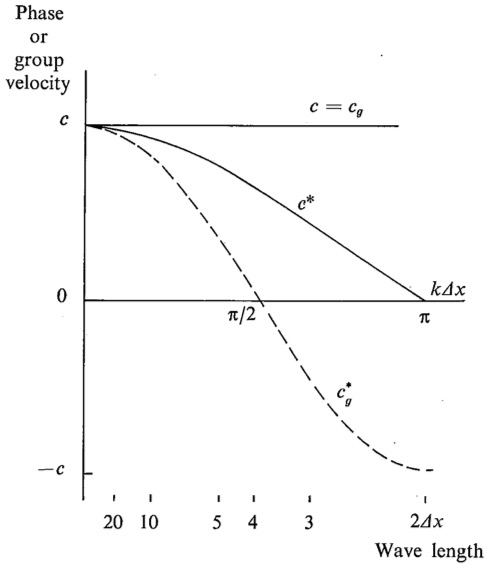
\includegraphics[keepaspectratio]{./pictest/pic14.jpg}}
\caption{}
\end{figure}

Than \(4\Delta x\) even have a negative group velocity. This means that
wave packets made up of these waves propa­gate in the direction opposite
to the advection velocity and opposite to the direction of propagation
of individual waves.

This situation can be illustrated by a simple example. Let us define Y
(x) as a function that is slowly varying in space; for example, it can
be a sine function of a large wavelength. Furthermore, we define

{\[u_{j} \equiv \left( - 1 \right)^{j}Y_{J}\]}

as shown in \texttt{figg:15}. Thus, the function ±Y(x) is the envelope
of the function \(u_{j}\). Suppose that we calculate the advection of
\(u_{j}\) using \texttt{a2.4} , then substituting \texttt{a2.10} into
\texttt{a2.4} we obtain

\[\frac{\partial Y}{\partial t} - c\frac{Y_{J + 1} - Y_{J - 1}}{2\Delta X} = 0\]

Thus, the advection of \(Y_{j}`is governed by the same equation
as the advection of :math:`u_{j}`except that the advection velocity
appears with an opposite sign ! Therefore, as the individual short waves
of the function :math:`u_{j}\) slowly propagate in the direction of the
positive x axis, the envelope \(\pm Y\left( x \right)\), which has a
long wave length, propagates rela­tively fast in the opposite direction.
When it is a sine function, so that it consists of a single harmonic, it
propagates with no change in shape. Because of (2.10), u\} must also be
advected with no change in shape ; from this we conclude that u\} also
consists of a single harmonic component. If, on the other hand, the
function \(Y\left( x \right)\) consisted of a number of harmonic
components, the shapes of both \(Y( x )\) and \(u_{j}\) would change
during the advection process, as a result of the computational
dispersion of these components.

It is possible to obtain an analytic solution of \texttt{a2.4} , which
can be used to analyze its behaviour for some given initial conditions
of interest. To this end it is convenient to define a non-dimensional
time variable

{\[\tau \equiv \frac{\text{ct}}{\Delta x}\]}

\begin{figure}
\centering
\pandocbounded{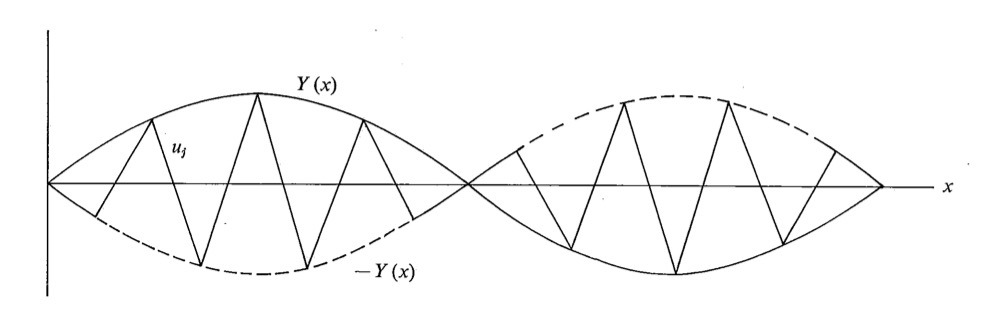
\includegraphics[keepaspectratio]{./pictest/pic15.jpg}}
\caption{}
\end{figure}

and, after dividing equation \texttt{a2.4} by \(\frac{c}{2\Delta x}\),
to write it in the form

{\[2\frac{d}{d\tau}u_{j}\left( \tau \right) = u_{j - 1}\left( \tau \right) - u_{j + 1}\left( \tau \right)\]}

This can be recognized as the recurrence formula of the Bessel function
of the first kind of order \(j,J_{j}\left( \tau \right)_{,}\) (e.g.
Courant and Hilbert, 1953, p. 488). In other words,

{\[u_{j}\left( \tau \right) = J_j\left( \tau \right)\]}

is a solution of \texttt{a2.12}. Several of these functions, of the
lowest order, are shown in \texttt{figg:16}. The figure illustrates more
of these functions than indicated, since, for any \(j\),

\[J_{- j} = \left( - 1 \right)^{j}J_{j}\]

Note, furthermore, that in \texttt{a2.12} the subscript \emph{j} can
take any integer value, since the location of the grid point for which
we choose \(J = 0\) is arbitrary. Thus, a solution that is more general
than \texttt{a2.13} is

\[u_{j}\left( \tau \right) = J_{j - p}\left( \tau \right)\]

\begin{figure}
\centering
\pandocbounded{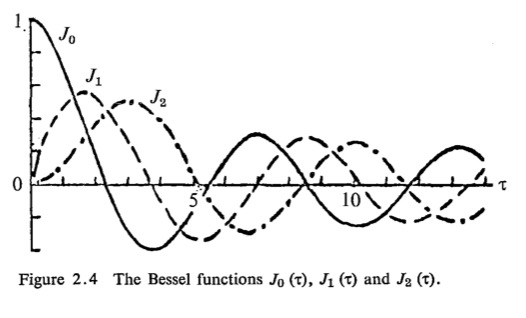
\includegraphics[keepaspectratio]{./pictest/pic16.jpg}}
\caption{}
\end{figure}

Where \(p\) is an arbitrary integer. Since we are solving a linear
equation, a still more general solution is a linear combination of all
these solutions, that is

{\[u_{j}\left( \tau \right) = \sum_{p = - \infty}^{\infty}{a_{p}J_{j - p}}\left( \tau \right)\]}

where \(a_{p}\) are arbitrary constants. Now, for \(\tau = 0\) all of
the functions \(J_{k}\) are equal to zero, except \(J_{0}\), for which
\(J_{0}\left( 0 \right) = 1\). Hence, substituting \(\tau = 0\) into
\texttt{a2.14} we obtain

{\[u_{j}\left( 0 \right) = a_{j}\]}

Therefore the constants in \texttt{a2.14} can be chosen so as to satisfy
arbitrary initial conditions \(u_{j} = u_{j}\left( 0 \right)\). Since it
can satisfy arbitrary initial conditions, \texttt{a2.14} is seen to
represent the general solution of \texttt{a2.12}, or \texttt{a2.4}.

It is instructive to look in some detail at the solution satisfying the
initial conditions

{\[\begin{aligned}
u_{j}\left( 0 \right) = \left\{ \begin{array}{cc}
1  &  for \quad j = 0\\
0  &  for \quad j \neq 0\\
\end{array} \right.
\end{aligned}\]}

the simplest solution of the form \texttt{a2.13}, for different values
of the non-dimensional time. At the initial moment the function u\}
consists of a single pulse-like disturbance, centered at the point
\(j = 0\), as shown in the upper diagram of \texttt{figg:17}. We note
that, because of \texttt{a2.12}, \(\frac{\text{du}_{j}}{\text{dt}}\) is
then equal to zero at all points except at \(j = - 1\) and \(j = 1\),
where it is equal to —1/2 and 1/2, respectively.

Thus, at the initial moment the disturbance propagates at the same rate
in the directions of both the positive and the negative x axis. Further
propagation of the dis­turbance according to \texttt{a2.13} can be
followed using \texttt{figg:8}, or, more accurately, using some tables
of Bessel functions. Solutions obtained in this way for \(\tau = 5\) and
\(\tau = 10\) are shown in the middle and lower diagrams of
\texttt{figg:17}, respectively.

\begin{figure}
\centering
\pandocbounded{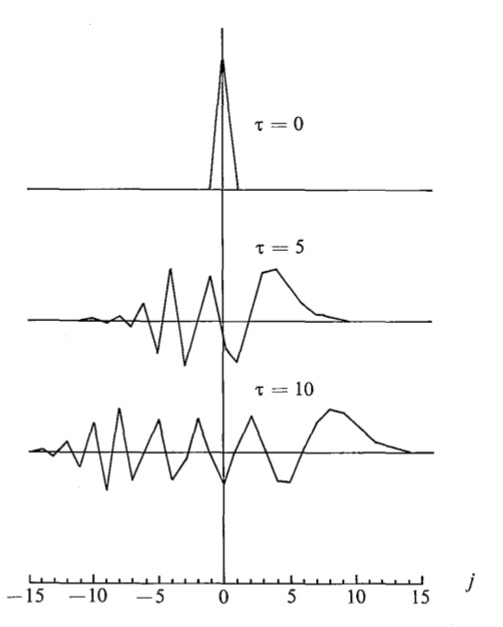
\includegraphics[keepaspectratio]{./pictest/pic17.jpg}}
\caption{}
\end{figure}

The three diagrams present an example of the computa­tional dispersion
of the second-order centered space differencing. We note that if we
expand a single pulse­like disturbance as a cosine Fourier integral

\(u\left( x \right) = \int_{0}^{\infty}{a\left( k \right)\cos\text{kxdk}}\),

\(a\left( k \right) = \frac{2}{\pi}u\left( x \right)\cos\text{kxdx}\),

and a(k) is calculated numerically using the grid point values only, we
obtain a constant value

\(a\left( k \right) = \frac{2}{\pi}\Delta x\)

Therefore, all the harmonic components have equal amplitude. By analogy
with the light spectrum, such a function is called white noise if it
does not appear for physical reasons. Its Fourier components are
advected with different phase speeds, as summarized in \texttt{figg:14},
bringing about a dispersion of the disturbance. With the non-dimensional
time chosen here we see from \texttt{a2.12} that the physical advection
velocity should keep the pulse located at the point \(j = \tau.\)
Because of the space difference approximation, however, all the phase
speeds are less than the physical advection velocity. The main
distur­bance, as seen in \texttt{figg:17}, is advected at a speed only
slightly less than the physical one ; obviously it mostly consists of
the longer wave components, which have an advection speed not much
different from the physical advection velocity. However, it is seen to
be diffusing away with time, which is again a result of the dispersion.
We also observe propagation of a group of short waves in the direction
opposite to that of the physical advection. Since the appearance of
these waves contradicts the physical properties of the advection
equation, such waves are called parasitic waves.

The solution of the differential-difference equation is, obviously,
quite unsatisfactory as an approximation to the true solution. However,
this example, with the initial disturbance located at one point only, is
completely unsuitable for a good solution by a difference
approxima­tion. This is exactly the reason why it provides an
in­structive illustration of the difficulties involved.

Analytic solutions for a more general case, when a centered difference
approximation is made to the time derivative also have been considered
by Egger (1971).

\subsection{\texorpdfstring{\textbf{Schemes with uncentered space
differencing}}{Schemes with uncentered space differencing}}\label{schemes-with-uncentered-space-differencing}

The space derivative in \texttt{a2.1} can also be approximated using
uncentered differencing. Still using values at two points for this
approximation it is attractive for physical reasons to have one of these
points as the central point and the second located on the side from
which the fluid is being advected toward the centre. Therefore we
approximate \texttt{a2.1} by

{\[\begin{aligned}
\frac{\partial u_j}{\partial t} + c\frac{u_{j} - u_{j - 1}}{\Delta x} &= 0, \quad \textrm{for}
\quad c > 0 \\
\end{aligned}\]\[\begin{aligned}
\frac{\partial u_j}{\partial t} + c\frac{u_{j+1} - u_{j}}{\Delta x} &= 0 \quad \textrm{for}
\quad c < 0 \\
\end{aligned}\]}

These equations are again differential-difference equa­tions. The first
equation in \texttt{a3.1} employs the backward and the second in
\texttt{a3.1} the for­ward difference quotient for the approximation to
the space derivative. However, in both cases the differences are
calculated on the side from which the advection velocity reaches the
centre; hence, these differences are called \emph{upstream differences}.
Calculated on the opposite side the differences would be called
downstream differ­ences.

Eqs. \texttt{a3.1} can be used to construct schemes for the advection
equation, by approximating the time derivative by one of the many
possible consistent methods. The resulting schemes will only be of the
first order of accuracy. However, they have a particular advantage over
centered schemes in space when applied to the advection of a disturbance
similar to the one considered in the preceding section. This is that,
with upstream differences, a dis­turbance cannot propagate in the
direction opposite to the physical advection. Thus, no parasitic waves
will contaminate the numerical solution.

If, specifically, a forward difference is used for the time derivative
in \texttt{a3.1}, we obtain, for \emph{c \textgreater{} 0},

{\[\frac{u_j^{n + 1} - u_j^{n}}{\Delta t}
+c \frac{u_j^{n} - u_{j - 1}^{n}}{\Delta x} = 0\]}

This is the scheme that was used for the examples of the introductory
chapter. It was found that this scheme was damping, with the amount of
damping depending on the wave length, with a maximum for the shortest
resolv­able wave length of \(2\Delta x\). The analytic solution of the
difference equation \texttt{a3.2} has been discussed by Wurtele (1961).

The advantage that is accomplished, at least in prin­ciple, by using
upstream differencing as compared with centered or downstream
differencing, can be illustrated by considering the \emph{domain of
influence} of a grid point in different schemes. We still consider the
case \emph{c \textgreater{} 0}.

\begin{figure}
\centering
\pandocbounded{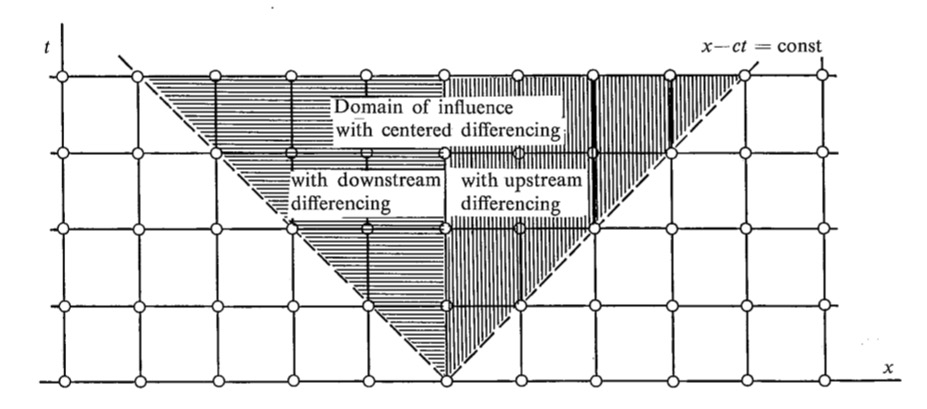
\includegraphics[keepaspectratio]{./pictest/pic31.jpg}}
\caption{}
\end{figure}

In the true solution, a grid point value can be said to propagate along
the characteristic \emph{x - ct} = const. \texttt{figg:31} shows a grid
point marked by a circle with the associated characteristic passing
through it. With upstream differencing as in \texttt{a3.2}, the value at
that grid point will influence the values at points within the domain
shaded by vertical lines. The figure also shows the domains of influence
with centered and downstream differencing. Of the three domains of
influence, that given by upstream differencing is clearly the best
approxi­mation to the characteristic line representing the domain of
influence in the true solution.

This discussion suggests constructing a scheme for \texttt{a2.1} by
tracing a characteristic back from the point
\(\left( j\Delta x,\left( n + 1 \right)\Delta t \right)\) to intersect
the previous time level \(\tau = n\Delta t\) and calculating the value
\(u^{*}\) at the point of inter­section by interpolation. We then set
\({u_{j}^{n + 1} = u}^{*}\). Choosing a linear interpolation procedure,
that employs values at two neighbouring points at the time
\(n\Delta t\), we obtain

\(u_{j}^{n + 1} = u_{j - 1}^{n} + \frac{u_{j}^{n} - u_{j - 1}^{n}}{\Delta x}\left( \Delta x - c\Delta t \right)\)

This can be identical to the scheme \texttt{a3.2}, with up­stream
differencing. If, on the other hand, a quadratic interpolation procedure
is chosen, using three neighbor­ing points, one obtains the Lax-Wendroff
scheme, as the reader can readily verify.

For further insight into the properties of schemes that can be obtained
from \texttt{a3.1} we consider the analytic solution of this
differential-difference equation. For small values of \(\Delta t\) this
will approximate the solution obtained from the difference schemes. As
before we introduce the non-dimensional time
\(\tau = \frac{\text{ct}}{\Delta x}\). Eq. \texttt{a3.1} can then be
written as

{\[\frac{d}{d t}u_{j}\left( \tau \right) + u_{j}\left( \tau \right) - u_{j - 1}\left( \tau \right) = 0\]}

A solution of this equation is the Poisson frequency function

{\[\begin{aligned}
u_j(\tau) = \left\{ \begin{array}{cc}
&\frac{e^{- \tau}\tau^{j - p}}{(j-p)!} \qquad &\textrm{for} \quad j \geq p \\
& 0  \qquad &\textrm{for} \quad j < p\\
\end{array} \right.
\end{aligned}\]}

as can easily be checked by substitution. Here \emph{p} is again an
arbitrary integer, that is, we have already taken into account the fact
that the location of the point \emph{j} = 0 is arbitrary.

\begin{figure}
\centering
\pandocbounded{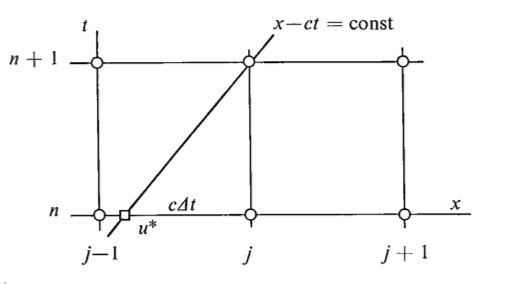
\includegraphics[keepaspectratio]{./pictest/pic32.jpg}}
\caption{}
\end{figure}

\begin{figure}
\centering
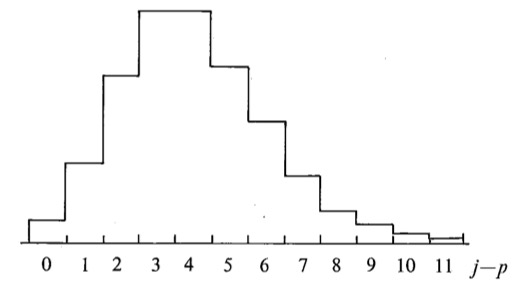
\includegraphics[width=0.8\linewidth,height=\textheight,keepaspectratio]{./pictest/pic33.jpg}
\caption{The Poisson frequency function \texttt{a3.4}, for the case
\(\tau = 4\).}
\end{figure}

An example of the Poisson frequency function is shown in
\texttt{figg:33}; the graph in the figure represents the shape of this
function for \(\tau = 4\). There is no need to include a vertical scale,
since the area enclosed by the graph of a frequency function has to be
equal to unity, so

{\[\sum_{j - p = 0}^{\infty}\frac{e^{- \tau}\tau^{j - p}}{\left( j - p \right)^{!}} = 1\]}

Thus, for \(\tau = 0\), when, as shown by \texttt{a3.4}, the histogram
consists of a single rectangle, its ordinate is equal to unity.

Consider now the change in shape of the histogram \texttt{a3.4} as the
non-dimensional time \(\tau\) increases from zero. The initial shape of
this histogram, that of a parallelogram having a base \(\Delta x\) and
erected at a single grid point, is, of course, equivalent to the shape
of the pulse-like disturbance \texttt{a2.16} used for the example of the
previous section. As τ increases beyond zero \texttt{a3.4} transforms
into a skewed bell-shaped histogram of the type as shown in the figure,
with its mean position on the \emph{x} axis

\[\sum_{j - p = 0}^{\infty}\left( j - p \right)\frac{e^{- \tau}\tau^{j - p}}{\left( j - p \right)^{!}} = \tau\]

moving at a constant speed. Thus, the mean position propagates with a
speed equal to the physical advection velocity. The maximum point of the
histogram, however, lags behind as is shown by the skewed shape of the
histo­gram. Physically unjustified negative values of \(u_{j}\), never
occur and no parasitic waves appear on the opposite side of zero from
the direction of the physical advection. Furthermore, as follows from
\texttt{a3.5}, the total amount of the advected quantity is exactly
conserved. However, the disturbance is damped out during the advection
process at quite a high rate.

As in Section \texttt{Section3.2} we can form a solution more general
than \texttt{a3.4}, as a linear combination of all possible solu­tions
\texttt{a3.4}, that is

{\[u_{j}\left( \tau \right) = \sum_{p = - \infty}^{j}a_{p}\frac{e^{- \tau}\tau^{j - p}}{\left( j - p \right)^{!}}\]}

where \(a_{p}\) are arbitrary constants. Substituting \(\tau = 0\) into
\texttt{a3.6} we obtain

{\[u_{j}\left( 0 \right) = a_{j}\]}

Thus, the constants \(a_{p}\) can again be chosen so as to satisfy
arbitrary initial conditions \(u_{j} = u_{j}(0)\), and so \texttt{a3.6}
represents the general solution of \texttt{a3.3}, or \texttt{a3.1}.
Considering the behaviour of the simple solution \texttt{a3.4}, and the
summation limits in \texttt{a3.6}, we see that in general the value
\(u_{j}\left( \tau \right)\) at a point \emph{j} can be considered as a
result of superposition of the effect of the initial values at that
point and of the initial values at all the points located
\emph{upstream} of it.

An example of the solutions \texttt{a2.14}, for centered differencing,
and \texttt{a3.6}, for upstream differencing, for an initial disturbance
of a somewhat larger space scale

\[\begin{aligned}
u_{j}(0) = \left\{ \begin{array}{cc}
1  &\textrm{for} \quad j = -1,0,1\\
0  &\textrm{for} \quad j \neq -1,0,1\\
\end{array} \right.
\end{aligned}\]

is shown in \texttt{figg:34}. If the grid distance is of the order of
300 km, and c is about 15 msec-1 we can see that 5 units of
non-dimensional time approximately corres­pond to the physical time of
one day. Thus, the damping effect of the upstream differencing is seen
to be quite severe. The figure also illustrates the properties of the
two methods described, but to a lesser extent than the examples with the
initial disturbance limited to a single grid point only. Thus we can
hardly claim that the use of upstream differencing instead of centered
second-order differencing has, generally speaking, improved the
solution.

\begin{figure}
\centering
\pandocbounded{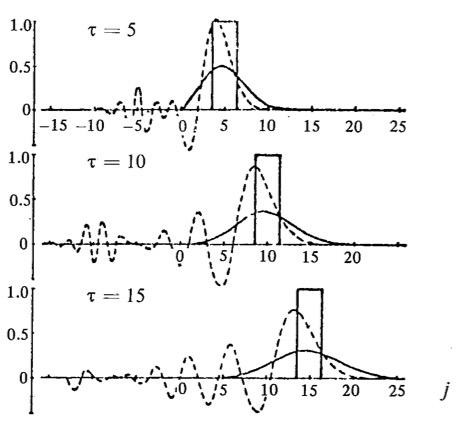
\includegraphics[keepaspectratio]{./pictest/pic34.jpg}}
\caption{}
\end{figure}

\subsection{\texorpdfstring{\textbf{Schemes with centered fourth-order
space
differencing}}{Schemes with centered fourth-order space differencing}}\label{schemes-with-centered-fourth-order-space-differencing}

Most of the difficulties that have been discussed in this chapter, in
particular the phase speed error and the computational dispersion, have
been due to the approxi­mations used for space differencing. Thus,
consideration should be given to other possibilities; one is to employ
approximations of a higher order of accuracy. We shall first construct
such an approximation.

When the approximate value \(u_{j}\) are expanded into Taylor series
about the central point, and substituted into the finite difference
quotient, we obtain

{\[\frac{u_{j + 1} - u_{j - 1}}{2\Delta x} = \frac{\partial u}{\partial x} +
\frac{1}{3!}\frac{\partial^3 u}{\partial x^3}( \Delta x )^{2} +
O\left\lbrack \left( \Delta x \right)^{4} \right\rbrack                \]}

Thus, this quotient is of the second order of accuracy. It is formed by
taking differences of values of \(u_{j}\) at points one grid distance
away from the central point. Similarly a quotient can be formed by
taking differences of values two grid distance away. We then obtain,
replacing \(\Delta x\) in \texttt{a4.1} by \(2\Delta x\),

{\[\frac{u_{j + 2} - u_{j - 2}}{4\Delta x} = \frac{\partial u}{\partial x} +
\frac{4}{3!}\frac{\partial^3 u}{\partial x^3}( \Delta x )^{2} +
O\left\lbrack \left( \Delta x \right)^{4} \right\rbrack \]}

This quotient is still second order accurate, but the coefficients are
larger. Other consistent approximations to
\(\frac{\partial u}{\partial x}`can be formed as linear
combinations of the quotients :eq:`a4.1\) and \texttt{a4.2}. The
combination for the second order terms in the truncation errors of
\texttt{a4.1} and \texttt{a4.2} cancel is particularly important. This
is

{\[\frac{4}{3}\frac{u_{j+1} - u_{j-1}}{2\Delta x} - \frac{1}{3}\frac{u_{j+2} - u_{j-2}}{4\Delta x} 
= \frac{\partial u}{\partial x} 
+ O\left\lbrack \left( \Delta x \right)^{4} \right\rbrack\]}

And represets a fourth-order accurate approximation to
\(\frac{\partial u}{\partial x}\).

We can also think of the approximation \texttt{a4.3} as repre­senting a
linear extrapolation of the quotients \texttt{a4.2} and \texttt{a4.1} so
as to simulate an approximation corresponding to differences taken
between points at a distance \emph{d} less than \(\Delta x\) away from
the centre. A simple calculation shows that the approximation
\texttt{a4.3} is obtained by extrapolation for the value
\(d = \frac{2\Delta x}{3}\). Of course, there is no reason to expect
that the accuracy of such an approximation should decrease monotonically
as \emph{d} decreases.

We now want to look at the effect on the phase speed of using the
approximation \texttt{a4.3} for the space derivative in the advection
equation. Replacing the space derivative in \texttt{a2.1} by
\texttt{a4.3} we obtain the differential-difference equation

{\[\frac{\partial u_{j}}{\partial t} + c\left( \frac{4}{3}\frac{u_{j + 1} - u_{j - 1}}{2\Delta x} - \frac{1}{3}\frac{u_{j + 2} - u_{j - 1}}{4\Delta x} \right) = 0\]}

As in Section \texttt{Section3.2}, we investigate the behavior of a
tentative solution in form of a harmonic component

\[u_j( t ) = Re\left\lbrack U\left( t \right)e^{ikj\Delta x} \right\rbrack\]

With second-order space differencing, we obtain the phase speed

\[c^{*} = c\frac{\sin{k \Delta x}}{k \Delta x}\]

Now, in the same way, with fourth-order differencing we find the phase
speed

{\[c^{**} = c\left( \frac{4}{3}\frac{\sin{k\Delta x}}{k \Delta x} 
- \frac{1}{3}\frac{\sin{2k\Delta x}}{2k\Delta x} \right)\]}

We shall compare these two results. For second order differencing, we
obtain by series expansion for small values of k

\[c^{*} = c\left( 1 - \frac{1}{3!}\left( k\Delta x \right)^{2} + \ldots \right)\]

On the other hand, with fourth order differencing we have

\[c^{**} = c\left( 1 - \frac{4}{5!}\left( k\Delta x \right)^{4} + \ldots \right)\]

Thus, even though the decelerating effect is still present, the phase
speed error has been much reduced for small values of \emph{k}.

These phase speeds are shown in \texttt{figg:41} as functions of
\(k\Delta x\), for all admissible values of \emph{k}. The figure
illus­trates the very significant increase in accuracy of the phase
speed for large-scale and medium-scale waves. However, as the wave
length approaches its minimum value of \(2\Delta x\) the increase in
phase speed obtained by fourth order differencing diminishes, until,
finally, the wave with wave length \(2\Delta x\) is again stationary.

\begin{figure}
\centering
\pandocbounded{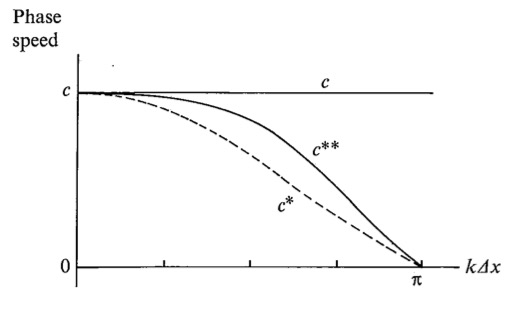
\includegraphics[keepaspectratio]{./pictest/pic41.jpg}}
\caption{}
\end{figure}

Moreover, for short waves the slope of the phase speed curve is greater
than with second order differencing, and, therefore, the computational
dispersion of these waves is greater. Thus, although a short wave-length
disturb­ance will now be advected at a somewhat greater speed its false
deformation, due to computational dispersion, will be faster.

Because of the decrease in the phase speed error of the longer waves,
the use of fourth order schemes for advec­tion has brought about
significant improvements in operational numerical forecasting in both
the U.S.A. and Japan, in barotropic and quasi-geostrophic baroclinic
models. With primitive equation models, now in use in all advanced
forecasting centres, fourth order advection schemes are not yet quite so
widespread. Still, it is gener­ally believed that fourth-order advection
schemes should be used in operational forecasting. However, the use of
advection schemes of a high-order of accuracy in general circulation
models may not be so important. The choice is between increasing the
accuracy of space differencing or spending an equivalent amount of extra
computation time in reducing the grid size of the model. A
straight­forward calculation (e.g. Thompson, 1961, p. 157) shows that
the first alternative should be advantageous.

The use of the additional grid points needed for higher order
differencing does create some side difficulties. In much the same way as
using more than two levels for time differencing resulted in the
appearance of computa­tional modes in time, so the use of additional
grid points for space differencing results in the appearance of
compu­tational modes in space. Furthermore, formulation of boundary
conditions becomes more complicated. Simply formulated boundary
conditions may be a source of serious problems.

For small scale disturbances, of a scale close to two grid intervals in
space, no finite difference method is really satisfactory. Additional
ways of constructing difference schemes for the advection equation are
discussed in the paper by Anderson and Fattahi (1974) where further
references are given. If it is felt that, in a particular situation, the
improvement of the advection of scales close to two grid intervals is
necessary, the obvious method is to find a way of making the computation
with a reduced grid size. As can be inferred from \texttt{figg:41},
halving the grid size with simple second-order differencing makes the
stationary two-grid-interval wave move at a speed of almost 2/3 of its
physical advection speed. But this, of course, is not easily attainable:
in two-dimensional problems, halving the grid size increases the
computational time requirements by a factor of four, and, with the usual
time difference schemes by an addi­tional factor of two in order to
maintain computational stability. Still, a steady increase in the
capabilities of commercially available computers enables constant
improvements of this kind, so that it is expected that in a few years
the resolution of atmospheric models may be such that advection errors
will not be a major problem. At present it is estimated that the
horizontal truncation errors in the advection terms are the largest
single source of errors in short range numerical forecasting, accounting
for almost 40 per cent of the total error (Robert, 1974).

Another way of improving the advection of small scale systems may be to
develop a computational method more in spirit of the Lagrangian system
of equations. As yet, such methods have not been very much explored in
meteorology.

\subsection{\texorpdfstring{\textbf{The two-dimensional advection
equation}}{The two-dimensional advection equation}}\label{the-two-dimensional-advection-equation}

We now consider the two-dimensional linear advection equation

{\[\frac{\partial u}{\partial t} + c_{x}\frac{\partial u}{\partial x}+ c_y\frac{\partial u}{\partial y} = 0
\qquad c_x,\quad c_y = cost\]}

where \(u = u\left( x,y,t \right)`is a function of two space
variables, and :math:`c_{x},c_{y}\) are the components of the advection
velocity. Thus, the advection speed is given by

{\[c = \sqrt{c_{x}^{2} + c_{y}^{2}}\]}

We shall test the stability of schemes for the numerical solution of
\texttt{a5.1} by the procedure of Section \texttt{Section3.1}. Thus,
space derivatives are approximated by standard second-order difference
quotients, giving

{\[\frac{\partial}{\partial t}u_{i,j} = - c_{x}\frac{u_{i + 1,j} - u_{i - 1,j}}{2\Delta x} - c_{y}\frac{u_{i,j + 1} - u_{i,j - 1}}{2\Delta y}\]}

Here, as is usual for two-dimensional problems, we have changed the
choice of subscript denoting the grid points along \emph{x} axis, so
that the coordinates of the grid points are now \(x = i\Delta x\),
\(y = i\Delta y\), and approximate values
\(u\left( i\Delta x,j\Delta y \right)\) are denoted by \(u_{i,j}\). As a
tentative solution of \texttt{a5.3} we substitute

{\[u_{i,j} = Re\left\lbrack U\left( t \right)e^{i( kx + ly \)} \right\rbrack\]}

giving the oscillation equation

{\[\frac{d U}{d t} = i\left( - \frac{c_{x}}{\Delta x}\sin{k\Delta x} -\frac{c_{y}}{\Delta y}\sin{l\Delta y} \right)U\]}

If the leapfrog scheme is used for the time derivative, we obtain as the
stability criterion

{\[\left| \left( \frac{c_x}{\Delta x}\sin{k\Delta x} +
 \frac{c_y}{\Delta y}\sin{l\Delta y} \right)\Delta t \right| \leq 1\]}

This has to be satisfied for all admissible values of the wave numbers
\emph{k}, \emph{l}.

For simplicity, we shall consider only the cases where
\(\Delta x = \Delta y\) we denote this grid size by \(d^{*}\). In the
wave number plane, that is, a diagram with co-ordinates \emph{k, l}, the
admissible wave numbers are contained within the square region shown in
\texttt{figg:51}. Inside that region the maximum value of the left-hand
side of \texttt{a5.6} is obtained at the centre of the square, marked by
a circle. The wave represented by that point has wave lengths \(4d^*\)
in both the \emph{x} and \emph{y} directions so that
\(sink{\Delta x} = \sin{l\Delta y} = 1\).

\begin{figure}
\centering
\pandocbounded{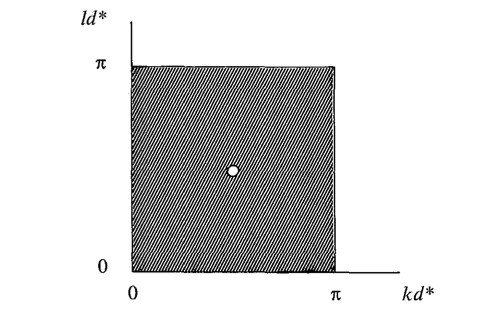
\includegraphics[keepaspectratio]{./pictest/pic51.jpg}}
\caption{}
\end{figure}

For a given value of the advection speed the left-hand side of
\texttt{a5.6} has a maximum value at this point if the advection
velocity makes an angle of \(\frac{\pi}{4}\) with the axis, in this case
\(c_{x} = c_{y} = \frac{\sqrt{2}}{2}c\). Thus we obtain the stability
criterion

{\[\sqrt{2}c\frac{\Delta t}{\Delta x} \leq 1\]}

Therefore, in the two-dimensional case we have to choose a time step
that is \(\sqrt{2}\) times less than that permitted in the
one-dimensional case. We note that the minimum stability is associated
with wave lengths in both the \emph{x} and \emph{y} directions twice as
long as the shortest resolvable wave length of \({2d}^{*}\), exactly as
in the one-dimensional case. The two-dimensional wave number of this
wave

\[\sqrt{k^{2} + l^{2}}\]

is, however, greater by a factor of \(\sqrt{2}\) than wave numbers along
the axes, and its wave length is therefore shorter by the same factor.
This applies to all waves with \emph{k} = \emph{l}.

\subsection{\texorpdfstring{\textbf{Aliasing error and nonlinear
instability}}{Aliasing error and nonlinear instability}}\label{aliasing-error-and-nonlinear-instability}

Another generalization of the simple one-dimensional linear advection
equation is to consider the nonlinear advection equation

{\[\frac{\partial u}{\partial t} + u\frac{\partial u}{\partial x} = 0\]}

We have returned to dimension, so that \emph{u} = \emph{u} (\emph{x},
\emph{t}).

Shuman (1974) calls \texttt{a6.1} the \emph{shock equation}. Its general
solution (e.g. Platzman, 1964) is

\[u = f\left( x - ut \right)\]

as can readily be verified. Here \emph{f} is an arbitrary function.

Here we consider only the effect of the multiplication in \texttt{a6.1}.
When performed in finite differences, it results in an error related to
the inability of the discrete grid to resolve wave lengths shorter than
\(2\Delta x\), that is, wave numbers greater than
\(k_{max} = \frac{\pi}{\Delta x}\). Thus, consider a function
\(u\left( x \right)\) which can be represented by values at grid points,
for example

{\[u = \sin{kx}\]}

where \({k < k}_{max}\) . However, substituting \texttt{a6.2} into the
nonlinear term of \texttt{a6.1} gives

\[u\frac{\partial u}{\partial x} = k\sin{kx}\cos{kx} = \frac{1}{2}k\sin{2kx}\]

Hence, if the wave number in \texttt{a6.2} is in the interval
\(\frac{1}{2}k_{max} < k \leq k_{max}\), the nonlinear term will give a
wave number that is beyond the range that can be resolved by the grid.
It cannot, therefore, be properly reproduced in a finite difference
calculation.

To gain some insight into what happens in such a situation, consider a
wave for which \(k > K_{max}\). For example, let
\(L_{t} = \frac{4\Delta x}{3}\). A wave of that wave length is shown by
the full line in \texttt{figg:61}. Knowing only the values at grid
points we will not be able to distinguish this wave from the one shown
by the dashed line. Thus, with the convention adopted earlier which
assumes that the longest waves are present, we will make an error. This
is called \emph{aliasing error}.

\begin{figure}
\centering
\pandocbounded{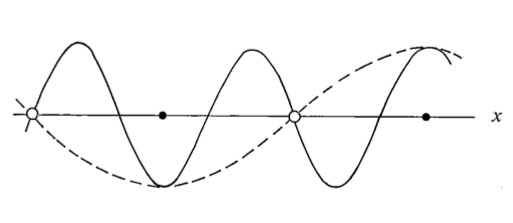
\includegraphics[keepaspectratio]{./pictest/pic61.jpg}}
\caption{}
\end{figure}

In a more general case, suppose that the function u consists of a number
of harmonic components

\[u = \sum_{n}^{}u_{n}\]

The nonlinear term will then contain products of harmo­nics of different
wave lengths, such as

\[\sin{k_1}x\sin{k_2}x\]

However,

\[\sin{k_1 x}\sin{k_2 x} = \frac{1}{2}
\left\lbrack \cos{( k_{1} - k_{2} )x - \cos{( k_{1} + k_{2} )x}} \right\rbrack\]

Thus, even if a finite difference calculation is started with waves
which all have \(k \leq k_{max}\), very soon through this process of
nonlinear interaction waves will be formed with \(k > k_{max}\) , and a
misrepresentation of waves will occur.

In general we can write

\[\sin{kx} = \sin{\left[ 2 k_{max} - ( 2 k_{max} - k ) \right] x}\]

Substituting here \(k_{max} = \frac{\pi}{\Delta x}\) and using the
formula for the sine of a difference, we obtain

\[\sin{kx} = \sin{\frac{2\pi}{\Delta x}x}\cos{\left( \frac{2\pi}{\Delta x} 
- k \right)}x - \cos{\frac{2\pi}{\Delta x}x}\sin{\left( \frac{2\pi}{\Delta x} - k \right)}x\]

However, at the grid points \(x = j\Delta x\) and

\[\sin\frac{2\pi}{\Delta x}j\Delta x = 0, \qquad \cos{\frac{2\pi}{\Delta x}j\Delta x = 1}\]

Therefore, we find

{\[\sin{k j \Delta x} = -\sin{\left( 2k_{max} - k \right)j\Delta x}\]}

In this way, we see that, knowing only the grid point values, we cannot
distinguish the wave numbers \(k\) from \(2k_{max} - k\) . Thus, if
\(k > k_{max}\), using the convention mentioned earlier, we can say that
the wave number k is misrepresented as the wave number

{\[k^{*} = 2k_{max} - k\]}

Hence, as shown in \texttt{figg:62}, the resulting wave has a wave
number \(k^{*}\) which is less than \(k_{max}\) by an amount equal to
that by which \(- k\) was greater than \( k_{max}\). W e can think of
the wave number \emph{k} * as being an image obtained by the reflection
of \emph{k} across the value \(k_{max}\) into the admissible range of
wave numbers.

\begin{figure}
\centering
\pandocbounded{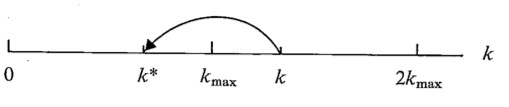
\includegraphics[keepaspectratio]{./pictest/pic62.jpg}}
\caption{}
\end{figure}

As an example consider the case \emph{L} = 4delta x /3, illustrated in
\texttt{figg:61}. Then \(k = 3\pi/2\Delta x\), and (6.4) gives
\(k^{*} = \frac{\pi}{2\Delta x}\) as the wave number "seen" by the
finite differ­ence grid. This, of course, is the same wave, of wave
length \(2\Delta x\), as the one found graphically and shown by the
dashed line.

Now consider the consequences of aliasing errors in a numerical
integration. An atmospheric variable, as a function of space
co-ordinates, can be thought of as consisting of a series of harmonic
components. It is useful to consider the "energy" of these components,
that is, their contribution to the mean square value of the variable
considered as a function of wave number.

This is the \emph{spectrum} of the "energy". For example, if the
variables are velocity components, this function is the kinetic
\emph{energy spectrum}. This spectrum describes the relative importance
of features of different scales in the field of the variable. Now,
experience shows that the spectrum of atmospheric variables does not
change much with time. On synoptic maps we do not have situations where
small scale features are dominant on one day, and absent on the next.
Accordingly, spectra of atmospheric variables also do not change much in
their general shape. The energy of a particular component can, of
course, change, but the characteristic shape of the spec­trum as a whole
is fairly constant. For example, a zonal spectrum of the eastward
velocity component in middle latitudes typically has a maximum for wave
numbers 4 to 7, that is, 4 to 7 wave lengths along a latitude circle,
with the energy tapering off rather rapidly as the wave number increases
beyond about 10. Thus, there is very little energy in wave numbers of
the order of the maximum wave numbers that can be resolved by finite
difference grids used in atmospheric models.

In a finite difference integration, in addition to these relatively
small physical changes, the shape of a spectrum is subject to changes
due to aliasing errors. If we have a spectrum of the shape just
described, and consider the representation of various combinations
\(k_1+k_2\) that are greater than \(k_{max}\), we see that most of the
energy of such combinations will belong to components with wave numbers
not much greater than \(k_{max}\) . Thus, due to aliasing errors a
spurious energy inflow is expected at wave numbers that are not much
less than \(k_{max}\), and, in time, the energy of these components can
be expected to grow beyond physically acceptable limits. Experience
shows that, if no precautionary measures are taken, this can indeed
happen, and even cause a catastrophic end to the integration. The
phenomenon is due to the nonlinear terms of the equations, and,
therefore, is called the \emph{nonlinear instability}. Nonlinear
instability was first en­countered by Norman Phillips (1956) in his
famous work that laid the foundation for the numerical modelling of the
atmospheric general circulation. Starting from an atmo­sphere at rest,
he integrated the vorticity equation for a simulated time of the order
of 30 days. The calculation then came to an end due to an explosive
increase in the total energy of the system, associated with an
appearance of elongated shapes in the vorticity field. Phillips
initially believed that the breakdown was due to excessive trunca­tion
errors, and he later repeated the experiment using space and time steps
both reduced to about half of their previous values. This must have
greatly reduced the trun­cation errors, but the catastrophic increase in
total energy still happened at about the same time.

In a later paper Phillips (1959) gave the interpretation of nonlinear
instability similar to what has been presented here, but for the
nondivergentvorticity equation. For a test of this explanation Phillips
again repeated his experiment, but after every two hours of simulated
time he performed a harmonic analysis of the vorticity fields, and
eliminated all components with \(k > \frac{1}{2}k_{max}\). If there are
no components with \(k > \frac{1}{2}k_{max}\) the advection term cannot
produce waves with \(k > k_{max}\) . We expect that it will be some time
before the amplitudes of the eliminated waves are built up again to an
appreciable extent. This filtering procedure eliminated the appear­ance
of the spurious increase in energy, thereby confirm­ing this explanation
of the instability.

\subsection{\texorpdfstring{\textbf{Suppression and prevention of
nonlinear
instability}}{Suppression and prevention of nonlinear instability}}\label{suppression-and-prevention-of-nonlinear-instability}

If an integration is to be performed for an extended period of time, it
is necessary to suppress or prevent nonlinear instability. For short
range integrations it is not necessary to do this, though such a
procedure might still have a beneficial effect on the model.

It has been pointed out by Orszag (1971) that to eliminate aliasing
errors it is not necessary to filter the top half of the admissible wave
numbers. It is sufficient to eliminate the top one-third, because, if
waves with \(k > \frac{2}{3}k_{max}\) are filtered out, all the aliases
satisfy \(k > \frac{2}{3}k_{max}\) and will thus be eliminated.

If, however, we consider that such a suppression of the shortest waves
is a satisfactory method of dealing with the problem, it would be
simpler to use a differencing scheme that has a built-in damping of the
shortest waves. This idea is due to Richtmyer (1963), who sug­gested use
of the Lax-Wendroff scheme for this purpose. It was found by experience
that such a practice does suppress the nonlinear instability, and that
to do this it is sufficient to use an intermittent Lax-Wendroff step at
quite long intervals (Kasahara, 1969). Kreiss and Oliger (1973), on the
other hand, recommend adding a dissipative term to a scheme which is not
dissipative, so that the amount of dissipation can be controlled in a
more practical way.

Another way of avoiding nonlinear instability is to use a Lagrangian
formulation of the advection terms instead of a Eulerian formulation. We
calculate the position of the parcel that should be advected to the grid
point considered in step \(\Delta t\). A value of the dependent variable
can be found corresponding to that position by interpola­tion in space.
The change due to advection is set equal to the difference between the
value obtained by interpola­tion and that at the grid point. In some
cases, these sche­mes turn out to be identical to schemes obtained using
the Eulerian formulation, but other schemes can also be obtained. A
procedure of this type was first used by Leith (1965); an example of its
use more recently is given in the paper by \emph{Krishnamurti et al}.
(1973).

A conceptually elegant approach for dealing with the nonlinear
instability problem has been suggested and developed by Arakawa (1966,
1972). His idea is that it is better, if possible, to use schemes for
the advection terms that are not only free of the nonlinear
computa­tional instability but also free of the spurious inflow of
energy to these short waves, instead of artificially suppress­ing their
amplitudes. The amplitudes of the shortest waves in atmospheric models
are small initially, and they will remain small if a false generation of
these short waves is avoided. Arakawa has shown that it is possible to
construct such schemes, and that they are obtained when care is taken to
conserve in the finite difference form some integral properties of the
original differential equa­tions.

When the Arakawa conservation schemes are used there is no need for an
artificial dissipation in the advec­tion process. This enables the
statistical properties of the schemes to be maintained under advection,
a feature especially useful in general circulation studies.

It has sometimes been argued that, because the phase error of the short
waves is very large, they should be eliminated before they erroneously
affect the longer waves through nonlinear interactions.. This argument
does not take account of several factors. If the phase speeds of the
short waves are wrong, the situation will not necessar­ily improve if
their amplitudes are also made wrong. They may still be performing a
useful function of a statistical nature. Also damping or elimination of
the shortest waves will also remove some energy from the longer waves
that we are interested in. If we wish to dissipate energy, it is
obviously better to do so for physical and not for computational
reasons.

We shall introduce the procedure of Arakawa by considering the vorticity
equation

{\[\frac{\partial\zeta}{\partial t} + \textbf{v} \cdot\nabla\zeta = 0,\qquad \zeta = \nabla^{2}\Psi\]}

where the velocity \(\textbf{v}\) is assumed to be nondivergent, that is

{\[\textbf{v} = \textbf{k} \times \nabla\Psi\]}

Substituting this into \texttt{a7.1} we obtain

{\[\frac{\partial}{\partial t}\nabla^{2}\Psi = J\left( \nabla^2\Psi, \Psi \right)\]}

This equation gives the local change in vorticity as a result of
advection by a two-dimensional nondivergent velocity. It is also a
nonlinear advection equation. However, in contrast with the
one-dimensional equation \texttt{a6.1}, \texttt{a7.3} gives a good
approximate description of large scale atmospheric processes. Thus, for
more than a decade it has been used as a basic prognostic equation for
the numerical weather prediction, eventually supple­mented by some
additional terms of a smaller order of magnitude.

To illustrate the Arakawa procedure for the vorticity equation (7.3), we
need some knowledge of its integral properties in wave number space. We
want to study the energy exchanges between different harmonics that are
permitted by that equation.

Consider first the kinetic energy spectrum when the velocity is
two-dimensional and nondivergent, so that it can be given by (7.2). We
can almost always assume that in the region considered A, the stream
function can be expressed as a series of orthogonal functions (e.g.
CourantandHilbert, 1953, p.369)

{\[\Psi = \sum_{n}^{}\Psi_{n}\]}

where the functions \(\Psi_n\) are eigenfunctions of the Helmholtz
equation

{\[\nabla^{2}\Psi_{n} + \lambda_{n}^{2}\Psi_{n} = 0\]}

The parameters \(\lambda_{n} \) are known as the \emph{generalized wave
numbers} of the components \(\Psi_{n}\)

As an example, let \emph{A} be a rectangular region with sides
\(L_x, L_y\). For boundary conditions assume that the stream function is
periodic in x with period \(L_{x}\) and is zero along the lower and
upper boundary. Then we can write the stream function

{\[\Psi = \sum_{n_1, n_2} \left( \alpha_{n_1, n_2}\cos{\frac{2\pi n_1}{L_x}x}+
 b_{n_1, n_2}\sin{\frac{2\pi n_1}{L_x}x} \right)\sin{ \frac{\pi n_2}{L_y} y}\]}

Differentiating this we obtain

\[\nabla^2\Psi_n = - \left\lbrack \left( \frac{2\pi n_1}{L_x} \right)^{2} +
\left( \frac{\pi n_2}{L_y}  \right)^{2} \right\rbrack\Psi_{n}\]

that is,

\[\lambda_n^2 = \left( \frac{2\pi n_1}{L_x} \right)^{2} + \left( \frac{\pi n_2}{L_y} \right)^{2}\]

If the region \emph{A} had different geometry, another set of orthogonal
functions would satisfy \texttt{a7.5} and the bound­ary conditions, and
could be used for the expansion \texttt{a7.4}. These functions will be
solutions of the Helmholtz equation \texttt{a7.5}.

Define the average of a variable a by

\[\overline{\alpha} \equiv \frac{1}{A}\int_A \alpha d A\]

We are interested in the average value of the kinetic energy per unit
mass

{\[\overline{K} = \frac{1}{2}\overline{( u^{2} + \nu^{2} ) } = \frac{1}{2}\overline{\nabla\Psi\cdot\nabla\Psi}\]}

Substituting \texttt{a7.4}, and assuming that this series can be
differentiated and integrated term by term, we obtain

\[\overline{K} = \frac{1}{2}\overline{ \nabla \sum_n\Psi_n\cdot\nabla\sum_m \Psi_m } 
= \frac{1}{2}\overline{  \sum_n\nabla\Psi_n\cdot\sum_m \nabla\Psi_m }  
= \frac{1}{2}\sum_m\sum_n \overline{ \nabla\Psi_m \nabla\Psi_n }\]

We note that

\[\nabla\Psi_m \nabla\Psi_n =\nabla \cdot \left( \Psi_m\nabla\Psi_n \right) - \Psi_m\nabla^2\Psi_n\]

Assume that no mass transport occurs through the bound­aries of A, that
is,

\[\overline{\nabla\cdot\left( \Psi_{m}\nabla\Psi_{n} \right)} = 0\]

Using \texttt{a7.5}, we then obtain

\[\overline{K} = -\frac{1}{2}\sum_m\sum_n \overline{ \Psi_m \nabla^2\Psi_n }
= -\frac{1}{2}\sum_m\sum_n \lambda_n^2\overline{ \Psi_m \Psi_n }\]

Since the functions \(\Psi_{n}\) are orthogonal, that is,

\[\overline{ \Psi_m \Psi_n } = 0 \qquad for m \neq n\]

the double sum reduces to a sum over only a single subscript, namely,

\[\overline{K} = \frac{1}{2}\sum_{n}\lambda_{n}^{2}\overline{\Psi_n^2}\]

We have therefore expressed the average kinetic energy in the region A
\emph{as a sum of contributions of different harmonics}

{\[\overline{K} = \frac{1}{2}\sum_{n}K_n\]}

Where

{\[K_{n} \equiv \frac{1}{2}\lambda_{n}^{2}\overline{\Psi_n^2}\]}

The contributions \(K_{n}\), considered as a function of n, represent
the kinetic energy spectrum. As seen from \texttt{a7.9}, they are never
negative. When the stream func­tion \(\Psi\) is known, the functions
\(\Psi_{n}\) can be computed by standard series expansion methods. In
fact, we calculate the coefficients of these components; in
\texttt{a7.4}, these coefficients have been absorbed into the functions
Since the values of \(\lambda_{n}\) are already known, for commonly used
geometries, we can calculate the kinetic energy spectra using
\texttt{a7.9}. Such a calculation, as well as the calculation of the
spectra of other variables, has been used for numerous studies of the
behavior and structure of both the observed and numerically simulated
fields of atmospheric variables.

The mean square vorticity

\[\overline{\zeta^2} = \overline{(\nabla^{2}\Psi^{2} )^2}\]

can be expressed as a sum of contributions of different harmonics in a
similar way. Substituting \texttt{a7.4}, using \texttt{a7.5}, and the
orthogonality of the functions \(\Psi_{n}\), we obtain

{\[\overline{\zeta^2} = \sum_{n}\lambda^{4}\overline{\Psi_n^2}\]}

Substituting the expression \texttt{a7.9} for the kinetic energy of a
component \(\Psi_{n}\); we find for the average value of the enstrophy
half the vorticity squared,

{\[\frac{1}{2}\overline{\zeta^{2}} = \sum_{n}\lambda_n^2 K_{n}\]}

Comparing this with \texttt{a7.8} we see that the average wave number is
related to average values of enstrophy and kinetic energy. Define the
average wave number as

{\[\lambda \equiv \sqrt{ \frac{\sum_n\lambda_n^2 K_n} {\sum_n K_n} }\]}

Substituting (7.11) and (7.8) we find

{\[\lambda = \sqrt{ \frac{\overline{\zeta_n^2} }{\overline{K}}  }\]}

Thus, when the velocity is two-dimensional and nondiver­gent, the
average wave number is determined by the ratio of the average values of
enstrophy and kinetic energy.

We originally wished to study the time dependence of the energy of
spectral components permitted by the vorticity equation \texttt{a7.3}.
It will suffice to look at the time dependence of \texttt{a7.13}. Then
\texttt{a7.3} gives

{\[\frac{\partial}{\partial t} \frac{1}{2} \overline{\zeta^2} =
\overline{\zeta \frac{\partial}{\partial t} \zeta } =
\overline{\zeta J(\zeta,\Psi)}\]}

Again assuming no mass transport through the bound­aries of A, we find

{\[\begin{aligned}
\frac{\partial}{\partial t} \overline{K} =
\frac{\partial}{\partial t} \frac{1}{2} \overline{(\nabla\Psi)^2} =
\overline{\nabla\Psi \cdot \frac{\partial}{\partial t}\nabla\Psi} =\\
-\overline{\Psi\frac{\partial}{\partial t} \nabla^2\Psi} =
-\overline{\Psi J(\zeta,\Psi)}
\end{aligned}\]}

However, for any two scalar quantities \emph{p,q} we have

\[J(p,q) = \textbf{k}\cdot\nabla \times \left( p\nabla q \right) = - \textbf{k}\nabla \times \left( p\nabla q \right)\]

Using Stokes\textquotesingle{} theorem, we see that

{\[\overline{J\left( p,q \right)} = 0\]}

if either \emph{p} or \emph{q} is constant along the boundary of
\emph{A}. Under the same conditions, we have

{\[\overline{p J\left( p,q \right)} = 0, \qquad \overline{q J\left( p,q \right)} = 0\]}

Therefore, if we assume that \(\Psi\) is constant along the boundary of
\emph{A}, \texttt{a7.14} and \texttt{a7.15} give

{\[\frac{1}{2}\overline{\zeta^{2}} =  const, \quad \text{and} \quad \overline{K} = const.\]}

In this way, we find that \emph{the average wave number does not change
with time} with two-dimensional nondivergent flow. In other words,
\emph{a systematic energy cascade toward higher wave numbers is not
possible}. Furthermore, since to obtain the enstrophy the contributions
\(K_{n}\) are multiplied by the wave number squared, \emph{the fraction
of the energy that can flow to high wave numbers is clearly limited, and
the higher the wave number, the more it is limited} (Fjortoft, 1953).

As pointed out by Charney (1966) this situation can be illustrated by a
simple mechanical analogy. The foregoing relations show that

\[\overline{K}\lambda^{2} = \sum_{n}K_{n}\lambda_{n}^{2} = \text{const}\]

On the left hand side here each of the two factors is constant, as the
first one is equal to the average energy. Thus, as shown in
\texttt{figg:71}, we can imagine a semi-infi­nite weightless rod on
which a weight \( \overline{k}\) is suspended at a distance
\(\lambda^{2}\) to the left of the point at which the rod itself is
suspended, and weights \(k_{1}k_{2}\ldots.. \) are sus­pended at
distances \(\lambda_{1}^{2}\lambda_{2}^{2}\ldots..\) right of that
point. The rod, as defined, would be in mechanical equilibrium. Its left
side, moreover, cannot change, while on the right hand side an
interchange of mass between weights is per­mitted, but only so as not to
disturb the equilibrium, that is, the total moment of forces. Thus, at
least three components must always take part in an energy transfer. In
particular very little energy can be expected to accu­mulate at the
highest wave numbers.

\begin{figure}
\centering
\pandocbounded{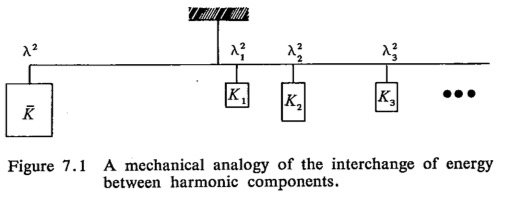
\includegraphics[keepaspectratio]{./pictest/pic71.jpg}}
\caption{}
\end{figure}

We now return to the numerical solution of \texttt{a7.3} and the
associated nonlinear instability problem. Obviously, if a finite
difference scheme could be constructed so as to conserve the average
values of enstrophy and the kinetic energy, the average wave number
would not change, and, therefore, a systematic transport of energy
toward the highest wave numbers would not be possible. Arakawa has
pointed this out, and showed that finite difference approximations can
be constructed that, indeed, maintain the properties \texttt{a7.17} of
the analytic Jacobian. Therefore, average enstrophy and kinetic energy
are conserved within the advection terms, and so is the average wave
number. Nonlinear instability is therefore prevented. His
approximations, in addition, maintain the property \texttt{a7.16}, and
thus also conserve the average vorticity. Thus the gross characteristics
of the frequency distribution of the vorticity field are also conserved.
The true non-divergent vorticity equation conserves all moments of the
frequency distribution of the vorticity since the area and the vorticity
of individual fluid parcels are both conserved. Maintaining properties
\texttt{a7.16} and \texttt{a7.17} in a finite difference calculation
will guarantee the conser­vation of the first two moments of this
distribution.

We illustrate Arakawa\textquotesingle s method by considering how to
satisfy \texttt{a7.17}. In our finite difference calculation it takes
the form

{\[\overline{\zeta_{ij}J_{ij}(\zeta,\Psi)} = \frac{1}{N}\sum_{i,j}\zeta_{ij}J_{ij}(\zeta,\Psi) = 0\]}

where \(J_{ij}\) denotes a finite difference approximation to the
Jacobian, and \(N\) the total number of grid points.

There are many ways of constructing finite difference approximations to
the Jacobian. We can use any of the three equivalent analytic
expressions

{\[\begin{aligned}
J(p,q) = \frac{\partial p}{\partial x}\frac{\partial q}{\partial y} -
\frac{\partial p}{\partial y}\frac{\partial q}{\partial x} =\\
\frac{\partial }{\partial y}q\frac{\partial p}{\partial x} -
\frac{\partial }{\partial x}q\frac{\partial q}{\partial x} =\\
\frac{\partial }{\partial x}p\frac{\partial q}{\partial y} -
\frac{\partial }{\partial y}p\frac{\partial q}{\partial x}
\end{aligned}\]}

We shall consider only approximations of the second order of accuracy.
With the simplest centered space differencing, we require values of
\(p\), \(q\) from a box of nine adjacent grid points to evaluate (7.20),
as shown in \texttt{figg:72}. Write \emph{d} for the grid size, and
\(p_{k}\), \(q_{k}\) for the values of \(p}\), \(q\) at the point
denoted by \(k\). We then obtain the following approximations to the
expressions \texttt{a7.2}

\begin{figure}
\centering
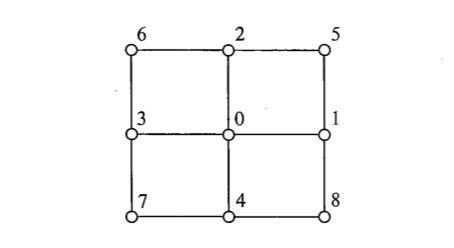
\includegraphics[width=0.8\linewidth,height=\textheight,keepaspectratio]{./pictest/pic72.jpg}
\caption{Stencil used to define approximations to Jacobian.}
\end{figure}

{\[J^{++}(p,q) = \frac{1}{4d^2} \left[ (p_1 - p_3)(q_2 - q_4) - (p_2-p_4)(q_1-q_3) \right]\]}

{\[J^{\times +}(p,q) = \frac{1}{4d^2} \left[ q_2(p_5 - p_6) - q_4(p_8-p_7)
 -q_1(p_5 - p_8) - q_3(p_6-p_7)  \right]\]}

{\[J^{+ \times}(p,q) = \frac{1}{4d^2} \left[ p_1(q_5 - q_8) - p_3(q_6 - q_7)
 - p_2(q_5 - q_6) - p_4(q_8 - q_7)  \right]\]}

The superscripts \(+\) and \(\times\) denote the positions of the points
from which values of \(p\) and \(q\), respectively, are used to form the
approximation. Each of the approximations \texttt{a7.21a},
\texttt{a7.21b}, \texttt{a7.21c} is consistent and of the second order
of accuracy. A more general approximation can now be formed as a linear
combination of these three, that is

{\[J(p.q) = \alpha J^{++} + \beta J^{\times +} + \gamma J^{+\times}\]}

With the consistency requirement

..math:: alpha + beta + gamma = 1

This approximation is also of the second order of accur­acy.

When evaluating the sum in \texttt{a7.19} using \texttt{a7.22} we obtain
24 terms from each grid point in the computa­tional region. All of these
terms will be of the form
\(\text{const} \cdot\zeta_{k}\zeta_{l}\Psi_{m}\). By choosing the
constants \(d,\beta,\gamma\) appropriately we can make all of these
terms cancel out in the summation process, thereby fulfilling
\texttt{a7.19}. For example, the point \emph{0} will contribute terms to
\texttt{a7.19} of the form

\[\zeta_0 J_0( \zeta,\Psi ) = \frac{1}{4d^{2}}\left( \alpha \zeta_{0} \zeta_{1}\Psi_{2} \right)
\quad + \quad \text{23 more terms}\]

A term containing \(\zeta_{0}\zeta_{1}\Psi_{2}\) will also appear in the
expres­sion for \(\zeta_{1}J_{1}\left( \zeta,\Psi \right)\). Because of
the form of the Jacobian approximations \texttt{a7.21a} it will have to
come from the product \(p_{3}q_{6}\). Thus, one contribution from the
point 1 will be

\[\alpha = \beta = \gamma = \frac{1}{3}\]

These two terms will cancel if \(\alpha = \beta\) . Arakawa has shown
that, when

\[\zeta_{1}J_{1}\left( \zeta,\Psi \right) = \frac{1}{4d^{2}}\left( \ldots\beta\zeta_{1}\zeta_{0}\Psi_{2} + \ldots \right).\]

not only do all the terms in the sum \texttt{a7.19} cancel, but also all
the terms in the expression for the conservation of the average kinetic
energy, and the average vorticity (Arakawa, 1966; Lilly, 1965). Thus,
the approximation

{\[J_{A} \equiv \frac{1}{3}\left( J^{+ +} + J^{\times +} + J^{+ \times} \right)\]}

will conserve average vorticity, enstrophy and kinetic energy when used
for the numerical solution of \texttt{a7.3}. This is more than
sufficient for the prevention of nonlinear instability. The
approximation \texttt{a7.23} is usually called the \emph{Arakawa
Jacobian}. Arakawa has also shown how to construct an approximation of
fourth order accuracy to the Jacobian, conserving these three
quantities.

It has recently been demonstrated (Jespersen, 1974) that the Arakawa
Jacobian can be derived as a special case of the so called "finite
element method", a relatively new and promising development in the field
of the numerical solution of partial differential equations. Instead of
approximating the space derivatives by finite differences, the finite
element method consists of using an interpolation procedure to convert a
set of values given at grid points into a field given everywhere. This
is done using a variational formulation, minimizing the error of the
approximation (e.g. Cullen, 1974).

Arakawa has constructed an analogue of the scheme \texttt{a7.23} for the
vorticity equation to approximate the advection terms in the primitive
equations in the case when the wind is nondivergent. This scheme is then
generalized to allow for divergence (Arakawa, 1972; Arakawa and Lamb,
1976).

In conclusion, we stress that the essence of the Arakawa method is to
control the computational energy cascade, by conservation of the average
wave number within the advection terms due to the nondivergent part of
the flow.

Thus, it is not only a conservation of energy, as has sometimes
incorrectly been implied. For example, an approximation can easily be
constructed for the non­linear term of the one-dimensional advection
equation \texttt{a6.1} which would conserve the kinetic energy. Using
such an approximation, however, would not prevent nonlinears instability
in the way that the Arakawa scheme does. The Arakawa procedure does not
have a one-dimensional analogue, as the nondivergentvorticity equation
\texttt{a7.3} is not nonlinear when applied to a one-dimensional
problem.

\section{The Gravity and Gravity-Inertia wave equations}\label{Chapter4}

In this chapter we consider the equations describing the horizontal
propagation of gravity and gravity-inertia waves. Mathematically, this
means that we will be dealing with a system of two or three partial
differential equa­tions of the first order. Thus, we will now have two
or three dependent variables. The system of equations will always be
equivalent to a single differential equation of a higher order. This
equation can be obtained from the system by elimination of dependent
variables.

We first put this problem in perspective. Arakawa, (Arakawa, 1970), has
stated that there are two main problems in finite difference
integrations of the atmo­spheric governing equations. One is a proper
simulation of the geostrophic adjustment process. Through this process
the atmosphere establishes a characteristic quasi-nondivergent state,
mostly as a result of the dispersion of the gravity-inertia waves. The
associated computa­tional considerations will be discussed in this
chapter. The second problem is the prediction or simulation of the
large-scale quasi-nondivergent flow after it has been established. Here
the horizontal advection is the dominat­ing mechanism. The associated
computational consi­derations were discussed in the preceding chapter.

Extensive study of the problems in integrations of the gravity-inertia
wave equations began in atmospheric modelling much later than studies of
the advection problem. After Richardson\textquotesingle s (1922) first
unsuccessful numerical integration of the complete primitive equa­tions,
the successful result of Charney, Fjortoft and von Neumann (1950) was
largely due to the exclusion of gravity-inertia waves from their
equations by using the geostrophic approximation in the vorticity
equation. The governing equations with the gravity-inertia waves
excluded, are customarily called the filtered equations. They bypass the
geostrophic adjustment problem. The filtered equations were used almost
exclusively in the first decade of numerical forecasting research.

Efforts to improve the performance of numerical models led to a desire
to include the non-geostrophic effects. This is very difficult to do
within the modified system of equations. Thus, starting with the first
success­ful experiments by Hinkelmann (1959), modellers came back to
using the primitive equations. Except for special purposes, the
primitive equations are used almost

exclusively in atmospheric models today. They are generally considered
superior for both research and operational applications (e.g. Sawyer,
1972). The speed of propagation of the gravity and gravity-inertia
waves, and their sensitivity to various numerical errors mean that their
treatment requires especially careful consideration.

\subsection{\texorpdfstring{\textbf{One-dimensional gravity waves:
centered space
differencing}}{One-dimensional gravity waves: centered space differencing}}\label{one-dimensional-gravity-waves-centered-space-differencing}

We shall first consider the simplest case of gravity waves where the
dependent variables are functions of one space variable. They are
governed by the linearized equations

{\[\frac{\partial u}{\partial t} &= - g\frac{\partial h}{\partial x}\]\[\frac{\partial h}{\partial t} &= - H\frac{\partial u}{\partial x},\]\[&g,H = \text{const}\]}

Thus, we have a system with two dependent and two independent variables.

We seek wave solutions of \texttt{b1.1} in the form

{\[u(x,t) = \text{Re} \left[ \widehat{u} e^{i(k x - \nu t)} \right]\]\[h(x,t) = \text{Re} \left[ \widehat{h} e^{i(k x - \nu t)} \right]\]}

and obtain the homogeneous system

\[v\widehat{u} &= gk\widehat{h}\]\[v\widehat{h} &= Hk\widehat{u}\]

giving the frequency equation

{\[v^{2} =gH k^{2}\]}

Thus,

{\[c = \frac{v}{k} = \pm \sqrt{gH}\]}

showing that the gravity waves can propagate along the \emph{x} axis in
both directions at a speed \(\sqrt{gH}\). This speed is not a function
of wave number so that there is no dispersion of the waves.

Consider now the differential-difference equations

{\[\frac{\partial u_{j}}{\partial t} &= - g\frac{h_{j + 1} - h_{j - 1}}{2\Delta x}\]\[\frac{\partial h_{j}}{\partial t} &= - H\frac{u_{j + 1} - u_{j - 1}}{2\Delta x}\]}

that we obtain when the space derivatives in \texttt{b1.1} are
approximated by centered finite difference quotients using values at the
two nearest points. The solutions \texttt{b1.2} now take the form

{\[u_{j}\left( t \right) = Re\left\lbrack \widehat{u}e^{i\left( kj\Delta x - vt \right)} \right\rbrack\]\[h_{j}\left( t \right) = Re\left\lbrack \widehat{h}e^{i\left( kj\Delta x - vt \right)} \right\rbrack\]}

Substitution of these solutions into \texttt{b1.5} leads to

\[\nu\widehat{u} = g\frac{\sin{k\Delta x}}{\Delta x}\widehat{h}\]\[\nu\widehat{h} = H\frac{\sin{k\Delta x}}{\Delta x}\widehat{u}\]

giving the frequency equation

{\[\nu^{2} = gH\left( \frac{\sin{k\Delta x}}{\Delta x} \right)^{2}\]}

Thus, instead of a constant phase speed, the gravity waves now propagate
with the phase speed

{\[c^{*} = \pm \sqrt{gH}\frac{\sin{k\Delta x}}{k \Delta x}\]}

or

{\[c^{*} = c \frac{\sin{k\Delta x}}{k\Delta x}\]}

This phase speed is a function of wave number, and, thus, we see that
the space differencing again results in compu­tational dispersion. The
formula \texttt{b1.9} is the same as the one obtained in the preceding
chapter when consider­ing the advection equation. Therefore, both the
phase speed and the group velocity depend on the wave number as shown in
\texttt{figg:14} of the preceding chapter. The phase speed decreases as
the wave length decreases, and the wave with wave length \(2\Delta x\)
is stationary.

There is, however, an important difference between this problem and the
advection problem because we now have two dependent variables. We have
assumed that they are both carried at every grid point, as shown in
\texttt{figg:411}

\begin{figure}
\centering
\pandocbounded{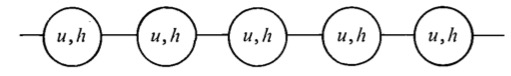
\includegraphics[keepaspectratio]{./pictest/pic411.jpg}}
\caption{}
\end{figure}

As far as the system \texttt{b1.5} is concerned, however, the underlined
variables in the figure depend only on other underlined variables. The
same statement holds for the variables that are not underlined. Thus,
the grid in the figure contains two elementary "subgrids", with the
solution on one of these subgrids being completely decoupled from the
other. Thus, it would be better to calculate only one of these
solutions, that is, to use a grid as shown in \texttt{figg:412}. Such a
grid, with variables carried at alternate points in space, is called a
\emph{staggered grid}. The computation time needed to solve
\texttt{b1.5} on the grid is reduced by a factor of two, and the
truncation error is the same. Furthermore, the waves with
\(k\Delta x > \frac{\pi}{2}\) have been eliminated, and these are just
the waves associated with large phase speed errors and negative group
velocities.

\begin{figure}
\centering
\pandocbounded{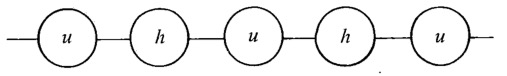
\includegraphics[keepaspectratio]{./pictest/pic412.jpg}}
\caption{}
\end{figure}

Thus, when using such a staggered grid, the phase speed and group
velocity diagram shown in \texttt{figg:14} of the preceding chapter is
reduced to its left half, covering waves with wave lengths of up to
\(4\Delta x\) only. This is a tremendous improvement.

If we wish to have waves with wave lengths between \(4\Delta x\) and
\(2\Delta x\) in our calculation we can reduce the grid length by a
factor of two and perform a much more accurate integration, using the
same amount of compu­tation time than with a grid that is not staggered.

\subsection{\texorpdfstring{\textbf{Two-dimensional gravity
waves}}{Two-dimensional gravity waves}}\label{Section4.2}

We now consider \emph{two-dimensional} gravity waves. Thus, we consider
the system of linearized equations

{\[\frac{\partial u}{\partial t} &= - g\frac{\partial h}{\partial x}\]\[\frac{\partial v}{\partial t} &= - g\frac{\partial h}{\partial y}\]\[\frac{\partial h}{\partial t} &= - H\nabla\cdot\textbf{v}\]}

Substituting the wave solutions

{\[u = Re\left\lbrack \widehat{u}e^{i\left( kx + ly - \nu t \right)} \right\rbrack\]\[v = Re\left\lbrack \widehat{v}e^{i\left( kx + ly - \nu t \right)} \right\rbrack\]\[h = Re\left\lbrack \widehat{h}e^{i\left( kx + ly - \nu t \right)} \right\rbrack\]}

We now obtain

{\[\nu^{2} = gH\left( k^{2} + l^{2} \right)\]}

Thus, in the two-dimensional case, the gravity waves propagate with the
same constant phase speed \(\sqrt{gH}\).

Because of the results obtained in the preceding section, we first
consider the spatial distribution of the variables. With two dimensions
and three dependent variables, a large number of spatial arrangements of
the variables are possible. For the present we consider the three
rectangular arrangements shown in \texttt{figg:421}. The identifying
letters (A), (E) and (C) are chosen so as to conform with the symbols
used by Winninghoff and Arakawa (Arakawa, 1972).

\begin{figure}
\centering
\pandocbounded{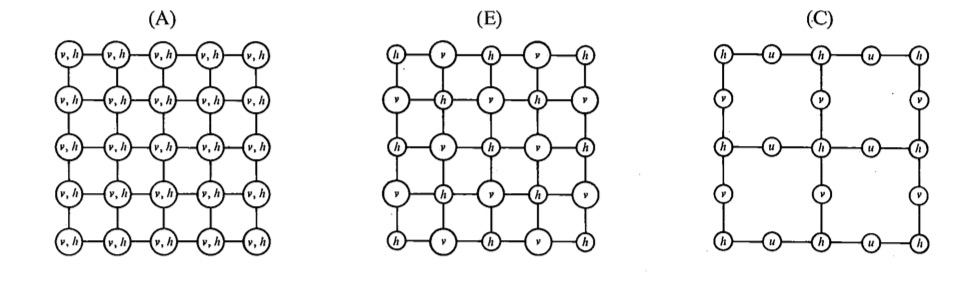
\includegraphics[keepaspectratio]{./pictest/pic421.jpg}}
\caption{}
\end{figure}

We shall denote the shortest distance between the grid points by
\(d^{*}\). With the same value of \(d^{*}\) the lattice (E) will have
twice, and the lattice (C) four times less variables per unit area than
the lattice (A), as in \texttt{figg:421}. The lattice (E) can be
obtained by a superposition of two (C) lattices, and the lattice (A) by
a superposition of two (E) lattices, or of four (C) lattices.

The admissible regions of wave numbers in the wave number plane can be
found by considering the shortest resolvable wave lengths. Note that
with lattice (E) the lines joining the nearest points with the same
variable make an angle of \(\frac{\pi}{4 }\) with the grid lines while
with the other two lattices these lines are along the grid lines.
\texttt{figg:422} shows the admissible wave numbers. A halving of the
number of variables is associated with a halving of the area of the
admissible region of the wave number plane.

The same standard finite difference approximations can be used for the
space derivatives in \texttt{b2.1} for all three lattices. We write
these approximations using the difference operators \(\delta_{x} \) and
\(\delta_{y}\), defined by, for example,

\[\delta_x h = \frac{1}{2d^*}\left[ h(x+d^*,y) - h(x-d^*,y)  \right]\]

Thus, \texttt{b2.1} can be approximated by

{\[\frac{\partial u}{\partial t} &= - g\delta_{x}h\]\[\frac{\partial v}{\partial t} &= - g\delta_{y}h\]\[\frac{\partial h}{\partial t} &= - H\left( \delta_{x}u + \delta_{y}v \right)\]}

Substituting wave solutions analogous as in \texttt{b2.2}, we obtain

{\[v^2 = gH\frac{\sin^{2}{kd^*} + \sin^2{l d^*}{d^{*2}}\]}

we define

\[X \equiv kd^{*} \qquad Y \equiv ld^{*}\]

\begin{figure}
\centering
\pandocbounded{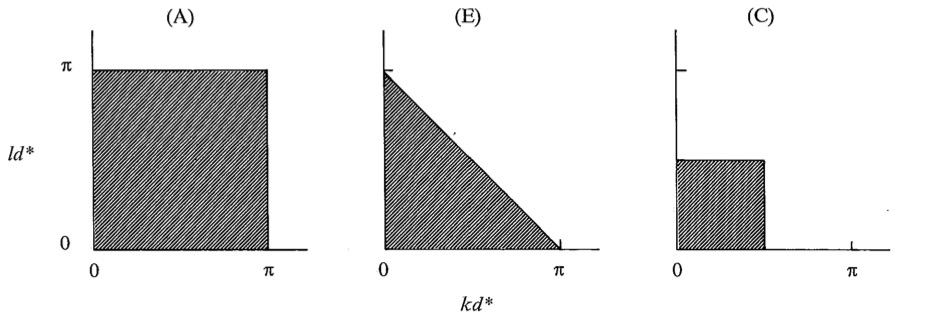
\includegraphics[keepaspectratio]{./pictest/pic422.jpg}}
\caption{}
\end{figure}

\begin{description}
\item[the ratio of the phase speed given by \texttt{b2.5}, \(c^*\) to
the true phase speed]
\(\sqrt{gH}\) , can be written as
\end{description}

{\[\frac{c^*}{ \sqrt{gH}} = \sqrt{\frac{\sin^{2}X + \sin^{2}Y}{X^{2} + Y^{2}}}\]}

This formula reduces to the previous formula, \texttt{b1.8} or
\texttt{b1.9}, when applied to the one-dimensional case.

The values of the relative phase speed \texttt{b2.6} on the wave number
region admitted by lattice (E) are shown in \texttt{figg:423}. By
symmetry about the line \(l = k\) only half of the region needs to be
shown. \texttt{figg:422} shows that lattice (C) admits only the left
half of the triangular region

\begin{figure}
\centering
\pandocbounded{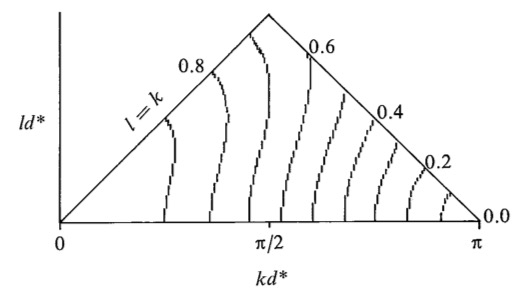
\includegraphics[keepaspectratio]{./pictest/pic423.jpg}}
\caption{}
\end{figure}

shown in the diagram. Clearly lattice (C) gives a more accurate phase
speed for gravity waves than the other lattices considered here.
Unfortunately, because it does not carry the two velocity components at
the same points, there is some difficulty with the Coriolis force term.
Of the other lattices, the staggered lattice (E) is much superior to the
non-staggered lattice (A). A result with the same truncation error can
be achieved in about half of the computation time, (exactly half if the
equations are linear), and a sizable fraction of wave numbers that are
associated with large phase speed errors and compu­tational dispersion
are eliminated. The additional time needed for a calculation on an (A)
lattice is spent on waves that can hardly be expected to improve the
inte­gration.

As we can see from the phase speed diagram, lattice (E) is not free of
computational problems.

As with the non-staggered one-dimensional grid discussed in the
preceding section, the solutions of \texttt{b2.4} on each of the two
type (C) subgrids forming the (E) lattice are inde­pendent and can
diverge from each other. This can be a source of serious problems. For
example, if the values of the dependent variables on one of these (C)
lattices are constant, they will be a stationary solution on that
lattice, no matter what the values of the variables on the other (C)
lattice are. Two stationary solutions, with different constant values on
each of these complementary lattices, will give a stationary wave
represented by the right-hand corner of the triangular region in
\texttt{figg:423}, with a zero phase speed. This wave is usually
referred to as the \emph{two-grid-interval wave}. In the same way, the
(A) lattice admits four independent stationary solutions, with different
constant values on each of its four type (C) subgrids.

The two-grid-interval wave can easily be generated when boundary
conditions are artificially described, and, with more complete
equations, in cases when gravity waves are generated inside the
computational region. These can be caused by heating, for example
through the release of latent heat, and by the influence of mountains.
When gravity waves are excited involving variables of one of the (C)
subgrids only, for example by forcing at individual grid points or lines
of points, the gravity wave will propagate through the variables of this
subgrid only. The variables of the other (C) subgrid will be influenced
only through the Coriolis and advection terms on a much larger
time-scale. Thus physical effects which may excite relatively long waves
in the atmosphere may excite spurious waves with wave lengths of
approximately two grid intervals in a computation. When these reach an
excessive amplitude, some remedial measures have to be taken. These will
be discussed in a later section.

\subsection{\texorpdfstring{\textbf{Gravity-inertia waves and space
distribution of
variables}}{Gravity-inertia waves and space distribution of variables}}\label{Section4.3}

In this section we discuss the effect of centered space differencing on
\emph{gravity-inertia waves}. Thus, we consider the system of linearized
equations

{\[\frac{\partial u}{\partial t} &= - g\frac{\partial h}{\partial x} +f v\]\[\frac{\partial v}{\partial t} &= - g\frac{\partial h}{\partial y} - f u\]\[\frac{\partial h}{\partial t} &= - H\nabla\cdot\textbf{v}\]}

These equations differ from those of section \texttt{Section4.2} in the
appearance of the two Coriolis terms. The Coriolis terms contain no
derivatives. However, they are difficult to calculate on the (C)
lattice, which was ideal for pure gravity waves.

Thus, we reconsider the problem of the distribution of the variables.

It is not obvious how we should analyse various arran­gements of
variables. Our primary concern here is to consider \texttt{b3.1} as part
of the complete system of primitive equations. We are interested in
large-scale motions, otherwise we would not be including the Coriolis
terms.

On the large scale, the primitive equations admit two district types of
motion : low-frequency, quasi-geostrophic and quasi-nondivergent flow
and high-frequency gravity-inertia waves. Gravity-inertia waves are
continually excited in the atmosphere. However, as they are dispersive,
a local accumulation of wave energy disperses with time. This process is
known as geostrophic adjustment; the remaining motion is in approximate
geostrophic balance and changes only slowly in time. In this chapter we
are concerned with the correct simulation of this process, which is
essentially governed by the gravity-inertia wave equations
\texttt{b3.1}.

We are interested both in waves caused by physical effects, and in those
caused by inadequacies of the initial data and of the numerical
procedures.

However, the details of the adjustment process do not matter as much as
the correctness of the resulting quasi-geostrophic flow.

We shall therefore investigate the effect of the space distribution of
dependent variables on the dispersive properties of the gravity-inertia
waves. This will be done using the simplest centered approximations for
the space derivatives, leaving the time derivatives in their
differen­tial form.

The discussion is based on that by Winninghoff and Arakawa, as presented
by Arakawa (Arakawa, 1972; Arakawa et al. 1974).

We consider five ways of distributing the dependent variables in space,
shown in \texttt{figg:431}. We denote by \emph{d} the shortest distance
between neighbouring points carrying the same dependent variable. In the
figure \emph{d} is the same for each of the five lattices ; thus, all
the lattices have \emph{the same number of dependent variables per unit
area}. The computation time needed for an integration on each of the
lattices will be about the same; the properties of the solution
obtained, though, will differ because of the effect of the space
arrangement of variables.

Using the subscripts shown in the figure, we define the centered space
differencing operator by

\[(\delta_x\alpha) = \frac{1}{d'} \left( \alpha_{i+\frac{1}{2},j} - \alpha_{i-\frac{1}{2},j} \right)\]

this rotation is applicable to all the lattices. Here \(d^{'}\) is the
distance between the points between which the finite difference is
taken. Thus, for lattices (A) through (D) \(d^{'}\) is equal to the grid
size \(d\), and for the lattice (E) it is equal to \(\sqrt{2d}\).

\begin{figure}
\centering
\pandocbounded{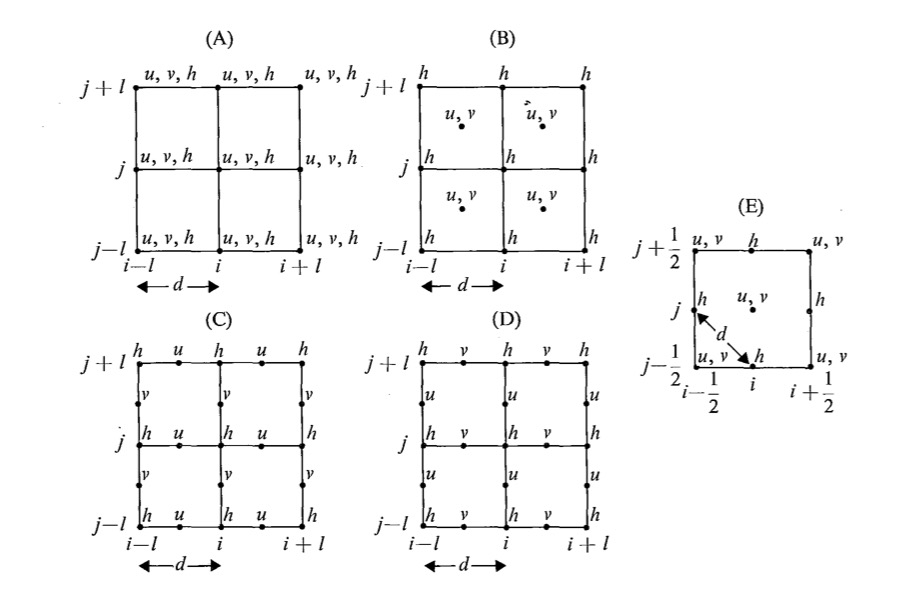
\includegraphics[keepaspectratio]{./pictest/pic431.jpg}}
\caption{}
\end{figure}

We also define an average taken over the same two points by

\[\left( {\overline{\alpha}}^{x} \right)_{i,j} \equiv \frac{1}{2}\left( \alpha_{i + \frac{1}{2},j} - \alpha_{i - \frac{1}{2},j} \right)\]

\(\left( \delta_{y}\alpha \right)_{i,j}\) and
\(\left( {\overline{\alpha}}^{y} \right)_{i,j}\) are defined in the same
way, but with respect to the \emph{y} axis. Finally,

\[\left( {\overline{\alpha}}^{xy} \right)_{i,j}  \equiv  \left( {\overline{\overline{\alpha}}^{x}}^y \right)_{i,j}\]

For each of the five lattices we use the simplest centered
approximations for the space derivatives and Coriolis terms
\texttt{b3.1}. We obtain the difference systems

{\[\frac{\partial u}{\partial t} &= - g\overline{\delta_x h}^{x} + fv\]\[\frac{\partial v}{\partial t} &= - g\overline{\delta_y h}^{y} - fu\]\[\frac{\partial h}{\partial t} &= -H\left( \overline{\delta_x u}^{x} + \overline{\delta_y v}^{y} \right)\]}

{\[\frac{\partial u}{\partial t} &= - g\overline{\delta_x h}^{y} + fv\]\[\frac{\partial v}{\partial t} &= - g\overline{\delta_y h}^{x} - fu\]\[\frac{\partial h}{\partial t} &= -H\left( - \overline{\delta_x u}^{y} +  \overline{\delta_y v}^x \right)\]}

{\[\frac{\partial u}{\partial t} &= - g\delta_x h + f\overline{v}^{xy}\]\[\frac{\partial v}{\partial t} &= - g\delta_y h - f\overline{u}^{xy}\]\[\frac{\partial h}{\partial t} &= -H\left( \delta_x u +  \delta_y v \right)\]}

{\[\frac{\partial u}{\partial t} &= - g\overline{\delta_x h}^{xy} + f\overline{v}^{xy}\]\[\frac{\partial v}{\partial t} &= - g\overline{\delta_y h}^{xy} - f\overline{u}^{xy}\]\[\frac{\partial h}{\partial t} &= -H\left( \overline{\delta_x u}^{xy} 
+  \overline{\delta_y v}^{xy} \right)\]}

{\[\frac{\partial u}{\partial t} &= - g\delta_x h + fv\]\[\frac{\partial v}{\partial t} &= - g\delta_y h - fu\]\[\frac{\partial h}{\partial t} &= -H\left( \delta_x u +  \delta_y v \right)\]}

We shall first analyze a one-dimensional case, that in which the
variables, \(u,v \) and h do not vary with \(y\)

Thus, we have

\begin{quote}
\(u,v,h = u,v,h\left( x,t \right)\)
\end{quote}

The system \texttt{b3.1} then reduces to

{\[\frac{\partial u}{\partial t} &= -g\frac{\partial h}{\partial x} + fv\]\[\frac{\partial v}{\partial t} &= - fu\]\[\frac{\partial h}{\partial t} &= -H\frac{\partial u}{\partial x}\]}

Substituting the wave solutions \texttt{b1.2}, we obtain the frequency
equation which can be written as

{\[\left( \frac{\nu}{f} \right)^{2} = 1 + \frac{gH}{f^{2}}k^{2}\]}

Thus, as the \emph{radius of deformation}

\[\lambda = \sqrt{\frac{gH}{f}}\]

is never equal to zero, the frequency of the gravity-inertia waves is a
monotonically increasing function of \(k\). Therefore, the group
velocity \(\frac{\partial\nu}{\partial k}\) is never equal to zero. This
is very important for the geostrophic adjust­ment process, as it
precludes a local accumulation of wave energy.

We now look at the effect of the finite differencing in space in this
case. As the variables are assumed not to depend on \(y\), the systems
\texttt{b3.2A} reduce to

{\[\frac{\partial u}{\partial t} &= - g\overline{\delta_x h}^{x} + fv\]\[\frac{\partial v}{\partial t} &=  - fu\]\[\frac{\partial h}{\partial t} &= -H \overline{\delta_x u}^{x}\]}

{\[\frac{\partial u}{\partial t} &= - g\delta_x h + fv\]\[\frac{\partial v}{\partial t} &=  - fu\]\[\frac{\partial h}{\partial t} &= -H \delta_x u\]}

{\[\frac{\partial u}{\partial t} &= - g\delta_x h + f\overline{v}^{x}\]\[\frac{\partial v}{\partial t} &=  - f\overline{u}^{x}\]\[\frac{\partial h}{\partial t} &= -H \delta_x u\]}

{\[\frac{\partial u}{\partial t} &= - g\overline{\delta_x h}^{x} + f\overline{v}^{x}\]\[\frac{\partial v}{\partial t} &=  - f\overline{u}^{x}\]\[\frac{\partial h}{\partial t} &= -H \overline{\delta_x u}^{x}\]}

{\[\frac{\partial u}{\partial t} &= - g\delta_x h + fv\]\[\frac{\partial v}{\partial t} &=  - fu\]\[\frac{\partial h}{\partial t} &= -H \delta_x u\]}

Substitution of wave solutions into these systems gives the frequency
equations

{\[\left(\frac{\nu}{d}\right)^2 = 1 + \left(\frac{\lambda}{d}\right)^2 \sin^2{kd}\]}

{\[\left(\frac{\nu}{d}\right)^2 = 1 + 4\left(\frac{\lambda}{d}\right)^2 \sin^2{\frac{kd}{2}}\]}

{\[\left(\frac{\nu}{d}\right)^2 = \cos^2{\frac{kd}{2}} + 4\left(\frac{\lambda}{d}\right)^2 \sin^2{\frac{kd}{2}}\]}

{\[\left(\frac{\nu}{d}\right)^2 = \cos^2{\frac{kd}{2}} + \left(\frac{\lambda}{d}\right)^2 \sin^2{\frac{kd}{2}}\]}

{\[\left(\frac{\nu}{d}\right)^2 = 1 + 2\left(\frac{\lambda}{d}\right)^2 \sin^2{\frac{kd}{\sqrt{2}}}\]}

The non-dimensional frequency \(\frac{\nu}{f}\) is now seen to depend on
two parameters, \(kd\) and \(\frac{\lambda}{d}\)

We shall analyze the dispersion properties revealed by these expressions
for each of the five lattices. The wavelength of the shortest resolvable
wave along the \(x\) axis is \(2d\) for lattices (A) through (D), and
\(\sqrt{2d}\) for the lattice (E). Thus, we have to consider the range
\(0 < kd \leq \pi\) for lattices (A) through (D), and the range
\(0 < kd \leq \sqrt{2\pi}\) for the lattice (E).

Lattice (A): The frequency reaches a maximum a \( kd = \frac{\pi}{2}\)
Thus, the group velocity is zero for \(k\) equal to
\(\frac{\pi}{\left( 2d \right)}\). If gravity-inertia waves of
approximately that wave number are excited near a point inside the
computa­tional region, for example by nonlinear effects or forcing
through heating or ground topography, the wave energy stays near that
point. Beyond this maximum value, for \(\frac{\pi}{2 < kd < \pi}\), the
frequency decreases as the wave number increases. Thus, for these waves
the group velocity has the wrong sign. Finally, the two-grid-interval
wave with \(kd = \pi\) behaves like a pure inertia oscillation, and its
group velocity is again zero.

Lattice (B): The frequency increases monotonically throughout the range
\(0 < kd < \pi\) . However, it reaches a maximum at the end of the
range, so that the group velocity is zero for the two-grid-interval wave
with \(kd = \pi.\)

Lattice (C): The frequency increases monotonically with \(\text{kd}\) if
\(\frac{\lambda}{d} > \frac{1}{2} \) and decreases monotonically with
\(\text{kd}\) if \(\frac{\lambda}{d} < \frac{1}{2}\). It again reaches
an extreme value at \(kd = \pi\), associated with a zero group velocity.
For \(\frac{\lambda}{d} = \frac{1}{2}\) the group velocity is equal to
zero for all \(k\) .

Lattice (D): The frequency reaches a maximum at
\(\left( \frac{\lambda}{d} \right)^{2}\cos{kd} = \frac{1}{4}\). The
two-grid-interval wave at \(kd = \pi\) is stationary.

Lattice (E): The frequency reaches a maximum at
\(kd = \frac{\pi}{\sqrt{2}}\). The shortest resolvable wave with
\(kd = \sqrt{2\pi}\) behaves like a pure inertia oscillation, and its
group velocity is again zero.

A summary of these results is shown in \texttt{figg:432}. It shows the
functions \(\frac{|v|}{f}\), in the case \(\frac{y}{d} = 2\).

\begin{figure}
\centering
\pandocbounded{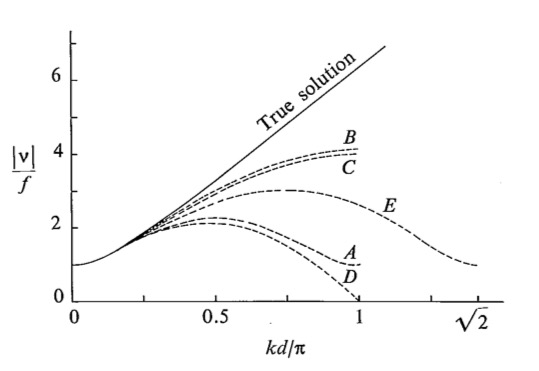
\includegraphics[keepaspectratio]{./pictest/pic432.jpg}}
\caption{}
\end{figure}

The figure vividly illustrates the inadequacy of the lattices (D) and
(A). The phase speed and dispersion properties of the remaining three
lattices are much better: however, zero group velocities occur with
every lattice. Thus, with any lattice there will be difficulties in the
geostrophic adjustment process.

The difference between the results for lattices (B) and (E) is
interesting because these two lattices can be obtained from one another
by a rotation through an angle of \(\frac{\pi}{4}\) If we consider the
one-dimensional case in which the dependent variables are constant along
the lines \(y = x + c\), we obtain results for these two lattices that
are exactly opposite to those in\texttt{figg:432}. In general, we define
the coordinate system \emph{x\textquotesingle, y\textquotesingle{}} by
rotating the \emph{x,y} in the positive direction through an angle of
\(\frac{\pi}{4}\), and then, using the relations

\[u^{'} &= \frac{\sqrt{2}}{2}\left( u + v \right)\]\[v^{'} &= \frac{\sqrt{2}}{2}\left( - u + v \right)\]

change from variables \(u,v,h\) to new dependent variables
\(u^{'},v^{'},h\) . We find that this transforms the system
\texttt{b3.2B} into \texttt{b3.2E}, and, conversely, \texttt{b3.2E} into
\texttt{b3.2B}. Thus, the \emph{dispersion properties of the lattices
(B) and (E) can be considered equivalent}. A gravity-inertia wave in one
of these lattices has phase speed and dispersion properties identical to
those of the same wave with its front rotated through an angle of
\(\frac{\pi}{4}\) in the other lattice.

Obviously, we should also consider the two-dimensional case. The values
of \(\frac{|v|}{f}\) that are obtained in the two-dimensional case for
the true solution and those using lattices (B) and (C) are shown in
\texttt{figg:433} with \(\frac{\lambda}{d'} = 2\). The diagram for
lattice (E) can be obtained by a counter­clockwise rotation of the (B)
lattice diagram.

\begin{figure}
\centering
\pandocbounded{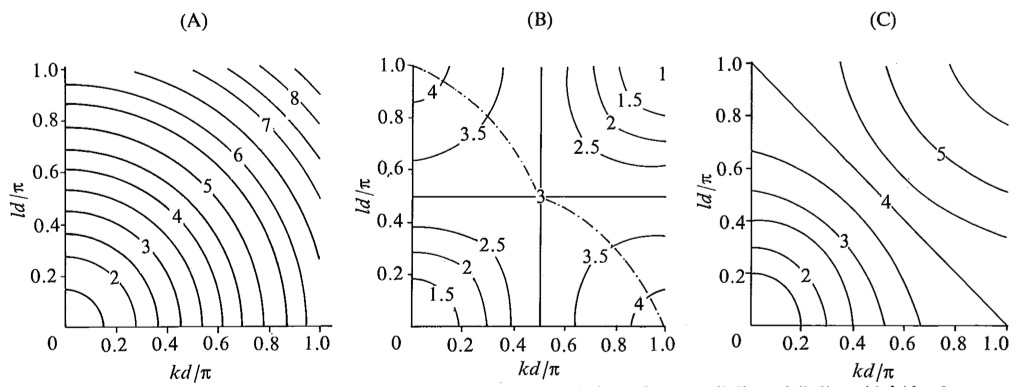
\includegraphics[keepaspectratio]{./pictest/pic433.jpg}}
\caption{}
\end{figure}

The diagram for lattice (C) in the two-dimensional case is seen to be a
much better approximation to the exact solution than the (B) or (E)
lattice diagram. In the (B) lattice diagram the dot-dashed line shows
the maximum \(\frac{|v|}{f}\) for a given ratio \(\frac{l}{k}\); note
that there is no such line in the (C) lattice diagram and the exact
solution. Such a maximum occurs at only two corner points of the (C)
lattice diagram. Thus, with the (C) lattice, no waves have a group
velocity with the wrong sign. The situation, though, does depend on the
parameter \(\frac{\lambda}{d}\). With a stra­tified atmosphere the
radius of deformation \(\lambda\). depends on the stability ; if the
stability is so weak as to make \(\frac{\lambda}{d}\) of the order of 1
or less, the (C) lattice loses the advantages shown in
\texttt{figg:433}. However, for typical grid sizes used in atmospheric
models this is not the case and therefore Arakawa (Arakawa and Lamb,
1976) concludes that the lattice (C) is the best lattice to simulate the
geostrophic adjustment process. Accordingly, it is at present being used
in the general circulation model at the University of California at Los
Angeles, and also in the British operational model.

The (B) or (E) lattices have a problem with false low frequencies of the
shortest waves. The two-grid-interval wave, that was stationary as a
pure gravity wave, now behaves like a pure inertia oscillation. The
difficulty arises from decoupling of the gravity wave solutions on the
two complementary (C) type subgrids. Methods of dealing with this will
be discussed later.

\subsection{\texorpdfstring{\textbf{Time differencing; the leapfrog
scheme and the Eliassen
grid}}{Time differencing; the leapfrog scheme and the Eliassen grid}}\label{Section4.4}

Properties of time differencing schemes applied to the gravity wave
equations can be deduced from the analysis of Chapter \texttt{Chapter2},
as was done for the advection equation.

We shall demonstrate this for the one-dimensional equations

{\[\frac{\partial u}{\partial t} + c\frac{\partial u}{\partial x} +
 g\frac{\partial h}{\partial x} &= 0\]\[\frac{\partial h}{\partial t} + c\frac{\partial h}{\partial x} +
 H\frac{\partial u}{\partial x} &= 0\]}

We first multiply the second of these equations by an arbitrary
parameter \(\lambda\), and add the result to the first equation. We
obtain

{\[\frac{\partial}{\partial t}( u + \lambda h ) +
( c + \lambda H )\frac{\partial u}{\partial x} +
( g + \lambda c )\frac{\partial h}{\partial x} = 0\]}

We wish to choose \(\lambda\) so that

{\[\frac{g + \lambda c}{c + \lambda H} = \lambda\]}

\begin{description}
\item[to obtain an equation with only one dependent variable,]
\(u + \lambda h\) . The two solutions of \texttt{b4.3} are
\end{description}

{\[\lambda = \pm \sqrt{\frac{g}{H}}\]}

Substituting these into \texttt{b4.2} we obtain

{\[\left[ \frac{\partial}{\partial t} + ( c + \sqrt{gH}\frac{\delta}{\text{δx}} ) \right] \left( u + \sqrt{\frac{g}{H}}h \right) &= 0\]\[\left[ \frac{\partial}{\partial t} + ( c - \sqrt{gH}\frac{\delta}{\text{δx}} ) \right] \left( u - \sqrt{\frac{g}{H}}h \right) &= 0\]}

This is the \emph{normal form} of the system \texttt{b4.1}. It shows
that \texttt{b4.1} is equivalent to a system of two advection
equations*. The quantity \(u + \sqrt{\frac{g}{H}}h\) is seen to be
advected at a velocity \(c + \sqrt{gH}\) in the direction of the
\(\text{x }\) axis, while, at the same time, the quantity
\(u - \sqrt{\frac{g}{H}}h\) is advected in the same direction at a
velocity \(c - \sqrt{gH}\).

Suppose now we choose a grid that carries both u and h at every grid
point. The systems obtained by using centered space differencing in
\texttt{b4.1} and \texttt{b4.5} are then equivalent. We can therefore
use the same procedure as in Section 1 of the Chapter \texttt{Chapter3}
to analyse time differencing schemes. We obtain the same results as
before, except that in place of the advection velocity \(c\) we now have
\(c + \sqrt{gH}\). Thus, if the \emph{leapfrog scheme} is used for the
time differencing, and \(c\) is considered positive, we obtain the
Courant-Friedrichs-Lewy stability criterion for this case as

{\[( c + \sqrt{gH})\frac{\Delta t}{\Delta x} \leq 1\]}

The advection velocity in the atmosphere is normally about an order of
magnitude less than the phase speed of external gravity waves.
Accordingly, in the foregoing criterion \(c\) is often neglected
compared with \(\sqrt{gH}\), giving the stability requirement

{\[\sqrt{gH}\frac{\Delta t}{\Delta x} < 1\]}

When using the \emph{three-dimensional} primitive equations, external
gravity waves are normally eliminated by per­mitting no vertical
velocity at the upper boundary. The highest phase speed admitted by the
system is then that of the Lamb waves, which for an isothermal
atmosphere is

\[\sqrt{\left( \frac{f}{k} \right)^{2} + \gamma RT}\]

where \(\gamma \equiv \frac{c_{p}}{c_{v}}\). If we neglect the first
term and recall that the scale height of an isothermal atmosphere is

\[H^{*} = \frac{RT}{g}\]

we see that the phase speed of the Lamb waves is of the same order of
magnitude as that of the external gravity waves. Thus, in view of the
relation between stability and the phase speed, we see that
\texttt{b4.7} should also repre­sent an approximately correct stability
requirement in the three-dimensional case. With the highest phase speeds
of the order of 300 m \(\text{sec}^{-1}\), and a grid size of about 100
km, this requirement does not permit time steps longer than about 5
minutes. This time will be smal­ler by a factor of \(\sqrt{2}\) with two
horizontal coordinates. The CFL stability condition thus means that a
large amount of computer time is required for integration of the
primitive equations, especially when the grid size is small to reduce
errors in space differencing. For this reason some investigators prefer
using implicit time dif­ferencing schemes, so that the choice of time
step can be based solely on accuracy and not on stability.

We can also study the stability and other properties of time
differencing methods applied to the gravity wave equations by direct
substitution of wave solutions. For example, consider the leapfrog
scheme with centered space differencing applied to the
\emph{two-dimensional} system

{\[\frac{\partial u}{\partial t} + g\frac{\partial h}{\partial x} = 0\]\[\frac{\partial v}{\partial t} + g\frac{\partial h}{\partial y} = 0\]\[\frac{\partial h}{\partial t} + H\nabla\cdot v = 0\]}

Using one of the lattices of \texttt{figg:421} as well as the notation
of Section \texttt{Section4.2}, we obtain

{\[u^{n+1} = u^{n-1} -2 g \Delta t \delta_x h^n\]\[v^{n+1} = v^{n-1} -2 g \Delta t \delta_y h^n\]\[h^{n+1} = h^{n-1} -2 H \Delta t ( \delta_x u + \delta_y v)^n\]}

Substituting the wave solutions

{\[u^n = Re \left[ \lambda^n \widehat{u} e^{i(kx+ly)} \right]\]\[v^n = Re \left[ \lambda^n \widehat{v} e^{i(kx+ly)} \right]\]\[h^n = Re \left[ \lambda^n \widehat{h} e^{i(kx+ly)} \right]\]}

we obtain the homogeneous system

{\[\left( \lambda^{2} - 1 \right)\widehat{u} + i\lambda 2\sqrt{2}g\mu \sin{X}\widehat{h} = 0\]\[\left( \lambda^{2} - 1 \right)\widehat{v} + i\lambda 2\sqrt{2}g\mu \sin{Y}\widehat{h} = 0\]\[i\lambda 2\sqrt{2}K\mu \left( \sin{X}\widehat{u} + \sin{Y}\widehat{v} \right) + \left( \lambda^{2} - 1 \right)\widehat{h} = 0\]}

Here \emph{X} and \emph{Y} are defined as in Section \texttt{Section4.2}
, while

\[\mu \equiv \frac{\Delta t}{\left( \sqrt{2}d^{*} \right)}\]

that is, \(\mu \equiv \frac{\Delta t}{d}\) when the lattice (E) is
chosen.

The properties of the numerical solution can now be studied by analyzing
\texttt{b4.11}. The requirement that its determinant be equal to zero
gives six solutions for \(\lambda\). Two of these are

{\[\lambda = 1\]}

and

{\[\lambda = - 1\]}

The remaining four are given by

{\[\lambda^{2} = 1 - 4A \pm 2\sqrt{2A( 2A - 1 )}\]}

Where

\[A \equiv gH\mu^{2}\left( \sin^{2}X + \sin^{2}Y \right)\]

We can now analyze the solutions \texttt{b4.10} associated with the
values found for \(\lambda\). The first of these values, \texttt{b4.12},
gives a neutral and stationary solution. If either \(\sin{X}\) or
\(\sin{Y}\) is non-zero in this neutral and stationary case then,
according to \texttt{b4.11}, we have \(\widehat{h} = 0\), and the
solution represents a physically acceptable translatory motion. If,
however, sin \(X\) and \(\sin{Y}\) are both equal to zero, the
amplitudes of all three dependent variables can take arbitrary values.
In addition to the physically acceptable solution where all the
dependent variables are constant \(\left( k = l = 0 \right)\) there is a
solution with one or both of the wave numbers \(k\) and \(l\) equal to
\(\frac{\pi}{d^{*}}\). This is the two-grid-interval wave, discussed
already in Section \texttt{Section4.2}. It again appears as a false
computational solution; since it is stationary, it is not affected by
the introduction of time differencing.

The second value, \(\lambda = - 1\), represents a false compu­tational
mode in time, with a period of \(2\Delta t\). This com­putational mode
results from using a three time level scheme.

To prove stability of the scheme the behaviour of the remaining
solutions given by \texttt{b4.14} has to be investigated. They will all
also be neutral for \(2A < 1\). To obtain the condition in the form
\(B\Delta t \leq 1\) we write

\[\sqrt{2A \leq 1}\]

Since this has to be satisfied for all the admissible waves, we find
that the CFL criterion in the two-dimensional case is now

{\[2\sqrt{gH}\mu \leq 1\]}

or

{\[\sqrt{2gH}\frac{\Delta t}{\Delta x} \leq 1\]}

This is in agreement with the previous results. The non dimensional
constant on the left side is sometimes called the \emph{Courant number}.

With solutions like \texttt{b4.10}, the frequency \(\text{v }\) is given
by

\[\lambda = \left| \lambda \right|e^{- i\nu\Delta t}.\]

Thus, the expressions obtained for \(\lambda\) can be used to calcu­late
the \emph{relative phase speed} \(\frac{c^{*}}{\sqrt{gH}}\) using the
relation

{\[\frac{c^{*}}{\sqrt{gH}} = \frac{1}{\Delta t\sqrt{gH\left( k^{2} + l^{2} \right)}}\arctan\frac{- \lambda_{im}}{\lambda_{re}}\]}

If we are given \(\lambda^{2}\) rather than \(\lambda\), as here, we can
express the relative phase speed as a function of \((\lambda^{2})_{im}\)
and \((\lambda^{2})_{re}\). Thus, using \texttt{b4.14}, we find for
\(2A \leq 1:\)

{\[\frac{c^*}{\sqrt{gH}} = \frac{1}{2\mu\sqrt{2gH\left( X^{2} + Y^{2} \right)}} \times
 \arctan{ \left( \pm \frac{2\sqrt{2A\left( 1 - 2A \right)}}{1 - 4A} \right)   }\]}

\begin{description}
\item[This expression, of course, approaches \texttt{b2.6} as]
\(\Delta t\) approaches zero.
\end{description}

For a more explicit illustration of the effect of time differencing, we
can perform a series expansion of \texttt{b4.18}. One obtains, for
\(\sqrt{2A} < \frac{1}{\sqrt{2}},\)

\[\frac{c^*}{\sqrt{gH}} = 
\sqrt{\frac{\sin^2{X} + \sin^2{Y}}{X^2 + Y^2}} \left( 1 + \frac{1}{3}A + \frac{3}{10}A^2 + \ldots \right)\]

The factor multiplying the series in parenthesis describes the
decelerating effect of space differencing, as given by \texttt{b2.6}.
The acceleration resulting from the leapfrog time differencing is
beneficial, as it reduces the phase error due to space differencing.

The values of the relative phase speed \texttt{b4.18} are shown in
\texttt{figg:441}, for the physical mode with \( 2\sqrt{gH\mu} = 0.5\).
The wave number region shown here is the same as in \texttt{figg:423},
where the effect of space differencing alone was considered. Comparison
of these figures shows little difference between the two families of
isolines. The relative acceleration due to the time differencing has a
maximum at the upper corner of the diagram, but the relative phase speed
here is still poor.

\begin{figure}
\centering
\pandocbounded{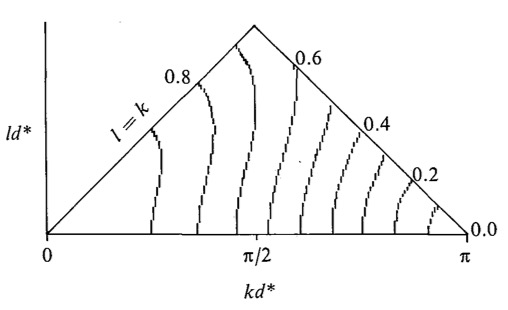
\includegraphics[keepaspectratio]{./pictest/pic441.jpg}}
\caption{}
\end{figure}

Finally, we point out that time differencing suggests new ways of
distributing the variables, as the grid can now also be time-staggered.
A good example is given by the linearized system

{\[\frac{\partial u}{\partial t} + g\frac{\partial h}{\partial x} - fv &= 0\]\[\frac{\partial v}{\partial t} + g\frac{\partial h}{\partial y} + fu &= 0\]\[\frac{\partial h}{\partial t} + H\left( \frac{\partial u}{\partial x} + \frac{\partial v}{\partial y}  \right) &= 0\]}

approximated using lattice (E), the leapfrog scheme and centered space
differencing. If all the variables were calculated at every time level,
there would be two inde­pendent solutions. The solution involving the
variables of the space-time grid shown in \texttt{figg:442} would be
indepen­dent of that involving the variables that are left out in this
figure. The second grid can be obtained by shifting the grid a distance
\(\sqrt{2d^{*}} \) along the line \( y = x.\) Thus, as with the space
grids discussed in Section \texttt{Section4.2}, the space-time grid
formed by using the (E) lattice at every time level can be considered as
a superposition of two element­ary subgrids of the type shown in
\texttt{figg:442}. Solving the system \texttt{b4.19} on only one of
these saves half the computa­tion time, with no change in the truncation
error. In addition the computational mode in time, given by
\texttt{b4.13}, is eliminated, as the variables at alternate time levels
are missing. Thus, with a more complete system of equations, the gradual
separation of solutions at alternate time levels is not possible. The
advantages of the space-time grid shown in the figure were pointed out
by Eliassen (1956) at an early stage in the study of the primitive
equations, and it is called the \emph{Eliassen grid.}

However, as pointed out by Platzman (1958 ; 1963) the grid in
\texttt{figg:442} can again be considered as formed by a superposition
of two subgrids, where in each of these subgrids only the height is kept
at one time level and the velocity components at the next. Platzman
calls this sub­grid the \emph{Richardson grid}. A single Richardson grid
is considered as a time-staggered version of the (C) lattice and
suffices for the solution of the pure gravity wave system \texttt{b4.9}
; thus, on an Eliassen grid the system \texttt{b4.9} has two independent
solutions. Using the difference system considered above to approximate
the differential system \texttt{b4.19}, these solutions are coupled only
through the two Coriolis terms.

\begin{figure}
\centering
\pandocbounded{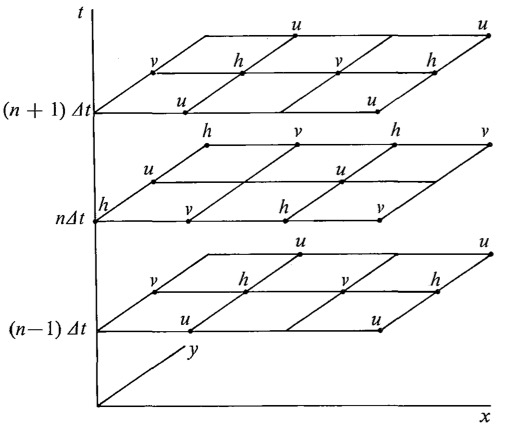
\includegraphics[keepaspectratio]{./pictest/pic442.jpg}}
\caption{}
\end{figure}

\subsection{\texorpdfstring{\textbf{Economical explicit
schemes}}{Economical explicit schemes}}\label{economical-explicit-schemes}

The fact that we are now solving two equations, the equation of motion
and the continuity equation, sug­gests new ways of constructing time
differencing sche­mes. Some of these have recently attracted the
attention of atmospheric modellers.

As seen in the section \texttt{Section4.4}, an inconvenient feature of
gravity waves is the high computer time required for a solution using
explicit schemes for the time differencing. The time step imposed by the
CFL stability criterion is generally considered to be much less than
that required for an accurate integration of the slower
quasi-geostro-phic motions. With these steps, the errors due to space
differencing are much greater than those due to time differencing.
Robert (1974), for example, estimates that the typical errors due to
space differencing in present atmospheric models amount to nearly 40 per
cent, and those due to time differencing only to about 1 per cent of the
total error. Thus, any economy that can be made in time differencing is
welcome, as the time that is saved can usefully be used to increase the
accuracy of the space differencing.

Two explicit schemes that are more economical than the standard leapfrog
scheme will be given here. They both achieve economy by using a
different integration procedure for the height gradient terms of the
equation of motion and for the divergence term of the continuity
equation. For brevity, we call these terms the \emph{gravity wave terms}
of the governing equations.

We shall discuss the properties of one of these "econo­mical" schemes in
some detail. It is obtained by first integrating the gravity wave terms
of \emph{either} the equation of motion or of the continuity equation
forward, and then those of the other equation backward in time. Thus,
this scheme could be called the \emph{forward-backward} scheme. With
centered space differencing, \texttt{b4.8} is approximated by

{\[u^{n + 1} = u^{n} - g\Delta t\delta_{x}h^{n}\]\[v^{n + 1} = v^{n} - g\Delta t\delta_{y}h^{n}\]\[h^{n + 1} = h^{n} - H\Delta t\left( \delta_{x}u + \delta_{y}v \right)^{n + 1}\]}

or by an analogous system in which the order of integra­tion is
reversed.

Substituting the wave solutions \texttt{b4.10} we find three solutions
for x. One of these,

{\[\lambda = 1\]}

gives again a neutral and stationary solution. The remaining two are

{\[\lambda = 1 - A \pm \sqrt{A\left( A - 2 \right)}\]}

where the quantity \(A\) is defined as in the preceding section.
Solutions \texttt{b5.2} and \texttt{b5.3} are obtained for both versions
of the scheme, that is, no matter which of the two equations — the
equation of motion or the conti­nuity equation — is first integrated
forward.

Examination of the amplification factors given by \texttt{b5.3} shows
that the scheme is stable and neutral for \(  A \leq 2\) , that is, for

\[\sqrt{2A} \leq 2\]

To satisfy this for all the admissible waves, we must have

{\[2\sqrt{gH} \mu \leq 2\]}

Thus, the forward-backward scheme is stable and neutral with time steps
\emph{twice those allowed by the CFL criterion for the leapfrog scheme}
(Ames, 1969).

The amplification factors of the forward-backward and of the leapfrog
scheme are equal within their regions of stability. We now compare their
effect on the phase speed by comparing the expression \texttt{b5.3}, for
the forward­backward scheme, with \texttt{b4.14}, for the leapfrog
scheme. The right-hand side of \texttt{b5.3}, with \(A\) replaced by
\(4A\), is equal to the right-hand side of \texttt{b4.14}. Because of
the definition of \(A\), this means that \(\lambda\) for the
forward-back­ward scheme is identical to \(\lambda^{2}\) for the
leapfrog scheme when time steps are used for the forward-backward scheme
\emph{twice as long as} those for the leapfrog scheme ! Thus, the
forward-backward scheme gives the same result using only half the
computation time needed for the leapfrog scheme. In addition, as a two
level scheme, it has no computational mode in time.

To understand this advantage of the forward-back­ward over the leapfrog
scheme we compare the finite difference analogues that these two schemes
give for the wave equation, since the system of gravity wave equa­tions
is equivalent to a single wave equation. Consider the one-dimensional
version of this system:

{\[\frac{\partial u}{\partial t} + g\frac{\partial h}{\partial x} = 0\]\[\frac{\partial h}{\partial t} + H\frac{\partial u}{\partial x} = 0\]}

Eliminating one of the variables u, h we obtain a wave equation

{\[\frac{\partial^{2} h}{\partial t^{2}} - gH\frac{\partial^{2} h}{\partial x^{2}} = 0\]}

We can perform the same elimination for each of the finite difference
schemes.

The forward-backward and space-centered approxi­mation to \texttt{b5.5}
is

{\[\frac{u_j^{n + 1} - u_j^n}{\Delta t} + g\frac{h_{j + 1}^{n} - h_{j - 1}^{n}}{2\Delta x} = 0\]\[\frac{h_j^{n + 1} - h_j^n}{\Delta t} + H\frac{u_{j + 1}^{n + 1} - u_{j - 1}^{n + 1}}{2\Delta x} = 0\]}

We now substract from the second of these equations an analogous
equation for time level \(n - 1\) instead of \(n\), divide the resulting
equation by \(\Delta t\), and, finally, eliminate all u values from it
using the first of \texttt{b5.7}, written for space points \(j + 1\) and
\(j - 1\) instead of \(j\). We obtain

{\[\frac{h_{j}^{n + 1} - 2h_{j}^{n} + h_{j}^{n - 1}}{\left( \Delta t \right)} 
+ gH\frac{h_{j + 2}^{n} - 2u_j^{n} + h_{j - 2}^{n}}{\left( 2\Delta x \right)^{2}} = 0\]}

This is a finite difference analogue of the wave equation \texttt{b5.6}.
Note that although each of the two equations \texttt{b5.7} is only of
the first order of accuracy in time, the wave equation analogue
equivalent to \texttt{b5.7} is seen to be of the second order of
accuracy.

If we use a leapfrog and space-centered approximation to \texttt{b5.5},
and follow an elimination procedure like that used in deriving
\texttt{b5.8}, we obtain

{\[\frac{h_j^{n + 1} - 2h_ j^{n - 1} + h_j^{n - 3}}{\left( \Delta t \right)^{2}} 
- gH\frac{h_{j + 2}^{n - 1} - 2h_j^{n - 1} + h_{j - 2}^{n - 1}}{\left( 2\Delta x \right)^{2}} = 0\]}

This also is an analogue to the wave equation \texttt{b5.6} of
second-order accuracy. However, in \texttt{b5.8} the second time
derivative was approximated using values at three consecutive time
levels; in \texttt{b5.9} it is approximated by values at every second
time level only, that is, at time intervals \(2\Delta t\) . Thus, while
the time step required for linear stability with the leapfrog scheme was
half that with the forward-backward scheme, \texttt{b5.9} shows that we
can omit the variables at every second time step, and thus achieve the
same computation time as using the forward-backward scheme with double
the time step. This method was discussed in the previous section for the
two-dimensional case, it is the Eliassen grid. Thus, comparing
\texttt{b5.8} and \texttt{b5.9} shows that \emph{the economy
accomplished by the forward-backward scheme is equivalent to that
accomplished with leapfrog time differencing by the Eliassen grid}. Both
of these methods avoid calculating the false time computational mode,
and thus save half of the computation time with no effect on the
physical mode of the solution.

Comparing these two methods, the forward-backward scheme has some
advantages. With the forward-back­ward scheme all the variables are
defined at all grid points at every time step ; this facilitates the
programming work. In addition, the forward-backward scheme can be
modified to allow propagation of gravity waves between all points of the
grid preventing two-grid-interval noise. This modification will be
described in Section \texttt{Section4.8}. No analogous method, however,
has so far been proposed for the leapfrog scheme with the Eliassen grid.

A disadvantage of the forward-backward scheme is that it is not possible
to use the leapfrog scheme for the advection terms. However, the
second-order accurate Adams-Bashforth scheme can be used for these
terms. Its weak instability should cause no trouble because of the
relatively slow speed of the advection processes. For example, in
experiments of Mesinger and Janjic (1974), where a multi-level model was
used for simulation of the growth of a baroclinic wave, a forward scheme
was used for the advection terms, and no signs of insta­bility were
noticed for about a two week period. The forward-backward scheme has
been used for the storm surge problem by Fischer (1959) and Sielecki
(1968), and, in meteorology, by Gadd (1974) in experiments with the
British operational model.

Another way of constructing an economical explicit scheme was pointed
out by Shuman, Brown and Campana (1974), and it is now used in an
operational model at the National Meteorological Center. For the shallow
water equations with this scheme, the height values at time level
\(n + 1\) are first calculated using the leapfrog scheme, and then the
equation of motion is integrated using the height field averaged over
the time interval \(2\Delta t\) by the bi-trapezoidal rule :

\(\frac{1}{4}h^{n - 1} + \frac{1}{2}h^{n} + \frac{1}{4}h^{n + 1}\)

Substitution of wave solutions into the equations of this scheme gives
the value \texttt{b5.3} for \(\lambda\), in addition to the neutral
values. Thus, the stability criterion and the pro­perties of the
physical solution are the same as with the forward-backward scheme. Even
though this Shuman-Brown-Campana (SBC) scheme is a three level scheme,
time staggering of the grid is not possible because of the averaging of
the height values. Thus, the economy accomplished by the SBC scheme is
again equivalent to that accomplished with leapfrog time differencing by
the Eliassen grid. The SBC scheme has somewhat larger storage
requirements than the forward-backward scheme. However, it does permit
the use of the leapfrog scheme for the advection terms.

\subsection{\texorpdfstring{\textbf{Implicit and semi-implicit
schemes}}{Implicit and semi-implicit schemes}}\label{Section4.6}

The time step permitted by the economical explicit schemes, twice that
prescribed by the CFL criterion, is still considerably shorter than that
required for accurate integration of the quasi-geostrophic motions. Even
with these schemes the time differencing error is still much less than
the space differencing error for typical current atmospheric models.
Thus, we consider implicit schemes which are stable for any choice of
time step.

We shall consider here only the simplest of the implicit schemes, the
trapezoidal rule. For brevity it will simply be called the
\emph{implicit scheme}.

We shall first discuss the properties of the implicit scheme applied to
the system \texttt{b4.8} in some detail, that is, the case of pure
gravity waves. Thus, we consider the finite difference system

{\[u^{n + 1} = u^{n} - g\Delta t\frac{1}{2}\left( \delta_{x}h^{n} + \delta_{x}h^{n + 1} \right)\]\[v^{n + 1} = v^{n} - g\Delta t\frac{1}{2}\left( \delta_{y}h^{n} + \delta_{y}h^{n + 1} \right)\]\[h^{n + 1} = h^{n} - H\Delta t\frac{1}{2}\left[
\left( \delta_x u + \delta_{y}v \right)^{n} + \left( \delta_{x}u + \delta_{y}v \right)^{n + 1} \right]\]}

the gravity and gravity-inertia wave equations

Substituting the wave solutions \texttt{b4.10} we find three solutions
for \(\lambda\). One of these,

{\[\lambda = 1\]}

is again that associated with a neutral and stationary solu­tion. The
remaining two are

{\[\lambda = \frac{1}{1 + \frac{1}{2}A}\left( 1 - \frac{1}{2}A \pm \sqrt{- 2A} \right)\]}

Examination of \texttt{b6.3} shows that it always gives ampli­fication
factors satisfying

{\[\left| \lambda \right| = 1\]}

and so the scheme is unconditionally stable and neutral. Using
\texttt{b6.3} and \texttt{b4.17}, we find for the relative phase speed
of the nonstationary solutions,

{\[\frac{C^{*}}{\sqrt{gH}} = \frac{1}{\mu\sqrt{2gH(X^{2} + Y^{2})}}\arctan{( \pm \frac{\sqrt{2A}}{1 - \frac{1}{2}A} )}\]}

The numerical values given by \texttt{b6.5} for the physical mode with
\(2\sqrt{gH}\mu = 5\) are shown in \texttt{figg:461}. The time step is
chosen to be of the same order of magnitude as the time steps that are
currently used with implicit schemes in atmospheric models.

\begin{figure}
\centering
\pandocbounded{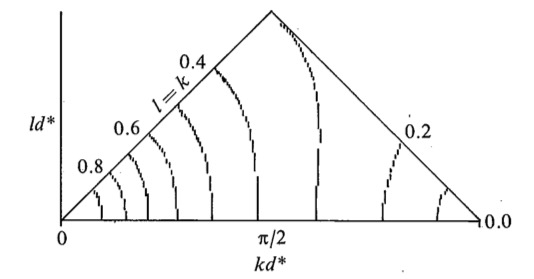
\includegraphics[keepaspectratio]{./pictest/pic461.jpg}}
\caption{}
\end{figure}

The wave number region in the figure is the same as in the earlier
diagrams, Figs. 2.3 and 4.1. Comparing the isolines of the present
figure with those of Fig. 2.3, where the effect of space differenc­ing
alone was considered, shows that the effect of time differencing on
phase speed is now not negligible. Implicit time differencing is seen to
result in a considerable retarda­tion of gravity waves of the same order
of magnitude as that due to centered space differencing.

To apply an implicit method it is necessary to solve the difference
system for variables at level n + 1.

With an ordinary oscillation equation, \texttt{h2.7} in
\texttt{Chapter2}, this can be done very simply. For the system
\texttt{b6.1} it is more complex. The quantities \(\delta_{x}u^{n + 1}\)
and \(\delta_{y}v^{n + 1}\) can be eliminated from the third equation by
applying operators \(\delta_{x}\) and \(\delta_{y}\) to the first and
second of these equa­tions and substituting the results into the third
equation. This gives an equation for the height which can be solved
using a number of standard methods : the most popular of these is the
\emph{relaxation method} which is discussed later in this section.

Two methods are used to deal with the advection, Coriolis, and other
terms of the governing equations, in atmospheric models. One of these,
the \emph{splitting method}, will be discussed in the next section. The
other is the semi-implicit method. There is no advantage in using an
implicit method for these additional terms of the governing equations.
They are associated with slower phase speeds, and should not require
excessively small time steps for linear stability when calculated
explicitly. Thus, they can be calculated by an explicit scheme. Since
the trapezoidal implicit scheme is a two level scheme like the
forward-backward scheme, it is convenient to use the Adams-Bashforth
scheme for this purpose. Robert (1969) in a spectral model, and
subsequently Kwizak and Robert (1971) in a grid point model, chose,
however, to use the leapfrog scheme. We then need variables at the
middle of the time step used for the implicit differencing, and,
therefore, it has to be performed over a time interval of \(2\Delta t\).
However, the scheme is now less economical for gravity waves since these
steps have to be made separately for each of the two time levels stored
in the leapfrog scheme. In return, we have a differencing for the
advection and other additional terms that is neutral and more accurate
than Adams-Bashforth\textquotesingle s. Kwizak and Robert call this
combined scheme the \emph{semi-implicit} scheme. It has been used for a
number of years in the Canadian operational model, and is becoming
increasingly popular in some other operational numerical prediction
centres.

The usual procedure used for solving the semi-implicit difference system
for variables at time level \(n + 1\) will be illustrated for the
shallow water equations. These equations can be written in a compact
form

{\[\frac{\partial u}{\partial t} = - g\frac{\partial h}{\partial x} + A_{u}\]\[\frac{\partial v}{\partial t} = - g\frac{\partial h}{\partial y} + A_{v}\]\[\frac{\partial h}{\partial t} = - H\nabla\textbf{v} + A_{h}\]}

where \(A_{u}\), \(A_{v}\) and \(A_{h}\) denote the terms that were
omitted in the system \texttt{b4.8} describing the propagation of pure
gravity waves.

When we use leapfrog differencing for these additional terms, and
implicit differencing over a time interval \(2\Delta t\) for the gravity
wave terms and centered space differencing, \texttt{b6.6} is replaced by

{\[u^{n + 1} = u^{n - 1} - g\Delta t\left( \delta_{x}h^{n - 1} + \delta_{x}h^{n + 1} \right) + 2\Delta t A_{u}^{n},\]\[v^{n + 1} = v^{n - 1} - g\Delta t\left( \delta_{y}h^{n - 1} + \delta_{y}h^{n + 1} \right) + 2\Delta t A_{v}^{n},\]\[h^{n + 1} = h^{n - 1} - H\Delta t\left[ \left( \delta_{x}u + \delta_{y}v \right)^{n - 1} + \left( \delta_{x}u + \delta_{y}v \right)^{n + 1} \right] +  2\Delta t A_{h}^{n}\]}

We now apply the operator \(\delta_{x}\) to the first, and
\(\delta_{y}\) to the second of these equations, respectively, and add
the results. We introduce the notation

\[\delta_{xx}h = \delta_x(\delta_x h ) \qquad  \delta_{yy}h = \delta_y(\delta_y h )\]

We obtain

\[\left( \delta_{x}u + \delta_{y}v \right)^{n + 1} =
\left( \delta_{x}u + \delta_{y}v \right)^{n - 1} 
- g\Delta t \left[ ( \delta_{xx} + \delta_{yy} )h^{n - 1} 
+ ( \delta_{xx} + \delta_{yy} )h^{n + 1}\right] +
2\Delta t( \delta_{x}A_{u} + {\delta_{y}A}_{v})^{n}\]

Substituting the right-hand side into the third of \texttt{b6.7}, and
defining the "finite difference Laplacian" by

\[\mathbf{\nabla_d}^2 \equiv ( \delta_{xx} + \delta_{yy} )h,\]

we find

\[\text{  h}^{n + 1} = h^{n - 1} - 2H\Delta t\left( \delta_{x}u + \delta_{y}v \right)^{n + 1}
 + gH\left( \Delta t \right)^{2}\left( \mathbf{\nabla_d}{2}h^{n - 1} + \mathbf{\nabla_d}^{2}h^{n + 1} \right) 
 + 2\Delta t\left\lbrack A_{h} - H\Delta t\left( {\delta_{x}A}_{u} + {\delta_{y}A}_{v} \right) \right\rbrack\]

Using, in addition, the definitions

\[F^{n + 1} \equiv h^{n + 1} - 2H\Delta t \left( \delta_{x}u + \delta_{y}v \right)^{n + 1} + gH(\Delta t)^{2}\mathbf{\nabla_d}^2 h^{n + 1},\]\[G^{n} \equiv 2\Delta t \left\lbrack A_{h} - H\Delta t\left( {\delta_{x}A}_{u} + {\delta_{y}A}_{v} \right) \right\rbrack^{n}\]

this can be written as

{\[h^{n + 1} - gH(\Delta t )^{2}\mathbf{\nabla_d}^{2}h^{n + 1} = F^{n + 1} + G^{n}\]}

The terms have been arranged to show that at time level n the right-hand
side is known at all space grid points. Once this equation has been
solved for the values \(h^{n + 1}\), \(u^{n + 1}\) and \(v^{n + 1}\) can
be obtained directly from the first and second of \texttt{b6.7}. We now
consider ways of solving \texttt{b6.8}.

The quantity \(\mathbf{\nabla_d}^{2}h\) on the left side of
\texttt{b6.8} is an approxi­mation to \(\nabla^{2}h\). Using the
notation of \texttt{figg:462}, it can be written as

\begin{figure}
\centering
\pandocbounded{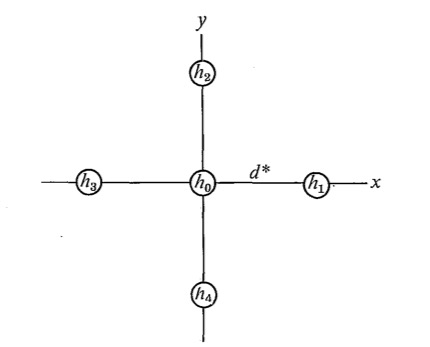
\includegraphics[keepaspectratio]{./pictest/pic462.jpg}}
\caption{}
\end{figure}

{\[\mathbf{\nabla_d}^2 h = \frac{1}{4(d^*)^2}\left( h_{1} + h_{2} + h_{3} + h_{4} - 4h_{0} \right)\]}

Thus, \texttt{b6.8} is a finite difference approximation to an elliptic
equation

\[\nabla^{2}h + ah + b\left( x,y \right) = 0\]

To solve such an equation, it is necessary to know the values of
\(h(x,y)\) at the boundaries of the computation region. For a numerical
solution we write \texttt{b6.8} at each of the interior grid points
where the variable h is carried. In this way we obtain a system with one
equation for each interior grid point. There is one unknown for each
grid point. In each of the equations, except the equations for points
adjacent to the boundary, there are five of these unknowns. There are no
difficulties in principle in solving such a system of linear equations,
but, since the number of equations is normally exceedingly large, of the
order of 1000 or more, it is not obvious how to set about it.

The method usually used is the relaxation method. This consists of the
following steps.

a) An arbitrary guess is made for the field \(h^{n + 1}\). Usually the
field of the preceding time step, \(h^{n}\), is taken as this first
guess.

b) At each of the grid points the value \(h^{n + 1}\) is changed so as
to satisfy the difference equation, in our case \texttt{b6.8}. These
changes can be made simultaneously at all grid points (simultaneous or
Richardson relaxation), or sequen­tially, point by point (sequential
oxLiebmann relaxation).

c) The preceding step is repeated as many times as needed to make the
change at every point less than some preassigned small value.

The relaxation method always converges. Experience shows that the
convergence is faster for sequential relaxa­tion, and also if the
changes calculated to satisfy the equation exactly are multiplied by a
factor having a value between 1 and 2 (overrelaxation factor) before
being added on. For a particular problem the optimum value of this
overrelaxation factor can easily be found by numerical experiments, in
which the number of iterations required is plotted as a function of the
value of the overrelaxation factor. This optimum value can be shown to
be not much less than 2. More details on the relaxation method can be
found in textbooks by Thompson (1961) and by Haltiner (1971).

The algebraic system given by equations of the type \texttt{b6.8} can
also be solved by \emph{direct methods} (e.g. Kreiss and Oliger, 1973,
p. 54). Direct method can be more efficient than the relaxation
procedure ; thus, they are typically used when relaxation requires very
large compu­tation time, as may happen, for example, in convection
studies. When implicit schemes are used for simulation or prediction of
large scale atmospheric motions, the time needed for relaxation is
several times less than the time needed for other steps of the
integration procedure, so that only a small fraction of the total
computer time can be saved by using a faster direct method. For that
reason the use of direct methods, requiring a larger programming effort,
is not popular in these models.

Generalization to the three-dimensional case of the procedure for
solving the semi-implicit system for variables at level \(n + 1\)
outlined here is not quite trivial. The reader is referred to the paper
by Robert \emph{et al}. (1972).

Implicit schemes were first used extensively in atmo­spheric models by
Marchuk (Marchuk, 1967). With the semi-implicit scheme it is also
possible to construct an economical grid analogous to the Eliassen grid
for the leapfrog scheme ; the appropriate space-time stagger­ing of the
variables was pointed out by Gerrity and McPherson (1971). A
semi-implicit scheme somewhat different from the one outlined here has
been developed by Burridge, and is now used in the British operational
model (Burridge and Hayes, 1974). Implicit and semi-implicit schemes are
undoubtedly the most efficient schemes used in atmospheric models. To
achieve this economy we have to put additional effort into solving an
elliptic equation. Furthermore they are associated with an appreciable
deceleration of gravity waves. Thus, the implicit schemes do not seem
suitable for the study of details of the geostrophic adjustement
process. How­ever, this deceleration does not appear particularly
harmful for the simulation and prediction of the large-scale
quasi-geostrophic motions. For example, Kwizak and Robert (1971) have
found that barotropic 5-day forecasts made with explicit differencing
and time steps of 10 min are almost identical to those made with
semi-implicit differencing and time steps of 60 min. Later Robert et al.
(1972) have calculated the differences be­tween 5-day forecasts obtained
using 30 and 60 min time steps for a baroclinic 5-leveI semi-implicit
model. These differences were found to be insignificant compared to
other sources of error normally present in numerical models. However,
the model used for these experiments did not include topography, surface
friction, and other physical processes ; one might expect the
deceleration of gravity waves to have a more noticeable effect when
these physical processes (e.g. the release of latent heat) are present,
since then the gravity waves should be more significant. On the other
hand, the computation time saved by the implicit differencing can be
used to reduce the grid size on the computation. This would decrease the
phase speed error for all the waves, including the gravity waves.

\subsection{\texorpdfstring{\textbf{The splitting or Marchuk
method}}{The splitting or Marchuk method}}\label{the-splitting-or-marchuk-method}

The complexity of the system of hydrodynamic equa­tions, that is, the
simultaneous presence of a number of physical factors, may cause some
difficulties. One difficulty was mentioned in the preceding section : if
we wanted to approximate \texttt{b6.6} using a fully implicit scheme we
would obtain a system for the variables at level that is practically
impossible to solve. Also since different physical factors are present
in this system we will nor­mally wish to use different schemes for terms
associated with them. Thus, considering the linearized system with
advection and gravity wave terms,

{\[\frac{\partial u}{\partial t} + c\frac{\partial u}{\partial x} + g\frac{\partial h}{\partial x} &= 0\]\[\frac{\partial h}{\partial t} + c\frac{\partial h}{\partial x} + H\frac{\partial u}{\partial x} &= 0\]}

we might wish to use one scheme for the advection terms, and another for
the gravity wave terms — in much the same way as was done within the
semi-implicit scheme. In such a situation, even though both of the
schemes to be used are stable considered one at a time, we cannot be
certain that the scheme obtained as a combination of the two will also
be stable. An example where it is not was given by Kasahara (1965).

These problems can be avoided by using the \emph{splitting method}. The
idea of this method is to construct schemes for a complex system of
equations so that \emph{within each time step} this system is split into
a number of simpler subsystems, which are then solved consecutively one
at

a time. In the case of \texttt{b7.1}, within a given time step, we could
first solve the system of advection equations

{\[\frac{\partial u}{\partial t} + c\frac{\partial u}{\partial x} = 0\]\[\frac{\partial h}{\partial t} + c\frac{\partial h}{\partial x} = 0\]}

Denote the provisional values \(u^{n + 1}, h^{n + 1}\) obtained in this
way by \(u^{*},h^{*}\). Use these values at the beginning of the time
step for solving the remaining subsystem

{\[\frac{\partial u}{\partial t} + g\frac{\partial h}{\partial x} = 0\]\[\frac{\partial h}{\partial t} + H\frac{\partial u}{\partial x} = 0\]}

The values \(u^{n + 1}\), \(h^{n + 1}\), obtained after solving also
this other subsystem, are now taken as actual approximate values of
these variables at the level \(n + 1\). The procedure is repeated in
each following time step.

A solution obtained by the splitting method will repre­sent a consistent
approximation to the true solution. This can be proved easily for a
particular choice of schemes for solving the subsystems. The approximate
values of the dependent variables then have to approach the true values
as the time step approaches zero.

To study the stability of schemes constructed by the splitting method,
we consider the example above. Denote by \(\lambda_{a}\) and
\(\lambda_{b}\) the values of \(\lambda\) of the schemes chosen for the
numerical solution of subsystems \texttt{b7.2} and \texttt{b7.3},
respectively. Then, we have

\[u^{*} &= Re\left( \lambda_{a}\lambda^{n}\widehat{u}e^{ikx} \right)\]\[h^{*} &= Re\left( \lambda_{a}\lambda^{n}\widehat{\lambda}e^{ikx} \right)\]

and

\[u^{n + 1} = Re\left( \lambda_{b}\lambda_{a}\lambda^{n}\widehat{u}e^{\text{ikx}} \right)\]\[h^{n + 1} = Re\left( \lambda_{b}\lambda_{a}\lambda^{n}\widehat{u}e^{\text{ikx}} \right)\]

Therefore, we find,

\[\lambda = \lambda_{b}\lambda_{a}\]

and

\[\left| \lambda \right| = \left| \lambda_{b} \right|\left| \lambda_{a} \right|\]

Thus, if both of the schemes chosen for the solution of subsystems
\texttt{b7.2} and \texttt{b7.3} are stable, the combined scheme
constructed by the splitting method will also be stable. This conclusion
can be generalized for an arbi­trary system of equations and number of
subsystems.

When applying the splitting method, we do not neces­sarily have to use
equal time steps for each of the subsys-This may well be the main
advantage of the splitting method : we can choose a relatively long time
step for the subsystem governing a slow process, advection in the
present example, and then use a number of smaller steps to calculate the
faster process. Since the advection process is the most expensive in
computation time within the primitive equations, significant economies
can be accomplished in this way. A disadvantage of the method is that
calculation of the effects of different physical factors one at a time
usually leads to an increase in the truncation error. For example,
Burridge and Hayes (1974) suggest that the technique of splitting the
governing equations into advection and adjustment stages does not allow
time steps longer than 12 to 15 min if the time-truncation is not to
become significant.

The splitting method was first used in atmospheric models by Marchuk
(Marchuk, 1967); thus, in mete­orology it is also known as the
\emph{Marchuk method}. It would appear that the splitting method is used
for most atmospheric models in the Soviet Union. The splitting technique
is used also in the British operational model (Burridge and Hayes,
1974), and in a limited area model by Lepas and his collaborators (Lepas
et al., 1974).

\subsection{\texorpdfstring{\textbf{Two-grid-interval
noise}}{Two-grid-interval noise}}\label{Section4.8}

Unless we are using the lattice (C) shown in \texttt{figg:421} we will
always have a problem with two-grid-interval waves. These are false
stationary waves appearing as neutral solutions of the difference
equations for gravity waves. When the Coriolis terms are also present,
as seen in Section \texttt{Section4.3}, the two-grid-interval waves
appear with false low frequencies as pure inertia waves, or, with
lattice (D), as stationary waves.

A number of methods have been used to cope with this. In many models
dissipative schemes are used to give maximum damping for the
two-grid-interval wave, or lateral diffusion is added with relatively
large diffusion coefficients. The appearance of excessive
two-grid-interval noise is thereby suppressed. However, instead of
attacking the \emph{consequences} of inadequacies in a simula­tion of a
physical process, it is generally better to look for a method that would
achieve a physically correct simulation of that process, and thus
eliminate the cause of the difficulty, One method this kind for dealing
with the two-grid-interval wave problem has been suggested and used by
Arakawa (1972). It consists of an intermittent use of uncentered space
differencing within the gravity wave terms, performed alternately on
opposite sides of the central point.

Mesinger (1973) showed how two-grid-interval wave noise could be
prevented in some cases even by using cen­tered differencing; this
method will be outlined briefly here. We consider the system of
linearized gravity wave equations

{\[\frac{\partial u}{\partial t} + g\frac{\partial h}{\partial x} &= 0\]\[\frac{\partial v}{\partial t} + g\frac{\partial h}{\partial y} &= 0\]\[\frac{\partial h}{\partial t} + H\nabla\cdot\mathbf{v} &= 0\]}

Consider any two neighbouring height points for example within the
lattice (E). A height perturbation at one of these points cannot affect
the other point because there is no velocity point in between ; this
velocity is needed to cause a height change at the other point through
the divergence term in the continuity equation. To circum­vent this
difficulty we can introduce auxiliary velocity points midway between the
height points. Velocity components at these auxiliary points can be
assumed equal to an average of velocities at the two neighbouring
velocity points at the beginning of a time step, and the acceleration
contributions can then be evaluated and added to these initial values to
obtain components at the middle or at the end of the time step. Only the
velocity components and accelerations along directions joining the two
height points are needed, and these accelerations can be calcu­lated
using the height values at the two points. The resulting velocity
components can then be used for a more accurate calculation of the
divergence term in the conti­nuity equation. In this way schemes are
obtained in which a height perturbation at a single grid point is
propagated by gravity waves to all the other height grid points.
Therefore there can be no grid-splitting and two grid-interval noise in
the height field. Since a velocity perturbation can propagate as a
gravity wave only by exciting height perturbations, the procedure will
prevent false two-grid-interval noise in all the variables.

We shall illustrate this procedure using the implicit scheme,
\texttt{b6.1}. The velocity components at regular velocity points are
computed in the same way as before, so the first two equations of that
system remain unchanged. To calculate the velocity divergence in the
continuity equation we define auxiliary velocity points midway between
the neighbouring height points, as shown by the circled numbers 5, 6, 7
and 8 in \texttt{figg:481}. Using the system \(x^{'},y^{'}\) shown in
this figure, components \(u\) are needed at points 5 and 7, and
components v\textquotesingle{} at points 6 and 8.

At the beginning of the time step \(\Delta t\) these components are
obtained by

\begin{figure}
\centering
\pandocbounded{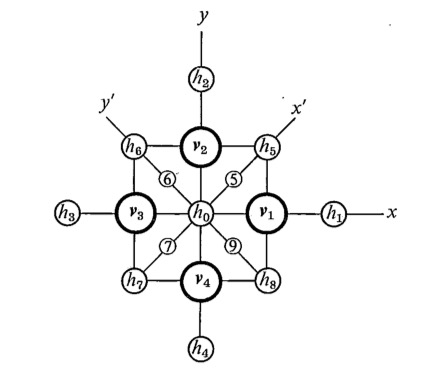
\includegraphics[keepaspectratio]{./pictest/pic481.jpg}}
\caption{}
\end{figure}

space-averaging, that is

\[u^{'n} &= \frac{\sqrt{2}}{2}\left( {\overline{u}}^{y'} + {\overline{v}}^{y'} \right)^{n},\]\[v^{'n} &= \frac{\sqrt{2}}{2}\left( - {\overline{u}}^{x'} + {\overline{v}}^{x'} \right)^{n}.\]

An overbar denotes a two-point average taken along the direction
indicated following the bar sign. Acceleration contributions are added
to these initial values to obtain values at the end of the time step,

\[u^{'n + 1} &= u^{'n} - g\Delta t\frac{1}{2}\left( \delta_{x'}h^{n} + \delta_{x'}h^{n + 1} \right)\]\[v^{'n + 1} &= v^{'n} - g\Delta t\frac{1}{2}\left( \delta_{y'}h^{n} + \delta_{y'}h^{n + 1} \right)\]

The velocity divergence in the continuity equation can now be
approximated by

\[\frac{1}{2}\left( \delta_{x}u + \delta_{y}v \right) + \frac{1}{2}\left( \delta_{x}u^{'} + \delta_{y}v^{'} \right)\]

giving equal weight to all eight directions of the lattice. In this way
the implicit approximation to the continuity equation may be obtained as

{\[h^{n + 1} = h^{n} - H\Delta t\left( \delta_{x}u + \delta_{y}v \right)^{n} 
+ \frac{1}{4}gH( \Delta t)^{2}\left( \nabla_{0}^{2}h^{n} + \nabla_{0}^{2}h^{n + 1} \right)\]}

Here the velocity components at level \emph{n + 1} have already been
eliminated using the first two of \texttt{b6.1}, and

{\[\nabla_{0}^{2} \equiv \frac{1}{4d^{2}} \times \left[ h_{1} + h_{2} + h_{3} + h_{4} + 2\left( h_{5} + h_{6} + h_{7} + h_{8} \right) - 12h_{0} \right]\]}

This is again a finite difference approximation to \(\nabla^{2}h\), but
now it is calculated using the height values of nine neigh­bouring
height points.

Comparing this scheme with the standard implicit scheme of Section
\texttt{Section4.6}, the only modification is that this nine-point
Laplacian has replaced the five-point Laplacian \texttt{b6.9} in the
continuity equation. This allows propagation of gravity waves between
all height points of the grid, thus admitting no false space noise in
the height field. A more detailed analysis of the properties of the
scheme can be found in Mesinger (1973). The modification, for example,
has no effect on the uncondi­tional stability of the implicit scheme ;
however, instead of being neutral for all waves, the scheme now damps
shorter waves to some extent. The modified scheme has a smaller
truncation error than the unmodified scheme.

Analogous modifications of some other schemes have been discussed in
papers by Janjic (1974) and Mesinger (1974). All of these papers show
that the modified schemes are strikingly superior in the case of a
stationary circular vortex, forced at a single height grid point. A note
by Mesinger and Janjic (1974) provides, further­more, a dramatic
illustration of the advantages of the proposed method in the case of a
limited area model, requiring lateral boundary conditions to be
prescribed. In a 5-level model using the unmodified forward-back­ward
scheme, intense short-wave noise was generated at the boundaries of the
region, a problem noticed also by earlier investigators (e.g. Miller
\emph{et al}., 1972 ; Krishnamurti et al., 1973). With the scheme
modified along these lines, however, there were no difficulties due to
the prescribed boundary conditions, even with no lateral diffusion in
the model.

It is important to be aware that this method is not attempting to
improve the calculation of short gravity waves of wave lengths close to
two grid intervals. At this scale the finite difference representation
is very poor, and significant improvements in accuracy can hardly be
expected. The problem is that gravity waves, with longer wave lengths
can propagate independently on individual (C) type subgrids, and thus
erroneously appear to have wave lengths close to two grid intervals.
Thus, we are confronted with a kind of aliasing error. The proposed
method enables these waves to appear with wave lengths close to their
physical value instead in the noise region with wave lengths close to
two grid intervals.

\subsection{\texorpdfstring{\textbf{Time noise and time
filtering}}{Time noise and time filtering}}\label{time-noise-and-time-filtering}

In addition to the appearance of spurious short-wave noise in space,
spurious short-wave noise in time, that is, high frequency noise can
appear in numerical models.

One mechanism causing this when the leapfrog scheme is used for
nonlinear equations is the separation of solutions at alternate time
steps, generating two-grid-interval noise in time. Such separation is
illustrated in a paper by Lilly (1965, p. 23).

High frequency noise appears in atmospheric models also as a result of
difficulties in observing initial condi­tions representative of the
large scale atmospheric motions. The observed initial conditions contain
instru­mental errors, are influenced by meso and small scale motions,
are not known at grid points of the model, and, finally, are completely
absent over relatively large areas of the globe. As a result of all of
these factors, if initial grid point values are interpolated directly
from the observed data the numerical forecasts will contain spurious
gravity waves of unrealistically large amplitudes.

In the early successful integrations of the primitive equations these
problems were partially by-passed by obtaining the initial winds from
the initial geopotential fields as a solution of the \emph{balance
equation} — the equation obtained by assuming the initial velocity
divergence and its time derivative to be equal to zero. Initial
conditions prepared in this way (e.g. Haltiner, 1971) prevent exces­sive
high-frequency gravity wave noise.

It is now generally accepted that this is not the best way of preparing
the initial conditions. First, the wind data are not used when solving
the balance equation, and some information is lost. It has also been
shown (e.g. Phillips, 1960b ;Winninghoff, 1968) that the presence of a
realistic initial divergent wind field should have a beneficial effect
on the forecast, Finally, an increasing fraction of the observations are
now continuous, and in time not obtained at specific times. The methods
being used to extract the maximum information from this type of data
rely more on running a prediction model to adjust the data in space and
time (e.g. Bengtsson, 1975). In such an integration relatively intense
high frequency noise is generated.

The first of the mechanisms mentioned here, separation of solutions at
alternate time steps, has to be suppressed in some way — otherwise it
may lead to a complete breakdown of the integration. One method that is
used for this purpose is an intermittent step made with a two level
scheme. A weakness of such a procedure is that the choice of the
solution that is eliminated is arbi­trary.

Experience shows that the noise generated by assi­milation of the
observed data typically dies out to an acceptable level in about 24
hours of simulated time due to geostrophic adjustment. However, it may
be desirable to accelerate this adjustment by appropriate numerical
techniques. The Matsuno scheme can be used for this purpose.

Another method that can be used to increase the damping of high
frequency noise in atmospheric models is \emph{time filtering}
originally proposed by Roberts (1966). To apply this at least three
consecutive values of the function to be filtered are needed. We shall
consider the simplest case where this minimum number of three values is
used. It suffices to consider one function only, which we assume to be a
solution of the oscillation equation. Thus, we consider the function

{\[U\left( t \right) = U\left( 0 \right)e^{i\omega t}\]}

where the values \(U\left( t - \Delta t \right)\), \(U\left( t \right)\)
and \(U\left( t + \Delta t \right)\), are known.

We shall first examine the effect of changing only the middle of these
three values using the relation

{\[\overline{U(t)} = U(t) + \frac{1}{2}S  \left[ U\left( t - \Delta t \right) - 2U\left( t \right) + U\left( t + \Delta t \right) \right]\]}

known as the \emph{centered filter}. The overbar now denotes the
filtered value of a function, and \(S\) is the \emph{filter parameter}.
The expression within the square bracket in \texttt{b9.2} is
pro­portional to the simplest approximation to the second derivative in
time ; thus, for sufficiently small positive values of \(S\) application
of the filter \texttt{b9.2} will decrease the curvature in a graph of
the three values of \(U(t)\)

For a quantitative analysis of the effect of the filter we define

{\[\overline{U(t)} \equiv R U(t)\]}

where the complex factor \(R\) is called the \emph{response} of the
filter. When this is substituted into \texttt{b9.2} and we use
\texttt{b9.1}, we obtain

{\[R = 1 - S\left( 1 - \cos{\omega\Delta t} \right)\]}

It is convenient to define \(R \equiv \left| R \right|e^{i\delta}\).

We can then say that the phase change \(\delta\) resulting from the
centered filter is zero, and that within the CFL stability criterion and
for small positive values of \(S\) the amplitude factor
\(\left| R \right|\) exerts a damping effect increasing with increasing
frequencies.

When, however, a filter is continually applied during a numerical
integration, the value \(U\left( t - \Delta t \right)\) has already been
changed prior to changing \(U(t)\). It is then appro­priate to consider
the filter

{\[\overline{U(t)} = U\left( t \right) + \frac{1}{2}S \left\lbrack \overline{U}\left( t - \Delta t \right) - 2U\left( t \right) + U\left( t + \Delta t \right) \right\rbrack\]}

Asselin (1972) calls this the basic time filter. A procedure like the
one used in deriving \texttt{b9.4} now gives

{\[R = \frac{( 2 - S )^{2} + 2S^{2}\left( 1 - \cos{\omega\Delta t} \right)}{( 2 - S^{2} ) + 4S\left( 1 - \cos{\omega\Delta t} \right)}e^{i\omega\Delta t}.\text{        }\]}

Thus, there is now a phase change that is different from zero; however,
it is small for small values of \(\omega\Delta t\). The amplitude factor
is not much different from that of the centered filter for small values
of \(S\). More details can be found in the paper by Asselin.

An analysis of the effect of the time filter for some particular choices
of time differencing schemes — the leapfrog, implicit and semi-implicit
schemes — can also be found in the paper by Asselin. We find, for
example, that the time filter in conjunction with the leapfrog scheme
can give a procedure damping the high frequencies in a more selective
way than the Matsuno scheme — less for low frequencies and more for high
frequencies. Since the computer time needed for application of the
filter is relatively small, this means that one obtains a better result
with only about half of the computer time. However, the application of
the filter does require the storage of the time dependent variables at
three time levels, that is, at one level more than with the standard
leapfrog scheme.

Using an analogous approach one can analyze the effect of smoothing and
filtering in space. The reader is referred to a review article by
Shapiro (1970) or the textbook by Haltiner (1971). It is, however, not
obvious that there are physical or computational reasons for using
two-dimensional space filtering in atmospheric models.

\subsection{\texorpdfstring{\textbf{Dissipation in numerical
schemes}}{Dissipation in numerical schemes}}\label{dissipation-in-numerical-schemes}

In concluding this chapter we add, following Arakawa (1970), a few
remarks regarding the role of dissipation that may be inherent in
numerical schemes. The discus­sion of the preceding chapter shows that
the use of dissipative schemes for the advection process should be
avoided — provided care is taken to avoid a false cascade of energy to
short waves. However, such short waves can still be generated as a
result of false reflections at boundaries on the down-stream side of the
region (Mat­suno, 1966c), or false reflections at sudden jumps in the
grid size, or at places where coefficients change rapidly. The use of
dissipative advection schemes at those places, and only at those places,
is justified.

The situation is different when we are now considering the
gravity-inertia wave terms, governing the geostrophic adjustment
process. This process is a result of the dis­persion of high frequency
waves. Use of a frequency-selective dissipative scheme will make these
high fre­quency waves damp out at a faster rate, and thus acce­lerate
the adjustment process, although the actual phy­sical process is
dispersive rather than dissipative. This gives an effect much the same
as that of time filtering. Therefore, if we are only interested in the
final result of the geostrophic adjustment process, dissipation in the
gravity-inertia wave terms may be helpful, especially when the high
frequency waves are predominantly unphysical. If we are interested in
the high frequency waves themselves, the use of a dissipative scheme
must, of course, be avoided.

REFERENCES

Марчук, Г. И., 1967. Численные методы в прогнозе
погоды. Ленинград. Гидрометеорологическое
издательство, 356 стр.

Ames, W. F., 1969. Numerical Methods for Partial Differential Equations.
London, Nelson. 291 pp.

Anderson, D. and Fattahi, В., 1974. A comparison of numerical solutions
of the advective equation. J. Atmos. Sci., 31, 1500-1506.

Arakawa, A., 1966. Computational design for long-term numerical
integration of the equations of fluid motion : Two dimensional
incompressible flow. Part I. J. Comput. Phys., 1, 119-143.

— 1970. Numerical simulation of large-scale atmospheric
motions.Numerical Solution of Field Problems in Continuum Physics, Proc.
Symp. Appl. Math., Durham, N. C, 1968. SIAM-AMS Proc, 2, 24-40.

— 1972. Design of the UCLA general circulation model. Numerical
Simulation of Weather and Climate, Dept. of Meteorology, Univ. of
California, Los Angeles, Tech. Rept. 7, 116 pp.

—- and Lamb, V. R., 1976. Computational design of the UCLA General
Circulation Model. To be published in Methods in Computational Physics,
Academic Press, New York.

Asselin, R., 1972.Frequency filter for time integrations. Mon. Wea.
Rev., 100, 487-490.

Bengtsson, L., 1975. 4-dimensional assimilation of meteorological
observations.WMO/ICSU Joint Organizing Committee, GARP Publications
Series No. 15, 76 pp.

Bjerknes, V., 1904. Das Problem der Wettervorhersage,
betrachtetvomStandpunkte der Mechanik und der Phvsik. Meteor.
Zeit-schr., 21, 1-7.

Burridge, D. M. and Hayes, F. R., 1974. Development of the British
operational model. The GARP Programme on Numerical Experimentation,
Rept. 4, 102-104.

Charney, J. G., 1966. Some remaining problems in numerical weather
prediction.Advances in Numerical Weather Predic­tion, Hartford, Conn.,
Travelers Research Center, Inc., 61-70.

—, Fjortoft, R. and von Neumann, J., 1950. Numerical integration of the
barotropicvorticity equation.Tellus, 2, 237-254.

Courant, R., Friedrichs, K. and Lewy, H., 1928.
UberdiepartiellenDifferenzengleichungen der mathematischenPhysik. Math.
Annalen, 100, 32-74.

— and Hilbert, D., 1953. Methods of Mathematical Physics, Vol. I. New
York, Interscience. 562 pp.

Cullen, M. J. P., 1974. Integration of the primitive equations on a
sphere using the finite element method. Quart. J. Roy. Meteor. Soc, 100,
555-562.

Deardorff, J. W., 1974. Three-dimensional numerical study of the height
and mean structure of a heated planetary boundary layer. Boundary-Layer
Meteor.,7, 81-106.

Egger, J., 1971. Mindestgrösse von Gebirgen und Konvektions-gebieten,
die in den Modellen der numerischen Vorhersage berück­sichtigt werden
können. Beitr. Phys. Atmos., 44, 245-271.

Eliassen, A., 1956. A procedure for numerical integration of the
primitive equations of the two-parameter model of the atmosphere.
Large-Scale Synoptic Processes, Dept. of Meteorology, Univ. of
California, Los Angeles, Sci. Rept. 4, 53 pp.

Fischer, G., 1959. Ein numerisches Verfahren zur Errechnung von Windstau
und Gezeiten in Randmeeren. Tellus, 11, 60-76.

Fjortoft, R., 1953. On the changes in the spectral distribution of
kinetic energy for two-dimensional, nondivergentflow.Tellus5 225-230.

Gadd, A. J., 1974a.An economical explicit integration scheme.
Meteorological Office Tech. Note 44, 7 pp.

— 1974b. Fourth order advection schemes for the 10 level model.
Meteorological Office Tech. Note 45, 8 pp.

Gerrity, J. P., Jr. and McPherson, R. D., 1971. On an efficient scheme
for the numerical integration of a primitive-equation barotropic model,
i. Appl. Meteor.,10, 353-363.

Haltiner, G. J., 1971. Numerical Weather Prediction.New York Wiley, 317
pp.

Harlow, F. H. and Amsden, A.A., 1971. Fluid dynamics. Los Alamos
Scientific Laboratory of the Univ. of California, Mono­graph LA-4700,
115 pp.

Hinkelmann, K., 1959. Ein numerisches Experiment mit den primi­tiven
Gleichungen. The Atmosphere and the Sea in Motion, Rossby Memorial
Volume, New York, Rockefeiler Institute Press, 486-500.

Janjic, Z. I., 1974. A stable centered difference scheme free of
two-grid interval noise. Mon. Wea. Rev., 102, 319-323.

Jespersen, D. C, 1974.Arakawa\textquotesingle s method is a
finite-element method. J. Comput. Phys., 16, 383-390.

Kasahara, A., 1965.On certain finite-difference methods for fluid
dynamics. Mon. Wea. Rev., 93, 27-31.

— 1969. Simulation of the earth\textquotesingle s atmosphere. National
Center for Atmospheric Research, Boulder, Colo., NCAR Manuscript 69-27,
42 pp.

FCreiss, H. and Öliger J., 1973.Methods for the approximate solution of
time dependent problems.WMO/ICSU Joint Organizing Committee, GARP
Publications Series No. 10, 107 pp.

Krishnamurti, T. N., Kanamitsu, M., Ceselski, B. and Mathur, M. B.,
1973.Florida State University\textquotesingle s Tropical Prediction
Model.Tellus, 25, 523-535.

Kurihara, Y., 1965. On the use of implicit and iterative methods for the
time integration of the wave equation. Mon. Wea. Rev., 93, 33\^{}t6.

90

THE GRAVITY AND GRAVITY-INERTIA WAVE EQUATIONS

Kwizak, M. and Robert, A. J., 1971. A semi-implicit scheme for grid
point atmospheric models of the primitive equations. Mon. Wea. Rev., 99,
32-36.

Lax, P. D. and Wendroff, B., 1960. Systems of conservation laws.Commun.
Pure Appl. Math., 13, 217-237.

Leith, C., 1965.Lagrangian advection in an atmospheric model.WMO-IUGG
Symposium on Research and Development Aspects of Long Range Forecasting,
Boulder, Colo., 1964. WMO Tech. Note 66, 168-176.

Lepas, J., Benlareche, M., Coiffier, J., Finke, L. and Tagnit-Hammou,
A., 1974.Primitive equations model — implicit method for numerical
integration. The GARP Programme on Numerical Experimentation, Rept. 4,
65.

Lilly, D. K., 1965.On the computational stability of numerical solutions
of time-dependent non-linear geophysical fluid dynamics problems. Mon.
Wea. Rev., 93, 11-26.

Matsuno, T., 1966a. Numerical integrations of the primitive equa­tions
by a simulated backward difference method. J. Meteor. Soc. Japan, Ser.
2, 44, 76-84.

— 1966b. A finite difference scheme for time integrations of
oscilla­tory equations with second order accuracy and sharp cut-off for
high frequencies. J. Meteor. Soc. Japan, Ser. 2, 44, 85-88.

— 1966c. False reflection of waves at the boundary due to the use of
finite differences. J. Meteor. Soc. Japan, Ser. 2, 44, 145-157.

Mesinger, F., 1971. Numerical integration of the primitive equations
with a floating set of computation points : Experiments with a
barotropic global model. Mon. Wea. Rev., 99, 15-29.

— 1973. A method for construction of second-order accuracy differ­ence
schemes permitting no false two-grid-interval wave in the height
field.Tellus, 25, 444-458.

— 1974. An economical explicit scheme which inherently prevents the
false two-grid-interval wave in the forecast fields. Difference and
Spectral Methods for Atmosphere and Ocean Dynamics Problems, Proc.
Symp., Novosibirsk, 1973, Part II, 18-34.

— andJanjic Z. I., 1974. Noise due to time-dependent boundary conditions
in limited area models. The GARP Programme on Numerical Experimentation,
Rept. 4, 31-32.

Miller, B.I., Chase, P.P. and Jarvinen, B. R., 1972. Numerical
prediction of tropical weather systems. Mon. Wea. Rev., 100, 825-835.

Orszag, S. A., 1971. On the elimination of aliasing in finite-difference
schemes by filtering high-wavenumber components. J. Atmos. Sci., 28,
1074.

Phillips, N. A., 1956. The general circulation of the atmosphere : a
numerical experiment. Quart. J. Roy. Meteor. Soc, 82, 123-164.

— 1959. An example of non-linear computational instability. The
Atmosphere and the Sea in Motion, Rossby Memorial Volume, New York,
Rockefeller Institute Press, 501-504.

— 1960a. Numerical weather prediction.Advances in Computers, New York,
Academic Press, 1, 43-90.

— 1960b. On the problem of initial data for the primitive
equations.Tellus, 12, 121-126.

Platzman, G. W., 1958 .The lattice structure of the finite-difference
primitive and vorticity equations. Mon. Wea. Rev., 86, 285-292.

— 1963. The dynamical prediction of wind tides on Lake Erie. Meteor.
Monogr., 4, No. 26, 44 pp.

— 1964. An exact integral of complete spectral equations for un­steady
one-dimensional flow. Dynamical Prediction Group, Dept. of the
Geophysical Sciences, Univ. of Chicago, Tech. Rept. 16, 28 pp.

Richardson, L. F., 1922. Weather Prediction by Numerical Process.
London, Cambridge University Press/reprinted: Dover, 1965/. 236 pp.

Richtmyer, R. D., 1963. A survey of difference methods for non-steady
fluid dynamics. National Center for Atmospheric Research, Boulder,
Colo., NCAR Tech. Notes 63-2, 25 pp.

— and Morton, K. W., 1967. Difference Methods for Initial Value
Problems. New York, Interscience. 406 pp.

Robert, A. J., 1966. The integration of a low order spectral form of the
primitive meteorological equations. J. Meteor. Soc. Japan, Ser. 2, 44,
237-245.

— 1969. The integration of a spectral model of the atmosphere by the
implicit method.Proc. WMO/IUGG Symposium on Numerical Weather Prediction
in Tokyo, 1968. Meteor. Soc. Japan. VII-19-VII-24.

—, Henderson, J. and Turnbull, C, 1972. An implicit time integra­tion
scheme for baroclinic models of the atmosphere. Mon. Wea. Rev., 100,
329-335.

— 1974. Computational resolution requirements for accurate medium-range
numerical predictions. Difference and Spectral Methods for Atmosphere
and Ocean Dynamics Problems, Proc. Symp., Novosibirsk, 1973, Part I,
82-102.

Sawyer, J. S., 1972.Numerical weather prediction within World Weather
Watch — past, present and future.Tenth Anniversary of the World Weather
Watch, Geneva, WMO Publ. No. 342, 33-44.

Shapiro, R., 1970.Smoothing, filtering, and boundary effects. Rev.
Geophys. Space Phys., 8, 359-387.

Shuman, F. G., 1974. Analysis and experiment in nonlinear computa­tional
stability. Difference and Spectral Methods for Atmosphere and Ocean
Dynamics Problems, Proc. Symp., Novosibirsk, Part I, 51-81.

—, Brown, J. A. and Campana, K., 1975. A new explicit differencing
system for primitive equations.In preparation.

Sielecki, A., 1968.An energy-conserving difference scheme for the storm
surge equations. Mon. Wea. Rev., 96, 150-156.

Thompson, P. D., 1961. Numerical Weather Analysis and Prediction. New
York, Macmillan. 170 pp.

Winninghoff, F. J., 1968. On the adjustment toward a geostrophic balance
in a simple primitive equation model with application to the problems of
initialization and objective analysis.Ph. D. thesis, Dept. of
Meteorology, Univ. of California, Los Angeles, 161 pp.

Wurtele, M. G., 1961. On the problem of truncation error.Tellus, 13,
379-391.

Young, J. A., 1968. Comparative properties of some time differencing
schemes for linear and non-linear oscillations. Mon. Wea. Rev., 96,
357-364.

GARP PUBLICATIONS SERIES

No. 1 An Introduction to GARP

No. 2 COSPAR Working Group VI Report to JOC — Systems Possibilities for
an Early GARP Experiment (out of print)

No. 3 The Planning of the First GARP Global Experiment (out of print)

No. 4 The Planning of GARP Tropical Experiments (out of print)

No. 5 Problems of Atmospheric Radiation in GARP

No. 6 Numerical Experimentation Related to GARP

No. 7 The GARP Programme on Numerical Experimentation

No. 8 Parameterization of Sub-Grid Scale Processes

No. 9 The Basic Data Set Project

No. 10 Methods for the Approximate Solution of Time-Dependent Problems

No. 11 The First GARP Global Experiment — Objectives and Plans

No. 12 The Complete Atmospheric Energetics Experiment (CAENEX)

No. 13 The Air Mass Transformation Experiment (AMTEX)

No. 14 Modelling for the First GARP Global Experiment

No. 15 Four-Dimensional Assimilation of Meteorological Observations

No. 16 The Physical Basis of Climate and Climate Modelling

No. 17 Numerical Methods Used in Atmospheric Models

No. 18 The Monsoon Experiment (MONEX)

GARP SPECIAL REPORTS

No. 1 Report of Planning Conference on GARP — Brussels, March 1970

No. 2 Report of Interim Planning Group on GARP Tropical Experiment in
the Atlantic — London, July 1970

No. 3 Report of the First Session of the Tropical Experiment Council —
Geneva, February 1971

No. 4 Report of the First Session of the Tropical Experiment Board —
Geneva, February 1971

No. 5 Report of the Second Session of the Tropical Experiment Board —
Geneva, December 1971

No. 6 Report of the Third Session of the Tropical Experiment Board —
Geneva, April 1972 (out of print)

No. 7 Report of the Second Session of the Tropical Experiment Council —
Geneva, September 1972

No. 8 Report of the Planning Conference on the First GARP Global
Experiment — Geneva, September 1972

No. 9 Report of the Fourth Session of the Tropical Experiment Board —
Geneva, March 1973 (out of print)

No. 10 Report on Special Observing Systems for the First GARP Global
Experiment — Geneva, February 1973

No. 11 Report of the Fifth Session of the Tropical Experiment Board —
Geneva, December 1973

No. 12 Report of the Sixth Session of the Tropical Experiment Board —
Geneva, April 1974

No. 13 Report of the Meeting on Drifting Buoys for the First GARP Global
Experiment—Geneva, March 1974

No. 14 Report of the First Session of WMO Executive Committee
Inter-Governmental Panel on the\textquotesingle First GARP

Global Experiment — Geneva, October 1974 No. 15 Report of the Seventh
Session of the Tropical Experiment Board — Geneva, February 1975 No. 16
Report of the Meeting of Experts for the Development of a Data
Management Plan for the FGGE —

Washington, April 1975

No. 17 Report of the Second Session of WMO Executive Committee
Inter-Governmental Panel on the First

GARP Global Experiment — Geneva, September 1975 (in preparation) No. 18
Report of the Inter-Governmental Planning Meeting for the First GARP
Global Experiment — Geneva

February 1976

No. 19 Report of the Extraordinary Session of WMO Executive Committee
Inter-Governmental Panel on the

First GARP Global Experiment — Geneva, February 1976 No. 20 Report of
the Eighth Session of the Tropical Experiment Board — Geneva, May 1976
No. 21 Report of the Planning Meeting for the Monsoon-77 Experiment —
Colombo, Sri Lanka, May 1976 No. 22 Report of the Third Session of WMO
Executive Committee Inter-Governmental Panel on the First GARP

Global Experiment — Geneva, July 1976

By arrangement between ICSU and WMO, these publications are on sale and
copies can be obtained from the Secretariat of the World Meteorological
Organization, Case postale No. 5, CH-1211 Geneva 20, Switzerland.
